% ===================================================================================== %
%                                        Header                                         %
% ===================================================================================== %
\documentclass[10pt,t,xcolor=table,compress]{UWMadBeamer}

\usepackage{graphicx}
\usepackage{transparent}
\usepackage{textcomp}
\usepackage{lmodern}
\usepackage{amsmath}
\usepackage{setspace}
\usepackage{booktabs}
\usepackage{multirow}
\usepackage{appendixnumberbeamer}



% =============================================================================================== %
%                                     Math Commands                                               %
% =============================================================================================== %


% ---------------------------------------------------------------------------- %
%                                Square Root Tail                              %
% ---------------------------------------------------------------------------- %
\DeclareRobustCommand{\NthRootInTeX}[2]{\root #1 \of {#2\:\!}}

\DeclareRobustCommand{\SquareRootCore}[2]{
    \setbox0=\hbox{\ensuremath{\NthRootInTeX{#1}{#2}}}
    \dimen0=\ht0
    \advance\dimen0-0.2\ht0
    \setbox2=\hbox{\vrule height\ht0 depth -\dimen0}
    {\box0\lower0.47pt\box2}
}

\DeclareRobustCommand{\Sqrt}[2][]{
    \mathchoice{\SquareRootCore{#1}{#2}}
               {\SquareRootCore{#1}{#2}}
               {\SquareRootCore{#1}{#2}}
               {\SquareRootCore{#1}{#2}}
}



% ---------------------------------------------------------------------------- %
%                              Derivative Commands                             %
% ---------------------------------------------------------------------------- %
\newcommand{\bigdiffn}[4]{\dfrac{#1{}^{#4}}{#1 #3{}^{#4}} \left[ #2 \right]}
\newcommand{\gendiffn}[4]{\dfrac{#1{}^{#4} #2}{#1 #3{}^{#4}}}

\newcommand{\diff}[3][d]{
    \ifthenelse{\equal{p}{#1}}{
        \gendiffn{\partial}{#2}{#3}{}
    }{
        \ifthenelse{\equal{b}{#1}}{
            \bigdiffn{d}{#2}{#3}{}
        }{
            \ifthenelse{\equal{bp}{#1}}{
                \bigdiffn{\partial}{#2}{#3}{}
            }{
                \gendiffn{d}{#2}{#3}{}
            }
        }
    }
}

\newcommand{\diffn}[4][d]{
    \ifthenelse{\equal{p}{#1}}{
        \gendiffn{\partial}{#2}{#3}{#4}
    }{
        \ifthenelse{\equal{b}{#1}}{
            \bigdiffn{#2}{#3}{#4}
        }{
            \ifthenelse{\equal{bp}{#1}}{
                \bigdiffn{\partial}{#2}{#3}{#4}
            }{
                \gendiffn{#1}{#2}{#3}{#4}
            }
        }
    }
}

\newcommand{\bigdiff}   [2] {\diff[b]{#1}{#2}}
\newcommand{\pdiff}     [2] {\diff[p]{#1}{#2}}
\newcommand{\bigpdiff}  [2] {\diff[bp]{#1}{#2}}
\let\frac\dfrac
\newcommand{\subs}      [2][]{\ensuremath{{}_{#1\text{\scriptsize #2}}}}
\newcommand{\sups}      [2][]{\ensuremath{{}^{#1\text{\scriptsize #2}}}}
\newcommand{\oneo}      [1]  {\ensuremath{\frac{1}{#1}}}




\newcommand{\Density}{\ensuremath{\rho}\xspace}
\newcommand{\Temperature}{\ensuremath{T}\xspace}
\newcommand{\Pressure}{\ensuremath{P}\xspace}
\newcommand{\IntEnergy}{\ensuremath{i}\xspace}
\newcommand{\Entropy}{\ensuremath{s}\xspace}
\newcommand{\Enthalpy}{\ensuremath{h}\xspace}
\newcommand{\ThCond}{\kappa}
\newcommand{\Viscosity}{\mu}
\newcommand{\DiffCoef}{\ensuremath{D}\xspace}

\newcommand{\isat}{\ensuremath{\IntEnergy\subs[\!]{sat}}\xspace}
\newcommand{\Psat}{\ensuremath{\Pressure\subs[\!\!]{sat}}\xspace}
\newcommand{\Tsat}{\ensuremath{\Temperature\subs[\!\!\:]{sat}}\xspace}
\newcommand{\SubL}{\subs[\!\!\:]{\rule{0pt}{8pt}$\textstyle\ell$}}
\newcommand{\SubG}{\subs[\!\!\:]{$\mathit{g}$}}

\newcommand{\rhol}{\ensuremath{\rho\SubL}\xspace}
\newcommand{\rhog}{\ensuremath{\rho\SubG}\xspace}
\newcommand{\il}{\ensuremath{i\SubL}\xspace}
\newcommand{\ig}{\ensuremath{i\SubG}\xspace}
\newcommand{\rhoul}{\ensuremath{\rhou\SubL}\xspace}
\newcommand{\rhoug}{\ensuremath{\rhou\SubG}\xspace}
\newcommand{\rhoil}{\ensuremath{\rhoi\SubL}\xspace}
\newcommand{\rhoig}{\ensuremath{\rhoi\SubG}\xspace}
\newcommand{\alphal}{\ensuremath{\alpha\SubL}\xspace}
\newcommand{\alphag}{\ensuremath{\alpha\SubG}\xspace}

\newcommand{\tauSat}{\ensuremath{\tau\subs[\!\!\:]{sat}}\xspace}
\newcommand{\deltaL}{\ensuremath{\delta\subs[\!\!\:]{\rule{0pt}{8pt}$\textstyle\ell$}}\xspace}
\newcommand{\deltaG}{\ensuremath{\delta\subs[\!\!\:]{$\mathit{g}$}}\xspace}

\newcommand{\rhoc}  {\ensuremath{\rho\subs{c}}\xspace}
\newcommand{\Tc}    {\ensuremath{T\subs{c}}\xspace}

\newcommand{\Skip}[1][0.45em]{\\[#1]}
\newcommand{\TCS}    {Thermodynamic Coexistence System\xspace}
\newcommand{\TCSRef} {\hyperref[Eqn:TCS]{\TCS}\xspace}
\newcommand{\MCS}    {Mechanical Coexistence System\xspace}
\newcommand{\MCSRef} {\hyperref[Eqn:MCS]{\MCS}\xspace}

\newcommand{\Afe}{\ensuremath{A\subs{\textsc{fe}}}}
\newcommand{\HFE}{Helmholtz free energy\xspace}
\newcommand{\EOS}{equation of state\xspace}

\newcommand{\Space}{\ensuremath{z}\xspace}
\newcommand{\Time}{\ensuremath{t}\xspace}
\newcommand{\Speeds}{\ensuremath{\mathbf{\lambda}}\xspace}

\DeclareMathOperator{\Ln}{Ln}
\DeclareMathOperator{\Abs}{Abs}
\DeclareMathOperator{\Inf}{Inf}
\DeclareMathOperator{\Exp}{Exp}
\DeclareMathOperator{\Rez}{R}

\let\originalleft\left
\let\originalright\right
\renewcommand{\left}{\mathopen{}\mathclose\bgroup\originalleft\;\!}
\def\left#1{\mathopen{}\mathclose\bgroup\originalleft#1\:\!}
\def\right#1{\aftergroup\egroup\:\!\originalright#1}


%\DefineNewLength{\RowSkip}{1.0em}
%\newcommand{\skp}[1][0.45em]{
%    \ifthenelse{\equal{#1}{}}{
%        \\[\RowSkip]
%    }{
%        \\[#1]
%    }
%}

\newcommand{\Del}[1][]{
    \partial_{#1}
}

\newcommand{\Vector}[1]{
    \underline{#1}
}

\newcommand{\Tensor}[1]{
    \underline{\underline{#1}}
}

\newcommand{\qConRaw}{\mathbf{q}}
\newcommand{\qCon}{\ensuremath{\qConRaw}\xspace}
\newcommand{\qPer}{\ensuremath{\widehat{\qConRaw}}\xspace}
\newcommand{\qSS} {\ensuremath{\qConRaw^0}\xspace}

\newcommand{\ConSys}{
    \Psi
}

\newcommand{\ConSysHEM}[1][HEM]{
    \ConSys_{\!\mbox{\tiny #1}}
}


\newcommand{\Flux}{
    \mathbf{F}
}
\newcommand{\Source}{
    \mathbf{S}
}

\newcommand{\Weight}{\beta}


\newcommand{\FluxFun}[2][]{
    \mathbf{F}_{#1}\left(#2\right)
}

\newcommand{\SourceFun}[2][]{
    \mathbf{S}_{#1}\left(#2\right)
}

\newcommand{\ResidualFun}[2][]{
    \mathbf{R}_{#1}\left(#2\right)
}

\newcommand{\Jacobian}[1][]{
    \mathbb{J}\subs{#1}
}

\newcommand{\JacobGen}[2]{
  \Jacobian[{\scriptscriptstyle #1}](#2)
}

\newcommand{\JacobF}{
    \Jacobian[F]
}


\newcommand{\JacobS}[1]{
    \JacobGen{S}{#1}
}

\newcommand{\FluxSS}{
    \mathbf{F}^{0}
}

\newcommand{\SourceSS}{
    \mathbf{S}^{0}
}

\newcommand{\JacobFSS}[1][\,\,\!]{
    \mathbf{J}_{\!{\scriptscriptstyle F}}^{0}{}#1
}

\newcommand{\JacobSSS}[1][\,\,\!]{
    \mathbf{J}_{\!{\scriptscriptstyle S}}^{0}#1
}

\newcommand{\BigO}[1]{
    \ensuremath{\mathcal{O}\!\left(#1\right)}
}


\newcommand{\Correl}[2]{
    f^{\mbox{\scriptsize cor}}_{#1}\left(#2\right)
}

\newcommand{\LpNorm}[2][2]{
    \ensuremath{\lvert\!\lvert#2\rvert\!\rvert_{#1}}
}

\newcommand{\Nudge}{
    \ensuremath{\!\!\;}
}

\newcommand{\hfg}{
    \ensuremath{h_{\mbox{\scriptsize fg}}}
}



%\NewEnviron{BoxedAlgorithm}[1][H]{
%    \begin{center}
%        \begin{minipage}{0.999\textwidth}
%            \centering
%            \fcolorbox{black}{white}{
%                \centering
%                \begin{minipage}[t]{0.85\textwidth}
%                    \begin{algorithm}[#1]
%                        \BODY
%                    \end{algorithm}
%                \end{minipage}
%            }
%        \end{minipage}
%    \end{center}
%}


\DeclareRobustCommand{\TH}  {thermal hydraulics\xspace}
\DeclareRobustCommand{\THc} {Thermal hydraulics\xspace}
\DeclareRobustCommand{\THcc}{Thermal Hydraulics\xspace}
\DeclareRobustCommand{\THs} {thermal hydraulic\xspace}

\DeclareRobustCommand{\CLaw}  {conservation law\xspace}
\DeclareRobustCommand{\CLaws} {conservation laws\xspace}


\newcommand{\rhou}{\ensuremath{\rho{u}}\xspace}
\newcommand{\rhoi}{\ensuremath{\rho{i}}\xspace}

\newcommand{\tr}{\ensuremath{{}\sups{\textsc{T}}}}
\newcommand{\mdotloss}[1][]{\ensuremath{\dot{m}'''\subs[\!\!\!\!\!#1]{loss}}\xspace}
\newcommand{\Keff}{\ensuremath{K\subs{eff}}}

\newcommand{\POfRhoRhoi}{\ensuremath{P\left(\rho,\frac{\rhoi}{\rho}\right)}}


\newcommand{\EqnSkip}[1][3em]{\ensuremath{\mbox{\rule{0.5em}{#1}}}\\}
\newcommand{\psiEOS}{\ensuremath{\psi}\subs{\textsc{eos}}}




%\DefineNewLength{\BarredLetterHeight}{0pt}
%\DefineNewLength{\BarredLetterWidth}{0pt}

%\newcommand{\eBB}{
%    \ensuremath{
%        \settoheight{\BarredLetterHeight}{e} % Height in current context
%        \settowidth{\BarredLetterWidth}{e}   % Width  in current context
%        e\mbox{\hspace{-0.57\BarredLetterWidth}\rule{0.035em}{0.96\BarredLetterHeight}} % bar
%    }
%}

%\newcommand{\TableSkip}{\rule[-1.4em]{0pt}{3.3em} \\[0pt]}
\definecolor{Gray}{gray}{0.93}


\newcommand{\LedineggCriterion}{$\tfrac{\partial\Delta{P}}{\partial(\rhou)}\bigr\rvert_{\text{int}} \le 
                                 \tfrac{\partial\Delta{P}}{\partial(\rhou)}\bigr\rvert_{\text{ext}}$}
                                
                                
\newcommand{\etal}{et al.\xspace}
\newcommand{\etc}{etc.\xspace}
\newcommand{\eg}{e.g.\xspace}
\newcommand{\ie}{i.e.\xspace}


\newcommand{\rhok}{ \ensuremath{\alpha\rho\subs{\phi}}\xspace}
\newcommand{\rhouk} {\ensuremath{\alpha\rhou\subs{\phi}}\xspace}
\newcommand{\rhoik} {\ensuremath{\alpha\rhoi\subs{\phi}}\xspace}
\newcommand{\alphak}{\ensuremath{\alpha\subs{\phi}\xspace}}
\newcommand{\uk}{\ensuremath{u\subs{\phi}}\xspace}
\newcommand{\ik}{\ensuremath{i\subs{\phi}}\xspace}
\newcommand{\CVvol}[1][k]{\ensuremath{\Omega_\text{#1}}\xspace}
\newcommand{\MCvol}[1][m]{\ensuremath{\Omega_\text{#1}}\xspace}
\newcommand{\CVsurf}[1][k]{\ensuremath{\Gamma_\text{#1}}\xspace}
\newcommand{\MCsurf}[1][m]{\ensuremath{\Gamma_\text{#1}}\xspace}








    \let\Oldalpha     \alpha     \renewcommand{\alpha}     {\ensuremath{\Oldalpha     }\xspace}
    \let\Oldbeta      \beta      \renewcommand{\beta}      {\ensuremath{\Oldbeta      }\xspace}
    \let\Oldgamma     \gamma     \renewcommand{\gamma}     {\ensuremath{\Oldgamma     }\xspace}
    \let\Olddelta     \delta     \renewcommand{\delta}     {\ensuremath{\Olddelta     }\xspace}
    \let\Oldepsilon   \epsilon   \renewcommand{\epsilon}   {\ensuremath{\Oldepsilon   }\xspace}
    \let\Oldvarepsilon\varepsilon\renewcommand{\varepsilon}{\ensuremath{\Oldvarepsilon}\xspace}
    \let\Oldzeta      \zeta      \renewcommand{\zeta}      {\ensuremath{\Oldzeta      }\xspace}
    \let\Oldeta       \eta       \renewcommand{\eta}       {\ensuremath{\Oldeta       }\xspace}
    \let\Oldtheta     \theta     \renewcommand{\theta}     {\ensuremath{\Oldtheta     }\xspace}
    \let\Oldvartheta  \vartheta  \renewcommand{\vartheta}  {\ensuremath{\Oldvartheta  }\xspace}
    \let\Oldkappa     \kappa     \renewcommand{\kappa}     {\ensuremath{\Oldkappa     }\xspace}
    \let\Oldlambda    \lambda    \renewcommand{\lambda}    {\ensuremath{\Oldlambda    }\xspace}
    \let\Oldmu        \mu        \renewcommand{\mu}        {\ensuremath{\Oldmu        }\xspace}
    \let\Oldnu        \nu        \renewcommand{\nu}        {\ensuremath{\Oldnu        }\xspace}
    \let\Oldxi        \xi        \renewcommand{\xi}        {\ensuremath{\Oldxi        }\xspace}
    \let\Oldpi        \pi        \renewcommand{\pi}        {\ensuremath{\Oldpi        }\xspace}
    \let\Oldvarpi     \varpi     \renewcommand{\varpi}     {\ensuremath{\Oldvarpi     }\xspace}
    \let\Oldrho       \rho       \renewcommand{\rho}       {\ensuremath{\Oldrho       }\xspace}
    \let\Oldvarrho    \varrho    \renewcommand{\varrho}    {\ensuremath{\Oldvarrho    }\xspace}
    \let\Oldsigma     \sigma     \renewcommand{\sigma}     {\ensuremath{\Oldsigma     }\xspace}
    \let\Oldvarsigma  \varsigma  \renewcommand{\varsigma}  {\ensuremath{\Oldvarsigma  }\xspace}
    \let\Oldtau       \tau       \renewcommand{\tau}       {\ensuremath{\Oldtau       }\xspace}
    \let\Oldupsilon   \upsilon   \renewcommand{\upsilon}   {\ensuremath{\Oldupsilon   }\xspace}
    \let\Oldphi       \phi       \renewcommand{\phi}       {\ensuremath{\Oldphi       }\xspace}
    \let\Oldvarphi    \varphi    \renewcommand{\varphi}    {\ensuremath{\Oldvarphi    }\xspace}
    \let\Oldchi       \chi       \renewcommand{\chi}       {\ensuremath{\Oldchi       }\xspace}
    \let\Oldpsi       \psi       \renewcommand{\psi}       {\ensuremath{\Oldpsi}\xspace}
    \let\Oldomega     \omega     \renewcommand{\omega}     {\ensuremath{\Oldomega     }\xspace}
    \let\OldGamma     \Gamma     \renewcommand{\Gamma}     {\ensuremath{\OldGamma     }\xspace}
    \let\OldLambda    \Lambda    \renewcommand{\Lambda}    {\ensuremath{\OldLambda    }\xspace}
    \let\OldSigma     \Sigma     \renewcommand{\Sigma}     {\ensuremath{\OldSigma     }\xspace}
    \let\OldPsi       \Psi       \renewcommand{\Psi}       {\ensuremath{\OldPsi       }\xspace}
    \let\OldDelta     \Delta     \renewcommand{\Delta}     {\ensuremath{\OldDelta     }\xspace}
    \let\OldXi        \Xi        \renewcommand{\Xi}        {\ensuremath{\OldXi        }\xspace}
    \let\OldUpsilon   \Upsilon   \renewcommand{\Upsilon}   {\ensuremath{\OldUpsilon   }\xspace}
    \let\OldOmega     \Omega     \renewcommand{\Omega}     {\ensuremath{\OldOmega     }\xspace}
    \let\OldTheta     \Theta     \renewcommand{\Theta}     {\ensuremath{\OldTheta     }\xspace}
    \let\OldPi        \Pi        \renewcommand{\Pi}        {\ensuremath{\OldPi        }\xspace}
    \let\OldPhi       \Phi       \renewcommand{\Phi}       {\ensuremath{\OldPhi       }\xspace}


\setlength{\parskip}{0.5em}


\newenvironment{Itemize}
    {\begin{itemize}\setlength{\itemsep}{0.8em}\setlength{\leftmargin}{0.0em}\setlength{\labelwidth}{0em}}
    {\end{itemize}}



%\title{On the Stability of Natural Circulation Loops with Phase Change}
\title{On the Behavior of Natural Circulation Loops with Phase Change}
\institute{University of Wisconsin--Madison}
\department{Engineering Physics Department}
\author{Troy C. Haskin}
\date{2016/09/20}


\graphicspath{{./Graphics/}}
\logo{\transparent{0.1}\includegraphics[scale=0.22]{UWMadison-Crest}}



\setbeamersize{text margin left = 0.03\paperwidth}
\setbeamersize{text margin right = 0.03\paperwidth}


% =========================================================================== %
%                              Document                                       %
% =========================================================================== %
\begin{document}
 

% ======================================================= %
%                         Titlepage                       %
% ======================================================= %
\begin{frame}
    \titlepage
\end{frame}


% ======================================================= %
%                         Outline                         %
% ======================================================= %
\begin{frame}{Outline}
    \tableofcontents
\end{frame}



% ======================================================= %
%                       Introduction                      %
% ======================================================= %
\chapter{Introduction}

Stability of two-phase natural circulation systems is not a novel subject in-and-of itself.
However, this work aims to perform the analysis on a closed-loop geometry with unique characteristics to be discussed.
Motivation for this effort will be given from examination of a physical system.
Then, a literature review will be given that overviews the field of stability analysis in general.
Finally, some concluding remarks will be given pertaining to the goals of this work.

\IncludeSection{Section2-ReactorCavityCoolingSystem}
\newpage
\IncludeSection{Section3-Literature}

\section{Research Purpose}\label{Section:Purpose}

The contribution of this work to the two-phase stability literature is a combination of topics in one analysis.
First, this work uses a non-ideal, continuous \Acro{EOS} for water.
Rather than approximating liquid water as a stiffened gas \cite{hayward_compressibility_1967-1} or using tabulated values, a complete implementation of the equation of state of water from the \Acro{IAPWS} is used.
All thermodynamic and kinematic properties used in the simulations are calculated from the mechanically balanced mass and energy of the system.
Second, this work uses an implementation of a modern, nonlinear solver that accurately and conservatively calculates all of the steady-states from which the linear stability calculations are made.
The solver is based on Newton-Raphson methods but avoids the need to form the true Jacobian of the system during simulation, which greatly decreases the computational cost of the solution.
Third, a modified discretization scheme is presented.
It is a scheme that aims to allow complete physical coverage of the computational domain by a course, staggered grid and therefore allow complete and correct integration of the physical domain on both the conservation and momentum fields.
This proper integration allows for a mathematically rigorous integration of the domain for accurate calculation of linear stability via full domain integration.
The final result of these efforts is a stability analysis of a simple, closed-loop system under different power loads in both single and two-phase states.










% ======================================================= %
%                     Preliminary Work                    %
% ======================================================= %

   
% ======================================================= %
%                   Thermohydraulic Theory                %
% ======================================================= %
\section{Thermohydraulics}

    \subsection*{Conservation Laws}

    % --------------------------------------------------- %
    %                     CLaw: General                   %
    % --------------------------------------------------- %
    \begin{frame}{General Conservation Law (CLaw)}
        Conservation laws balance a vector of conserved variables \qCon over a control volume.\\[2em]
        
        Nonlinear form:
        \begin{equation}
            \pderiv{q_i}{t} + \pderiv{f_i(q_i; x_i,t)}{x_i}= s_i(q_i,z,t)
            \label{Eqn:GeneralCLaw}
        \end{equation}
        
        Quasilinear form:
        \begin{equation}
            \pderiv{q_i}{t} + \pderiv{f_i(q_i;z,t)}{q_i{}}\pderiv{q_i(x_i,t)}{z} = s_i(q_i,x_i,t)
            \label{Eqn:GeneralCLawQuasilinear}
        \end{equation}
        
        Characteristic speeds:
        \begin{equation}
            \Lambda = \mbox{Eig}\left[\pderiv{f_i(q_i;z,t)}{q_i{}}\right]\label{Eqn:GeneralSpeeds}
        \end{equation}
    \end{frame}





    % --------------------------------------------------- %
    %                     The CLaws                       %
    % --------------------------------------------------- %
    \subsection*{Equations}
    \begin{frame}{Conservation of Mass}
        Integral form:
        \begin{equation}%
            \pdt\!\IntV \rho \dV = \IntS -u_j \rho n_j\dS + \IntV s^{\rho}\dV
        \end{equation}
        
        Differential form:
        \begin{equation}%
            \pdt\rho + \pdj(u_j \rho)  =  s^{\rho}
        \end{equation}
    \end{frame}
    \begin{frame}{Conservation of Momentum}
        Integral form:
        \begin{equation}
            \pdt \IntV \rho u_i \dV = \IntS (-u_j \rho u_i) n_j \dS + \IntS (-\delta_{ij} P + \tau_{ij}) n_j \dS + \IntV \rho g_i + s^u \dV
        \end{equation}
        
        Differential form:
        \begin{equation}
            \pdt(\rho u_i) + \pdj(u_j \rho u_i) = -\pdi P + \pdi \tau_{ij} + \rho g_i + s^u
        \end{equation}
    \end{frame}
    \begin{frame}{Conservation of Energy}
        Integral form:
        \begin{equation}%
            \pdt \IntV \rho e \dV = \IntS \left[- (\rho{e} + P) u_j + u_i \tau_{ij} - q_j\right] n_j\dS + \IntV \rho g_j u_j + s^e\dV
        \end{equation}
        
        Differential form:
        \begin{equation}%
            \pdt(\rho e)+ \pdj[(\rho{e} + P) u_j] = \pdj(u_i \tau_{ij} - q_j) + \rho g_j u_j +  s^e
        \end{equation}
    \end{frame}
    
    \subsection*{Simplifications}
    \begin{frame}{Conservation of Bulk Momentum}
        Only want to track one momentum per cell.
        
        Dot the Conservation of Momentum equation with bulk flow direction $z_i$:
        \begin{equation}
            \pdt \IntV \rho u_i z_i \dV = \IntS (-u_j \rho u_i) n_j z_i\dS + \IntS (-\delta_{ij} P + \tau_{ij}) n_j z_i\dS + \IntV \rho g_i z_i+ s^u_z\dV
        \end{equation}
        
        Let $u_z = u_i z_i$:
        \begin{equation}
            \pdt \IntV \rho u_z \dV = \IntS (-u_j \rho u_z) n_j\dS + \IntS (-\delta_{ij} P + \tau_{ij}) n_j z_i\dS + \IntV \rho g_i z_i+ s^u_z\dV
        \end{equation}
        
        \only<2>{ Channel flow conservation:
            \begin{equation}
                \deriv{}{t}\! \IntV \rho u_z \dV =
                \int_{\S_{\text{1}} + \S_{\text{2}}}\mkern-10mu \pm(P + u_z \rho u_z)\dS + 
                \int_{\S_{\text{w}}} \tau_{ij} z_i n_j \dS + \IntV \rho g\,\Cos(\theta) + s^u_z \dV,
            \end{equation}
        }
    \end{frame}
    \begin{frame}{Other Assumptions}
        \begin{Itemize}
            \item{Heat conduction and viscous heating is negligible compared to enthalpy flow}
            \item{Fluid-fluid friction is negligible compared to fluid-wall friction and form losses}
            \item{Time-rate of change of potential and kinetic energy is negligible to the thermal energy change}
        \end{Itemize}
    \end{frame}
    \begin{frame}{Results to equations}
        \begin{align}
            \rho{e}           &\approx \rho{i}\\
            q_j               &\approx 0\\
            u_i \tau_{ij}     &\approx 0\\
            \tau_{ij} z_i n_j &\approx \frac{1}{2} f_{\text{darcy}} \frac{L_{\text{char}}}{D_h} \Abs(\rho u_z)\,u_z
        \end{align}
    \end{frame}

    \subsection*{Thermodynamics}
    \begin{frame}[label=EOS]{Equation of State}
        \begin{Itemize}
            \item{IAPWS-95 non-ideal equation of state for water}
            \item{Magnificently huge curve fit of Helmholtz free energy potential}
            \item{Natural variables are \rho{} and $T$}
            \item{Back calculate $T$ from \rho{} and $i$ (\hyperlink{irhoSpace}{plot})}
        \end{Itemize}
    \end{frame}





% --------------------------------------------------- %
%              Numerics: Discretization               %
% --------------------------------------------------- %
\section{Discretization of Conservation Equations}
    
    \subsection*{Set-Up}
    \begin{frame}{Purpose}
        Derive quasi-two-dimensional thermohydraulic equations to enable
        adequate modeling of a branched system.
        
        Consider only conservation of mass, momentum, and energy.
    \end{frame}
    

    
    \subsection*{How-to Discretize}
    \begin{frame}{Methodology}
        \begin{Itemize}
        \item{Consider a collection of control volumes and momentum cells.}
        \item{Information is exchanged through surface fluxes.}
        \item{Control volumes and momentum cells cover same physical space; but are off-set.}
        \end{Itemize}
    \end{frame}
    \begin{frame}{Coincident Spatial Grid}
        All equations solved on same grid:
        \begin{center}
            \includegraphics[scale=0.50]{BranchingProblem}
        \end{center}
    \end{frame}
    \begin{frame}{Staggered Spatial Grid}
        Mass and energy grid:\\
        \begin{center}
            \includegraphics[scale=0.40]{Staggered_Control}
        \end{center}
        Momentum grid:\\
        \begin{center}
            \includegraphics[scale=0.40]{Staggered_Momentum-NumberedWNormals}
        \end{center}
    \end{frame}
 

    \subsection*{Discretized Forms}
    \begin{frame}{Semi-Discretized Control Volume Equations}
        Mass and energy for control $k$:
        \begin{align}
            \deriv{}{t}\!\IntV \rho_k \dV  &= s^\rho_k V_k + \sum_{n=1}^{N} u_n \rho_{d,n} A_n \\[1em]
            \deriv{}{t}\! \IntV \rho i \dV &= s^e_k V_k + \sum_{n=1}^{N} u_n \rho{h}_{d,n} A_n
        \end{align}
    \end{frame}
    
    
    \begin{frame}{Semi-Discretized Momentum Cell Equation}
        Momentum for momentum cell $k$:
        \begin{equation}
            \deriv{}{t}\! \IntV \rho u_k \dV = 
                (\rho_k g_k + s^u_k)\,V_k 
                - \sum_{n=1}^{N}   (P_n z_n +  u_{\text{\textsc{i}},n} \rho{u}_{d,n}) A_n 
                - \frac{1}{2} f\subs{\textsc{d},k}\,\frac{L\subs{char,k}}{D\subs{eff,k}}\,\Abs(\rho{u}_k) u_k A_k
        \end{equation}
    \end{frame}
    
    
    
    \begin{frame}{Time Stepping}
        Semi-discrete equations are now of the form:
        \begin{equation}
            \pdt \qi = D_i(\qi)
        \end{equation}
        
        Various choices of stepping over a time step $p$:
        \begin{align}
            \qi^{p} - \qi^{p-1} &= \Delta{t}\,D_i(\qi^{p-1}) \\
            \qi^{p} - \qi^{p-1} &= \Delta{t}\,D_i(\qi^{p}) \\
            \qi^{p} - \qi^{p-1} &= \tfrac{1}{2}\Delta{t}\,\left[D_i(\qi^{p-1}) + D_i(\qi^{p})\right] \\[1.5em]
            \qi^{p} - \qi^{p-1} &= \Delta{t}\,\left[D_i(\qi^{p-1}) + \partial_{\qi^{p-1}}D_i(\qi^{p-1})\,(\qi^{p} - \qi^{p-1})\right]
        \end{align}
    \end{frame}



% --------------------------------------------------- %
%                   Numerics: Solver                  %
% --------------------------------------------------- %
\section{JFNK}
    \begin{frame}{Full discretized equations}
        Consider the Implicit Euler full discretization:
        \begin{equation}
            \qi^{p} - \qi^{p-1} = \Delta{t}\,D_i(\qi^{p})
        \end{equation}
        
        How do you find $\qi^{p}$ to satisfy that equations assuming $D_i$ is nonlinear?
    \end{frame}
    
    \subsection*{Newton-Raphson}
    \begin{frame}{Newton-Raphson: Procedure}
        Put the equation into ``residual'' form
        \begin{equation}
            r(\qi^{p}) = \qi^{p} - \qi^{p-1} - \Delta{t}\,D_i(\qi^{p})
        \end{equation}
        and search for the vector $\qi^{p}$ that makes $r(\qi^{p})$ equal to $0$ (or close enough).
        \vfill
        Common search technique is Newton-Raphson method:
        \begin{align}
            \text{Solve } \partial_{\qi} r(\qi^{p})\,\Delta{\qi^{p}} &= -r(\qi^{p}) \\
            \qi^{p} &= \qi^{p} + \Delta{\qi^{p}}
        \end{align}
    \end{frame}
    \begin{frame}{Newton-Raphson: Problems}
        \begin{Itemize}
            \item{Calculating the Jacobian $\partial_{\qi} r(\qi^{p})$ can be time and memory intensive.}
            \item{Solving the linear system is likewise difficult}
        \end{Itemize}
    \end{frame}

    \subsection*{JFNK}
    \begin{frame}{JFNK}
        JFNK: Jacobian-Free Newton-Krylov method.
    \end{frame}
    \begin{frame}{Krylov method}
        A particular way of solving the linear system $A x = b$ :
        \begin{enumerate}
            \item{Compute a search direction $z_n$:
                \begin{equation}
                    z_n = \begin{cases}
                        r_{n-1} \quad \text{if } r_{n-1} < r_{n-2} \\
                        v_{n-1} \quad \text{otherwise}
                    \end{cases}
                \end{equation}
            }
            \item{Update a QR factorization:
                \begin{equation}
                    [A\,z_1,A\,z_2,...,A\,z_n] = V_n R_n
                \end{equation}
            }
            \item{Update residual:
                \begin{equation}
                    r_n = r_{n-1} - v_n^{\text{T}} r_{n-1}  v_n
                \end{equation}
            }
            \item{Solve the system
                \begin{equation}
                    R_n w_n = [v_1^{\text{T}} r_{1} ,...,v_n^{\text{T}} r_{n-1}]^{\text{T}};
                    \quad
                    x_n = x_0 + [z_1,...,z_n]w_n
                \end{equation}
            }
        \end{enumerate}
    \end{frame}
        
        
        \begin{frame}{Approximate Jacobian}
        Important part to notice
            \begin{equation}
                [A\,z_1,A\,z_2,...,A\,z_n]
            \end{equation}
        The only new computation every iteration is $A z_n$ (matrix-vector product).
        \vfill
        Jacobian-Free method uses the following finite difference relation:
        \begin{equation}
            \partial_{\qi} r(\qi^{p}) z_n \approx \frac{r(\qi^{p} + \varepsilon z_n) - r(\qi^{p})}{\varepsilon}
        \end{equation}
        \vfill
        Instead of creating the Jacobian, approximate its existence using this formula (Jacobian-free) in a Krylov Method.
        \end{frame}
        \begin{frame}{Jacobian-Free Newton-Krylov}
        \only<1>{
        A particular way of solving the linear system $A x = b$ :
        \begin{enumerate}
            \item{Compute a search direction $z_n$:
                \begin{equation}
                    z_n = \begin{cases}
                        r_{n-1} \quad \text{if } r_{n-1} < r_{n-2} \\
                        v_{n-1} \quad \text{otherwise}
                    \end{cases}
                \end{equation}
            }
            \item{Update a QR factorization:
                \begin{equation}
                    [A\,z_1,A\,z_2,...,A\,z_n] = V_n R_n
                \end{equation}
                \vskip0.92em
            }
            \item{Update residual:
                \begin{equation}
                    r_n = r_{n-1} - v_n^{\text{T}} r_{n-1}  v_n
                \end{equation}
            }
            \item{Solve the system
                \begin{equation}
                    R_n w_n = [v_1^{\text{T}} r_{1} ,...,v_n^{\text{T}} r_{n-1}]^{\text{T}};
                    \quad
                    x_n = x_0 + [z_1,...,z_n]w_n
                \end{equation}
            }
        \end{enumerate}
        }
        \only<2>{
        A particular way of solving the linear system $A x = b$ :
        \begin{enumerate}
            \item{Compute a search direction $z_n$:
                \begin{equation}
                    z_n = \begin{cases}
                        r_{n-1} \quad \text{if } r_{n-1} < r_{n-2} \\
                        v_{n-1} \quad \text{otherwise}
                    \end{cases}
                \end{equation}
            }
            \item{Update a QR factorization:
                \begin{equation}
                    [z_1, \frac{r(\qi^{p} + \varepsilon z_2) - r(\qi^{p})}{\varepsilon},...,\frac{r(\qi^{p} + \varepsilon z_n) - r(\qi^{p})}{\varepsilon}] = V_n R_n
                \end{equation}
            }
            \item{Update residual:
                \begin{equation}
                    r_n = r_{n-1} - v_n^{\text{T}} r_{n-1}  v_n
                \end{equation}
            }
            \item{Solve the system
                \begin{equation}
                    R_n w_n = [v_1^{\text{T}} r_{1} ,...,v_n^{\text{T}} r_{n-1}]^{\text{T}};
                    \quad
                    x_n = x_0 + [z_1,...,z_n]w_n
                \end{equation}
            }
        \end{enumerate}
        }
    \end{frame}





    % --------------------------------------------------- %
    %                     Stability: Intro                %
    % --------------------------------------------------- %
    \section{Stability}
    \subsection*{Derivation}
    \begin{frame}[label=Perturbation]{Perturbation equations}
        Assumed that the true solution is a summation of a steady-state and a transient
        \begin{equation}
            \q_i(x_i,t) = \qSS_i(x_i) + \dq_i(x_i,t).
        \end{equation}
        
        \onslide<2->{
            General nonlinear perturbation equation (\hyperlink{StabilityDiagrams}{diagrams}):
            \begin{equation}
                \pderiv{\dq_i}{t}  + \pderiv{}{x_j} \left[f_{ij}(\qSS_i + \dq_i)\right] = s_i(\qSS_i + \dq_i) 
                \label{Eqn:NonlinearStabilityEquation}
            \end{equation}
        }
        
        \onslide<3->{
            Taylor expansion about perturbation (neglecting H.O.T.) yields general linear perturbation equation:
            \begin{equation}
                \pderiv{\dq_i}{t}  + \pderiv{}{x_j} \left[\pderiv{f_{ij}}{\qSS_k{}}\dq_k\right] = \pderiv{s_i}{\qSS_k{}}\dq_k 
                \label{Eqn:GeneralLinearizedCLaw}
            \end{equation}
        }
    \end{frame}



    % --------------------------------------------------- %
    %                     Stability: Intro                %
    % --------------------------------------------------- %
    \subsection*{Linear Solutions}
    \begin{frame}{Solution method of general linear equations}
        Perturbations still part of spatially varying PDE.
        
        Discretizing like full transient equations will yield spurious, positive eigenvalues from mass/energy advection.
        
        Solution: integration over entire system and isolate global time-evolution on left-hand side:
        \begin{equation}
            \pdt\dq_i(t) = 
                \frac{1}{\int_\Omega \dV} \left[\int_\Omega\pderiv{s_i}{\qSS_k{}}\dV - 
                \int_\S\pderiv{f_{ij}}{\qSS_k{}}n_j\dS\right] \dq_k(t)
        \end{equation}
        
    \end{frame}
    \begin{frame}{Solution method of thermohydraulic system}
    
    \only<1>{
        Apply to mass, energy, momentum system:
        
        \begin{align}
            \deriv{}{t}
            \begin{bmatrix}
                \delta\mkern-2mu\rho \\ \delta\mkern-2mu\rho i \\ \delta\mkern-2mu\rho u_z 
            \end{bmatrix}
             &= 
            -\pdj
            \left(
                \begin{bmatrix}
                    \partial_{q_k}(\rho u_j)\\[1em]
                    \partial_{q_k}[(\rho{i} + P) u_j]\\[1em]
                    \partial_{q_k}(u_j \rho u_z + P \delta_{ij}z_i - \tau_{ij}z_i) 
                \end{bmatrix}
                \delta\mkern-2mu q_k
            \right)
            + 
            \left(
            \begin{bmatrix}
                \partial_{q_k} ( s^\rho )\\
                \partial_{q_k}(s^e )\\
                \partial_{q_k}(\rho g_z + s^u_z ) 
            \end{bmatrix}
                \delta\mkern-2mu q_k
            \right)
        \end{align}
    }
        
    \only<2->{
        Integrating to the skin of the system and eliminating terms that vanish:
        \begin{align}
            \deriv{}{t}
            \begin{bmatrix}
                \delta\mkern-2mu\rho \\ \delta\mkern-2mu\rho i \\ \delta\mkern-2mu\rho u_z 
            \end{bmatrix}
             &= 
            \frac{1}{V_{\text{sys}}}
            \begin{bmatrix}
                0 & 0 & 0 \\
                0 & 0 & 0 \\
                \alpha_\rho & \alpha_{\rho i} & \alpha_{\rho u_z} 
            \end{bmatrix}
            \begin{bmatrix}
                \delta\mkern-2mu\rho \\ \delta\mkern-2mu\rho i \\ \delta\mkern-2mu\rho u_z 
            \end{bmatrix},
        \end{align}
        where $\alpha_* = -\int_{\S}\partial_{*}\Delta{P}_{\text{dar}}\dS$
     }
    
    \only<3>{
        \vfill{}
        With the solution
        \begin{align}
    \begin{bmatrix}
        \delta\mkern-2mu\rho(t) \\ \delta\mkern-2mu\rho i(t) \\ \delta\mkern-2mu\rho u_z(t) 
    \end{bmatrix}
     &= 
    \begin{bmatrix}
        1 & 0 & 0 \\
        0 & 1 & 0 \\
        \frac{\alpha_\rho}{\alpha_{\rho u_z}}     \left(e^{\tilde{\alpha} t} - 1 \right) &
        \frac{\alpha_{\rho i}}{\alpha_{\rho u_z}} \left(e^{\tilde{\alpha} t} - 1 \right) &
        e^{\tilde{\alpha} t}
            \end{bmatrix}
            \begin{bmatrix}
                \delta\mkern-2mu\rho(0)\\ \delta\mkern-2mu\rho i(0) \\ \delta\mkern-2mu\rho u_z(0) 
            \end{bmatrix},
        \end{align}
            where $\tilde{\alpha} = \alpha_{\rho u_z} / V_{\text{sys}}$.
    }
    \end{frame}






    % --------------------------------------------------- %
    %                         Results                     %
    % --------------------------------------------------- %
    \section{Results}
    \begin{frame}{Methodology}
    \begin{itemize}
        \item All closed-loop systems exhibit a singular steady-state solution.
        \item Solution: perform a transient calculation that provided diagonal regularity and run transient to a stationary-state using all previous equations and tools.
        \item Once the steady-state is attained, computer the eigenvalues and examine.
    \end{itemize}
    \end{frame}
    \begin{frame}{Primary Test Loop}
        \begin{columns}
            \begin{column}[T]{0.45\textwidth}
                \begin{itemize}
                    \item 14 control volume / momentum cells
                    \item 1.4 meters high, 0.4 meters wide (3.5 aspect ratio)
                    \item 0.1 meter hydraulic diameter
                \end{itemize}
            \end{column}
            \hfill
            \begin{column}[T]{0.45\textwidth}
                \begin{figure}%
                    \centering
                    \includegraphics[scale=0.36]{TestLoop}%
                \end{figure}
            \end{column}
        \end{columns}
    \end{frame}



  
    
    % --------------------------------------------------- %
    %                    Single Phase                     %
    % --------------------------------------------------- %
    \subsection*{Single Phase Results}
    \begin{frame}{Single Phase Test Region}
        The single phase region was investigated over a rectangle in $P$-$T$ space:
        \begin{itemize}
            \item $P \in [\SI{101325}{\pascal},\SI{202650}{\pascal}]$
            \item $T \in [\SI{300}{\kelvin},\SI{372}{\kelvin}]$
        \end{itemize}
        at heat loads of \num{1}, \num{2}, \num{4}, \num{8}, and \SI{16}{\kW}.
        
        All values, such as pressure and temperature, refer the state of the cooling volume at steady-state, unless otherwise noted.
    \end{frame}
    \begin{frame}{Single Phase Thermohydraulic Summary}
        \begin{table}%
            \centering
            \begin{tabular}{cccccc}
                \toprule
                    \multirow{2}{*}{Parameters}                     & \multicolumn{5}{c}{Heat Load \si{\kW}} \\[0.1em]\cline{2-6}
                                                                    &    \num{1}     & \num{2}       & \num{4}      & \num{8}     & \num{16}     \\\midrule
                Avg. Temperature Rise    [$\Delta$\si{\kelvin}]       & \num{0.2392}   & \num{0.3677}  & \num{0.5428} & \num{0.7944}& \num{1.26}   \\[0.5em]
                Avg. Pressure Difference [$\Delta$\si{\kilo\pascal}]  & \num{12.504}   & \num{12.501}  & \num{12.501} & \num{12.500}& \num{12.500} \\[0.5em]
                Avg. Mass Flow Rate      [\si{\kg\per\second}]      & \num{1.012}    & \num{1.33}    & \num{1.80}   & \num{2.44}  & \num{3.08}   \\[0.5em]
                $\dot{m}c\subs{p}\Delta{T}$ [\si{\kW}]*             & \num{1.02}     & \num{2.05}    & \num{4.08}   & \num{8.10}  & \num{16.2}   \\
                \bottomrule
            \end{tabular}
            \vskip0pt
            * $c\subs{p} = \SI{4182}{\joule\per\kg\per\kelvin}$
        \end{table}
    \end{frame}
    \begin{frame}{Single Phase Characterization}
        \only<1>{ Pressure distribution at \{\SI{372}{\kelvin},\SI{101325}{\pascal}\}
            \begin{figure}%
                \centering
                \includegraphics[scale=0.083]{Distribution_Pressure-372K-1Phi}%
            \end{figure}
        }
        \only<2>{ Temperature distribution at \{\SI{372}{\kelvin},\SI{101325}{\pascal}\}
            \begin{figure}%
                \centering
                                              
                \includegraphics[scale=0.083]{Distribution_Temperarture-372K-1Phi}%
            \end{figure}
        }
        \only<3>{ Density distribution at \{\SI{372}{\kelvin},\SI{101325}{\pascal}\}
            \begin{figure}%
                \centering
                \includegraphics[scale=0.083]{Distribution_Density-372K-1Phi}%
            \end{figure}
        }
    \end{frame}
    \begin{frame}{Single Phase Eigenvalue Plots}
        \only<1>{ Heat load: \SI{1}{\kW}
            {\centering
                \resizebox{3.45in}{!}{
                    \input{EigenvalueMap_SinglePhase_01kW.tikz}
                }
            }
        }
        \only<2>{ Heat load: \SI{2}{\kW}
            {\centering
                \resizebox{3.45in}{!}{
                    % This file was created by matlab2tikz.
%
\begin{tikzpicture}

\begin{axis}[%
width=4.607in,
height=4.125in,
at={(0in,0in)},
scale only axis,
point meta min=-0.0424568718559884,
point meta max=0,
xmin=1.01325,
xmax=2.0265,
xlabel={$P\;[\si{\bar}]$},
ymin=300,
ymax=372,
ylabel={$T\;[\si{\kelvin}]$},
axis background/.style={fill=white},
axis x line*=bottom,
axis y line*=left,
colormap={mymap}{[1pt] rgb(0pt)=(0.2081,0.1663,0.5292); rgb(1pt)=(0.211624,0.189781,0.577676); rgb(2pt)=(0.212252,0.213771,0.626971); rgb(3pt)=(0.2081,0.2386,0.677086); rgb(4pt)=(0.195905,0.264457,0.7279); rgb(5pt)=(0.170729,0.291938,0.779248); rgb(6pt)=(0.125271,0.324243,0.830271); rgb(7pt)=(0.0591333,0.359833,0.868333); rgb(8pt)=(0.0116952,0.38751,0.881957); rgb(9pt)=(0.00595714,0.408614,0.882843); rgb(10pt)=(0.0165143,0.4266,0.878633); rgb(11pt)=(0.0328524,0.443043,0.871957); rgb(12pt)=(0.0498143,0.458571,0.864057); rgb(13pt)=(0.0629333,0.47369,0.855438); rgb(14pt)=(0.0722667,0.488667,0.8467); rgb(15pt)=(0.0779429,0.503986,0.838371); rgb(16pt)=(0.0793476,0.520024,0.831181); rgb(17pt)=(0.0749429,0.537543,0.826271); rgb(18pt)=(0.0640571,0.556986,0.823957); rgb(19pt)=(0.0487714,0.577224,0.822829); rgb(20pt)=(0.0343429,0.596581,0.819852); rgb(21pt)=(0.0265,0.6137,0.8135); rgb(22pt)=(0.0238905,0.628662,0.803762); rgb(23pt)=(0.0230905,0.641786,0.791267); rgb(24pt)=(0.0227714,0.653486,0.776757); rgb(25pt)=(0.0266619,0.664195,0.760719); rgb(26pt)=(0.0383714,0.674271,0.743552); rgb(27pt)=(0.0589714,0.683757,0.725386); rgb(28pt)=(0.0843,0.692833,0.706167); rgb(29pt)=(0.113295,0.7015,0.685857); rgb(30pt)=(0.145271,0.709757,0.664629); rgb(31pt)=(0.180133,0.717657,0.642433); rgb(32pt)=(0.217829,0.725043,0.619262); rgb(33pt)=(0.258643,0.731714,0.595429); rgb(34pt)=(0.302171,0.737605,0.571186); rgb(35pt)=(0.348167,0.742433,0.547267); rgb(36pt)=(0.395257,0.7459,0.524443); rgb(37pt)=(0.44201,0.748081,0.503314); rgb(38pt)=(0.487124,0.749062,0.483976); rgb(39pt)=(0.530029,0.749114,0.466114); rgb(40pt)=(0.570857,0.748519,0.44939); rgb(41pt)=(0.609852,0.747314,0.433686); rgb(42pt)=(0.6473,0.7456,0.4188); rgb(43pt)=(0.683419,0.743476,0.404433); rgb(44pt)=(0.71841,0.741133,0.390476); rgb(45pt)=(0.752486,0.7384,0.376814); rgb(46pt)=(0.785843,0.735567,0.363271); rgb(47pt)=(0.818505,0.732733,0.34979); rgb(48pt)=(0.850657,0.7299,0.336029); rgb(49pt)=(0.882433,0.727433,0.3217); rgb(50pt)=(0.913933,0.725786,0.306276); rgb(51pt)=(0.944957,0.726114,0.288643); rgb(52pt)=(0.973895,0.731395,0.266648); rgb(53pt)=(0.993771,0.745457,0.240348); rgb(54pt)=(0.999043,0.765314,0.216414); rgb(55pt)=(0.995533,0.786057,0.196652); rgb(56pt)=(0.988,0.8066,0.179367); rgb(57pt)=(0.978857,0.827143,0.163314); rgb(58pt)=(0.9697,0.848138,0.147452); rgb(59pt)=(0.962586,0.870514,0.1309); rgb(60pt)=(0.958871,0.8949,0.113243); rgb(61pt)=(0.959824,0.921833,0.0948381); rgb(62pt)=(0.9661,0.951443,0.0755333); rgb(63pt)=(0.9763,0.9831,0.0538)},
colorbar
]

\addplot[%
surf,
shader=faceted,colormap={mymap}{[1pt] rgb(0pt)=(0.2081,0.1663,0.5292); rgb(1pt)=(0.211624,0.189781,0.577676); rgb(2pt)=(0.212252,0.213771,0.626971); rgb(3pt)=(0.2081,0.2386,0.677086); rgb(4pt)=(0.195905,0.264457,0.7279); rgb(5pt)=(0.170729,0.291938,0.779248); rgb(6pt)=(0.125271,0.324243,0.830271); rgb(7pt)=(0.0591333,0.359833,0.868333); rgb(8pt)=(0.0116952,0.38751,0.881957); rgb(9pt)=(0.00595714,0.408614,0.882843); rgb(10pt)=(0.0165143,0.4266,0.878633); rgb(11pt)=(0.0328524,0.443043,0.871957); rgb(12pt)=(0.0498143,0.458571,0.864057); rgb(13pt)=(0.0629333,0.47369,0.855438); rgb(14pt)=(0.0722667,0.488667,0.8467); rgb(15pt)=(0.0779429,0.503986,0.838371); rgb(16pt)=(0.0793476,0.520024,0.831181); rgb(17pt)=(0.0749429,0.537543,0.826271); rgb(18pt)=(0.0640571,0.556986,0.823957); rgb(19pt)=(0.0487714,0.577224,0.822829); rgb(20pt)=(0.0343429,0.596581,0.819852); rgb(21pt)=(0.0265,0.6137,0.8135); rgb(22pt)=(0.0238905,0.628662,0.803762); rgb(23pt)=(0.0230905,0.641786,0.791267); rgb(24pt)=(0.0227714,0.653486,0.776757); rgb(25pt)=(0.0266619,0.664195,0.760719); rgb(26pt)=(0.0383714,0.674271,0.743552); rgb(27pt)=(0.0589714,0.683757,0.725386); rgb(28pt)=(0.0843,0.692833,0.706167); rgb(29pt)=(0.113295,0.7015,0.685857); rgb(30pt)=(0.145271,0.709757,0.664629); rgb(31pt)=(0.180133,0.717657,0.642433); rgb(32pt)=(0.217829,0.725043,0.619262); rgb(33pt)=(0.258643,0.731714,0.595429); rgb(34pt)=(0.302171,0.737605,0.571186); rgb(35pt)=(0.348167,0.742433,0.547267); rgb(36pt)=(0.395257,0.7459,0.524443); rgb(37pt)=(0.44201,0.748081,0.503314); rgb(38pt)=(0.487124,0.749062,0.483976); rgb(39pt)=(0.530029,0.749114,0.466114); rgb(40pt)=(0.570857,0.748519,0.44939); rgb(41pt)=(0.609852,0.747314,0.433686); rgb(42pt)=(0.6473,0.7456,0.4188); rgb(43pt)=(0.683419,0.743476,0.404433); rgb(44pt)=(0.71841,0.741133,0.390476); rgb(45pt)=(0.752486,0.7384,0.376814); rgb(46pt)=(0.785843,0.735567,0.363271); rgb(47pt)=(0.818505,0.732733,0.34979); rgb(48pt)=(0.850657,0.7299,0.336029); rgb(49pt)=(0.882433,0.727433,0.3217); rgb(50pt)=(0.913933,0.725786,0.306276); rgb(51pt)=(0.944957,0.726114,0.288643); rgb(52pt)=(0.973895,0.731395,0.266648); rgb(53pt)=(0.993771,0.745457,0.240348); rgb(54pt)=(0.999043,0.765314,0.216414); rgb(55pt)=(0.995533,0.786057,0.196652); rgb(56pt)=(0.988,0.8066,0.179367); rgb(57pt)=(0.978857,0.827143,0.163314); rgb(58pt)=(0.9697,0.848138,0.147452); rgb(59pt)=(0.962586,0.870514,0.1309); rgb(60pt)=(0.958871,0.8949,0.113243); rgb(61pt)=(0.959824,0.921833,0.0948381); rgb(62pt)=(0.9661,0.951443,0.0755333); rgb(63pt)=(0.9763,0.9831,0.0538)},mesh/rows=25]
table[row sep=crcr, point meta=\thisrow{c}] {%
%
x	y	c\\
1.01325	300	-0.0236324405887138\\
1.05546875	300	-0.0242178379124692\\
1.0976875	300	-0.0240575834890334\\
1.13990625	300	-0.0239543263012425\\
1.182125	300	-0.0265110586788748\\
1.22434375	300	-0.0264248497485863\\
1.2665625	300	-0.0263851465855417\\
1.30878125	300	-0.0292867412572857\\
1.351	300	-0.0292411733753526\\
1.39321875	300	-0.0292355541858965\\
1.4354375	300	-0.0292670210134721\\
1.47765625	300	-0.0300933479042661\\
1.519875	300	-0.0304331385244457\\
1.56209375	300	-0.0313315532408139\\
1.6043125	300	-0.0314375995142963\\
1.64653125	300	-0.0324114707280464\\
1.68875	300	-0.0325481726860084\\
1.73096875	300	-0.0327102328022302\\
1.7731875	300	-0.0338039328636656\\
1.81540625	300	-0.0339879045445672\\
1.857625	300	-0.0341940156115884\\
1.89984375	300	-0.0347491719654674\\
1.9420625	300	-0.0349874371618803\\
1.98428125	300	-0.0362348885420019\\
2.0265	300	-0.0364842724467776\\
1.01325	303	-0.0235519136882937\\
1.05546875	303	-0.0243259233401649\\
1.0976875	303	-0.0242043498477297\\
1.13990625	303	-0.024136401585015\\
1.182125	303	-0.0266656869869818\\
1.22434375	303	-0.0266102480067198\\
1.2665625	303	-0.0268062071769699\\
1.30878125	303	-0.0294580679177398\\
1.351	303	-0.0294382786643821\\
1.39321875	303	-0.029456603438296\\
1.4354375	303	-0.0295103125748429\\
1.47765625	303	-0.0303395100494422\\
1.519875	303	-0.0306924900944129\\
1.56209375	303	-0.0315899128183934\\
1.6043125	303	-0.031713368995928\\
1.64653125	303	-0.0326831354090478\\
1.68875	303	-0.0328355007216726\\
1.73096875	303	-0.0330122531027634\\
1.7731875	303	-0.0340974022541537\\
1.81540625	303	-0.0342947375456585\\
1.857625	303	-0.0345134083071209\\
1.89984375	303	-0.0350721868895966\\
1.9420625	303	-0.0353216880289418\\
1.98428125	303	-0.036554726359745\\
2.0265	303	-0.0368146248764178\\
1.01325	306	-0.0236369889066346\\
1.05546875	306	-0.0244316312350383\\
1.0976875	306	-0.0243480916813457\\
1.13990625	306	-0.0243148248464317\\
1.182125	306	-0.0268165824623935\\
1.22434375	306	-0.0267914323060436\\
1.2665625	306	-0.0270105524623188\\
1.30878125	306	-0.0296251758169161\\
1.351	306	-0.0296307369534771\\
1.39321875	306	-0.0296725573496032\\
1.4354375	306	-0.0297480480352297\\
1.47765625	306	-0.0305797655439236\\
1.519875	306	-0.0309456169008749\\
1.56209375	306	-0.0318419503675686\\
1.6043125	306	-0.0319824760487534\\
1.64653125	306	-0.0329481008184485\\
1.68875	306	-0.0331158048742721\\
1.73096875	306	-0.0333069107000868\\
1.7731875	306	-0.034383558827146\\
1.81540625	306	-0.034593951350856\\
1.857625	306	-0.0348248644974785\\
1.89984375	306	-0.035387105170383\\
1.9420625	306	-0.0356475417946731\\
1.98428125	306	-0.0368664316418384\\
2.0265	306	-0.0371365483133653\\
1.01325	309	-0.0237202491016431\\
1.05546875	309	-0.0245349540449436\\
1.0976875	309	-0.0244887524952233\\
1.13990625	309	-0.0244894938429563\\
1.182125	309	-0.0269638336022882\\
1.22434375	309	-0.0269684297350453\\
1.2665625	309	-0.0272101817432198\\
1.30878125	309	-0.0297881714404248\\
1.351	309	-0.0298186036986356\\
1.39321875	309	-0.0298834348984301\\
1.4354375	309	-0.0299802244047823\\
1.47765625	309	-0.0308141975920466\\
1.519875	309	-0.0311926043783828\\
1.56209375	309	-0.0320877867540919\\
1.6043125	309	-0.0322450163032909\\
1.64653125	309	-0.0332065018530893\\
1.68875	309	-0.0333892008846167\\
1.73096875	309	-0.0335943146210561\\
1.7731875	309	-0.034662560454015\\
1.81540625	309	-0.0348856936278181\\
1.857625	309	-0.0351285336666022\\
1.89984375	309	-0.035694102261673\\
1.9420625	309	-0.0359651785579516\\
1.98428125	309	-0.0371702058841387\\
2.0265	309	-0.0374502484957377\\
1.01325	312	-0.0238016758291999\\
1.05546875	312	-0.0246359075689237\\
1.0976875	312	-0.0246263079318879\\
1.13990625	312	-0.024660350970415\\
1.182125	312	-0.027107528741073\\
1.22434375	312	-0.0271412829037053\\
1.2665625	312	-0.0274051310306567\\
1.30878125	312	-0.0299471589050842\\
1.351	312	-0.0300019475239896\\
1.39321875	312	-0.0300892826879059\\
1.4354375	312	-0.0302068779700724\\
1.47765625	312	-0.0310429080332844\\
1.519875	312	-0.031433557621277\\
1.56209375	312	-0.0323275516312283\\
1.6043125	312	-0.0325011051604477\\
1.64653125	312	-0.0334584805425494\\
1.68875	312	-0.0336558217577717\\
1.73096875	312	-0.0338745979208536\\
1.7731875	312	-0.0349345691209077\\
1.81540625	312	-0.0351701249496998\\
1.857625	312	-0.0354245826150116\\
1.89984375	312	-0.0359933604407773\\
1.9420625	312	-0.0362747890103154\\
1.98428125	312	-0.0374662449235475\\
2.0265	312	-0.0377559329396953\\
1.01325	315	-0.0238812724264793\\
1.05546875	315	-0.0247345223888145\\
1.0976875	315	-0.0247607597416973\\
1.13990625	315	-0.0248273771619254\\
1.182125	315	-0.0272477546276557\\
1.22434375	315	-0.0273100481497975\\
1.2665625	315	-0.0275954579706723\\
1.30878125	315	-0.0301022389755112\\
1.351	315	-0.0301808475898231\\
1.39321875	315	-0.030290169115944\\
1.4354375	315	-0.0304280748935021\\
1.47765625	315	-0.031266009952618\\
1.519875	315	-0.0316685940721041\\
1.56209375	315	-0.0325613788026014\\
1.6043125	315	-0.032750870443128\\
1.64653125	315	-0.0337041815765958\\
1.68875	315	-0.0339158100309237\\
1.73096875	315	-0.0341479068346139\\
1.7731875	315	-0.0351997468708647\\
1.81540625	315	-0.0354474106882378\\
1.857625	315	-0.035713184223877\\
1.89984375	315	-0.0362850615283513\\
1.9420625	315	-0.0365765642222095\\
1.98428125	315	-0.0377547378177534\\
2.0265	315	-0.0380538034410339\\
1.01325	318	-0.0239590564136001\\
1.05546875	318	-0.0248308379958669\\
1.0976875	318	-0.0248921299185326\\
1.13990625	318	-0.0249905843237135\\
1.182125	318	-0.0273845957130697\\
1.22434375	318	-0.0274747926282679\\
1.2665625	318	-0.027781235885496\\
1.30878125	318	-0.0302535087975378\\
1.351	318	-0.0303553904616998\\
1.39321875	318	-0.0304861780313251\\
1.4354375	318	-0.0306439020368013\\
1.47765625	318	-0.0314836225014591\\
1.519875	318	-0.031897838120886\\
1.56209375	318	-0.0327894032672545\\
1.6043125	318	-0.0329944467523642\\
1.64653125	318	-0.0339437496868239\\
1.68875	318	-0.0341693124501915\\
1.73096875	318	-0.0344143935669477\\
1.7731875	318	-0.0354582538819473\\
1.81540625	318	-0.0357177164106122\\
1.857625	318	-0.0359945114843715\\
1.89984375	318	-0.0365693840575381\\
1.9420625	318	-0.0368706913559313\\
1.98428125	318	-0.0380358674094189\\
2.0265	318	-0.0383440538763956\\
1.01325	321	-0.0240350541878332\\
1.05546875	321	-0.02492489893173\\
1.0976875	321	-0.0250204553552894\\
1.13990625	321	-0.0251500076939651\\
1.182125	321	-0.0275181339290311\\
1.22434375	321	-0.0276355912019646\\
1.2665625	321	-0.0279625485745014\\
1.30878125	321	-0.0304010620600281\\
1.351	321	-0.030525667276955\\
1.39321875	321	-0.0306774032657298\\
1.4354375	321	-0.0308544594849114\\
1.47765625	321	-0.0316958675205072\\
1.519875	321	-0.0321214174448154\\
1.56209375	321	-0.0330117594780693\\
1.6043125	321	-0.0332319716505789\\
1.64653125	321	-0.0341773282317467\\
1.68875	321	-0.0344164767564225\\
1.73096875	321	-0.034674212121596\\
1.7731875	321	-0.0357102476928944\\
1.81540625	321	-0.0359812057530067\\
1.857625	321	-0.0362687350115418\\
1.89984375	321	-0.036846502647251\\
1.9420625	321	-0.0371573526794294\\
1.98428125	321	-0.0383098112823217\\
2.0265	321	-0.0386268707143131\\
1.01325	324	-0.0241092974545976\\
1.05546875	324	-0.0250167523361698\\
1.0976875	324	-0.025145783339852\\
1.13990625	324	-0.0253056990880411\\
1.182125	324	-0.0276484487281411\\
1.22434375	324	-0.0277925236879704\\
1.2665625	324	-0.0281394862514735\\
1.30878125	324	-0.0305449893247579\\
1.351	324	-0.0306917715346363\\
1.39321875	324	-0.0308639444745009\\
1.4354375	324	-0.0310598550698536\\
1.47765625	324	-0.0319028674242378\\
1.519875	324	-0.032339460653445\\
1.56209375	324	-0.0332285803409283\\
1.6043125	324	-0.0334635832836849\\
1.64653125	324	-0.0344050584757949\\
1.68875	324	-0.0346574499009372\\
1.73096875	324	-0.034927516079933\\
1.7731875	324	-0.0359558829291992\\
1.81540625	324	-0.0362380396159024\\
1.857625	324	-0.0365360222956391\\
1.89984375	324	-0.0371165881499224\\
1.9420625	324	-0.0374367258702813\\
1.98428125	324	-0.0385767425594417\\
2.0265	324	-0.038902434301339\\
1.01325	327	-0.0241818208950083\\
1.05546875	327	-0.025106446433431\\
1.0976875	327	-0.0252681680022824\\
1.13990625	327	-0.0254577214480899\\
1.182125	327	-0.0277756172373223\\
1.22434375	327	-0.0279456726890955\\
1.2665625	327	-0.0283121426055419\\
1.30878125	327	-0.0306853783690495\\
1.351	327	-0.0308537975212038\\
1.39321875	327	-0.0310459042261399\\
1.4354375	327	-0.0312602006239434\\
1.47765625	327	-0.0321047439136074\\
1.519875	327	-0.0325520958313239\\
1.56209375	327	-0.0334399966778176\\
1.6043125	327	-0.0336894189551808\\
1.64653125	327	-0.0346270792117489\\
1.68875	327	-0.0348923770967114\\
1.73096875	327	-0.0351744574609214\\
1.7731875	327	-0.0361953112158091\\
1.81540625	327	-0.0364883759210871\\
1.857625	327	-0.0367965376048827\\
1.89984375	327	-0.0373798079202406\\
1.9420625	327	-0.0377089845533872\\
1.98428125	327	-0.0388368304104375\\
2.0265	327	-0.0391709200048653\\
1.01325	330	-0.024252660683682\\
1.05546875	330	-0.025194029623643\\
1.0976875	330	-0.0253876676666617\\
1.13990625	330	-0.0256061447281744\\
1.182125	330	-0.0278997144384518\\
1.22434375	330	-0.0280951220041012\\
1.2665625	330	-0.0284806127729266\\
1.30878125	330	-0.0308223144819704\\
1.351	330	-0.0310118392526308\\
1.39321875	330	-0.0312233860660525\\
1.4354375	330	-0.0314556095329355\\
1.47765625	330	-0.0323016172112305\\
1.519875	330	-0.0327594496485567\\
1.56209375	330	-0.0336461369212127\\
1.6043125	330	-0.0339096143018485\\
1.64653125	330	-0.0348435265807505\\
1.68875	330	-0.0351214013067356\\
1.73096875	330	-0.0354151861243026\\
1.7731875	330	-0.0364286811422795\\
1.81540625	330	-0.0367323695589516\\
1.857625	330	-0.0370504420462131\\
1.89984375	330	-0.0376363259930068\\
1.9420625	330	-0.0379742987048138\\
1.98428125	330	-0.0390902403355777\\
2.0265	330	-0.0394324989773831\\
1.01325	333	-0.0243218535651087\\
1.05546875	333	-0.0252795499469367\\
1.0976875	333	-0.0255043429622152\\
1.13990625	333	-0.0257510429408573\\
1.182125	333	-0.028020813326471\\
1.22434375	333	-0.0282409555330888\\
1.2665625	333	-0.0286449920055751\\
1.30878125	333	-0.0309558806901942\\
1.351	333	-0.0311659898000465\\
1.39321875	333	-0.0313964932815883\\
1.4354375	333	-0.0316461951854036\\
1.47765625	333	-0.0324936056057921\\
1.519875	333	-0.0329616468382394\\
1.56209375	333	-0.0338471269612103\\
1.6043125	333	-0.0341243028098353\\
1.64653125	333	-0.0350545339704853\\
1.68875	333	-0.0353446629619873\\
1.73096875	333	-0.0356498494310305\\
1.7731875	333	-0.0366561382452531\\
1.81540625	333	-0.0369701723718584\\
1.857625	333	-0.0372978936090558\\
1.89984375	333	-0.0378863031563195\\
1.9420625	333	-0.0382328348661842\\
1.98428125	333	-0.0393371343011958\\
2.0265	333	-0.0396873385843629\\
1.01325	336	-0.0243894362886136\\
1.05546875	336	-0.0253630547790982\\
1.0976875	336	-0.0256182555241613\\
1.13990625	336	-0.025892492118559\\
1.182125	336	-0.0281389850460866\\
1.22434375	336	-0.0283832565532802\\
1.2665625	336	-0.028805374818736\\
1.30878125	336	-0.0310861579276025\\
1.351	336	-0.031316340870838\\
1.39321875	336	-0.0315653281287491\\
1.4354375	336	-0.0318320700135033\\
1.47765625	336	-0.0326808251943601\\
1.519875	336	-0.0331588098894948\\
1.56209375	336	-0.0340430900655584\\
1.6043125	336	-0.034333615542715\\
1.64653125	336	-0.0352602319737556\\
1.68875	336	-0.0355622998034297\\
1.73096875	336	-0.0358785920429971\\
1.7731875	336	-0.0368778250007292\\
1.81540625	336	-0.0372019331373852\\
1.857625	336	-0.0375390471661836\\
1.89984375	336	-0.0381298969587566\\
1.9420625	336	-0.0384847562266276\\
1.98428125	336	-0.0395776708108785\\
2.0265	336	-0.0399356026152835\\
1.01325	339	-0.0244554452745048\\
1.05546875	339	-0.0254445906648561\\
1.0976875	339	-0.0257294671270872\\
1.13990625	339	-0.0260305689505475\\
1.182125	339	-0.0282542989953722\\
1.22434375	339	-0.0285221072590723\\
1.2665625	339	-0.0289618544614451\\
1.30878125	339	-0.0312132251570622\\
1.351	339	-0.031462982558086\\
1.39321875	339	-0.0317299913639988\\
1.4354375	339	-0.0320133449048467\\
1.47765625	339	-0.0328633897422957\\
1.519875	339	-0.033351058876304\\
1.56209375	339	-0.0342341468556628\\
1.6043125	339	-0.0345376809835027\\
1.64653125	339	-0.0354607483754371\\
1.68875	339	-0.0357744467898769\\
1.73096875	339	-0.0361015557926358\\
1.7731875	339	-0.0370938808291873\\
1.81540625	339	-0.0374277975574125\\
1.857625	339	-0.0377740544543791\\
1.89984375	339	-0.0383672617004804\\
1.9420625	339	-0.038730222637123\\
1.98428125	339	-0.0398120049453646\\
2.0265	339	-0.0401774513776598\\
1.01325	342	-0.0245199164160487\\
1.05546875	342	-0.0255242032299696\\
1.0976875	342	-0.0258380391284657\\
1.13990625	342	-0.0261653498986956\\
1.182125	342	-0.0283668229075491\\
1.22434375	342	-0.0286575884808106\\
1.2665625	342	-0.0291145226020799\\
1.30878125	342	-0.0313371594617647\\
1.351	342	-0.0316060032021388\\
1.39321875	342	-0.0318905819676773\\
1.4354375	342	-0.032190128855823\\
1.47765625	342	-0.0330414106142001\\
1.519875	342	-0.0335385113717787\\
1.56209375	342	-0.0344204153079908\\
1.6043125	342	-0.0347366249557634\\
1.64653125	342	-0.0356562081661293\\
1.68875	342	-0.0359812360534325\\
1.73096875	342	-0.0363188796127843\\
1.7731875	342	-0.0373044421129228\\
1.81540625	342	-0.037647908250095\\
1.857625	342	-0.0380030640559934\\
1.89984375	342	-0.0385985484231536\\
1.9420625	342	-0.0389693906107757\\
1.98428125	342	-0.0400402884039508\\
2.0265	342	-0.040413041745615\\
1.01325	345	-0.0245828849708928\\
1.05546875	345	-0.0256019371425815\\
1.0976875	345	-0.0259440321118338\\
1.13990625	345	-0.0262969106378918\\
1.182125	345	-0.0284766229180446\\
1.22434375	345	-0.028789779518381\\
1.2665625	345	-0.0292634691498349\\
1.30878125	345	-0.0314580361145491\\
1.351	345	-0.0317454893126209\\
1.39321875	345	-0.0320471969869542\\
1.4354375	345	-0.0323625287762638\\
1.47765625	345	-0.0332149967518516\\
1.519875	345	-0.0337212824157054\\
1.56209375	345	-0.0346020107776094\\
1.6043125	345	-0.0349305705906735\\
1.64653125	345	-0.0358467335658181\\
1.68875	345	-0.0361827968880189\\
1.73096875	345	-0.036530699500521\\
1.7731875	345	-0.0375096422276246\\
1.81540625	345	-0.0378624047581285\\
1.857625	345	-0.0382262213912744\\
1.89984375	345	-0.0388239049180987\\
1.9420625	345	-0.0392024133229641\\
1.98428125	345	-0.0402626695457505\\
2.0265	345	-0.0406425271935447\\
1.01325	348	-0.0246443855028927\\
1.05546875	348	-0.0256778360985168\\
1.0976875	348	-0.0260475056765601\\
1.13990625	348	-0.0264253257081684\\
1.182125	348	-0.028583763615899\\
1.22434375	348	-0.0289187580563275\\
1.2665625	348	-0.0294087821567585\\
1.30878125	348	-0.0315759286341239\\
1.351	348	-0.0318815255388283\\
1.39321875	348	-0.0321999314542424\\
1.4354375	348	-0.0325306493779217\\
1.47765625	348	-0.0333842546835236\\
1.519875	348	-0.0338994845138624\\
1.56209375	348	-0.0347790460297412\\
1.6043125	348	-0.035119638331011\\
1.64653125	348	-0.0360324440613945\\
1.68875	348	-0.0363792557566745\\
1.73096875	348	-0.0367371485114891\\
1.7731875	348	-0.0377096115828377\\
1.81540625	348	-0.0380714235714591\\
1.857625	348	-0.0384436687309009\\
1.89984375	348	-0.0390434757479164\\
1.9420625	348	-0.0394294406292663\\
1.98428125	348	-0.0404792934387277\\
2.0265	348	-0.0408660578324869\\
1.01325	351	-0.0247044518542484\\
1.05546875	351	-0.0257519428258687\\
1.0976875	351	-0.0261485183063041\\
1.13990625	351	-0.0265506683150025\\
1.182125	351	-0.0286883080914929\\
1.22434375	351	-0.029044600120923\\
1.2665625	351	-0.0295505477780112\\
1.30878125	351	-0.0316909088344467\\
1.351	351	-0.0320141946651316\\
1.39321875	351	-0.0323488783550408\\
1.4354375	351	-0.032694593133601\\
1.47765625	351	-0.0335492885469542\\
1.519875	351	-0.0340732276622789\\
1.56209375	351	-0.0349516312848886\\
1.6043125	351	-0.03530394594654\\
1.64653125	351	-0.036213456452766\\
1.68875	351	-0.0365707363226316\\
1.73096875	351	-0.0369383567789302\\
1.7731875	351	-0.0379044776690172\\
1.81540625	351	-0.0382750981611259\\
1.857625	351	-0.0386555452207022\\
1.89984375	351	-0.0392574022845633\\
1.9420625	351	-0.0396506190977481\\
1.98428125	351	-0.0406903019150445\\
2.0265	351	-0.0410837804541947\\
1.01325	354	-0.0247631171366568\\
1.05546875	354	-0.0258242990923657\\
1.0976875	354	-0.0262471273052651\\
1.13990625	354	-0.0266730102117558\\
1.182125	354	-0.0287903179761956\\
1.22434375	354	-0.0291673800683517\\
1.2665625	354	-0.0296888502656213\\
1.30878125	354	-0.0318030468676755\\
1.351	354	-0.0321435776238078\\
1.39321875	354	-0.0324941286222692\\
1.4354375	354	-0.0328544602648203\\
1.47765625	354	-0.0337102001238775\\
1.519875	354	-0.034242619377506\\
1.56209375	354	-0.0351198742652107\\
1.6043125	354	-0.0354836085721751\\
1.64653125	354	-0.0363898849010654\\
1.68875	354	-0.0367573594831929\\
1.73096875	354	-0.0371344515453858\\
1.7731875	354	-0.0380943651096628\\
1.81540625	354	-0.0384735590222172\\
1.857625	354	-0.0388619869218167\\
1.89984375	354	-0.0394658227544922\\
1.9420625	354	-0.0398660920507157\\
1.98428125	354	-0.0408958336233856\\
2.0265	354	-0.0412958385783476\\
1.01325	357	-0.0248204137332907\\
1.05546875	357	-0.025894945723863\\
1.0976875	357	-0.0263433887644801\\
1.13990625	357	-0.0267924216444454\\
1.182125	357	-0.0288898534795269\\
1.22434375	357	-0.0292871705954588\\
1.2665625	357	-0.029823771978242\\
1.30878125	357	-0.0319124112628034\\
1.351	357	-0.0322697535153147\\
1.39321875	357	-0.0326357711523688\\
1.4354375	357	-0.0330103487556949\\
1.47765625	357	-0.0338670888850885\\
1.519875	357	-0.0344077647442833\\
1.56209375	357	-0.0352838802435292\\
1.6043125	357	-0.0356587387470824\\
1.64653125	357	-0.0365618409795053\\
1.68875	357	-0.0369392434173166\\
1.73096875	357	-0.03732555720567\\
1.7731875	357	-0.0382793957140373\\
1.81540625	357	-0.0386669337231913\\
1.857625	357	-0.0390631268561473\\
1.89984375	357	-0.0396688722902223\\
1.9420625	357	-0.0400759996155211\\
1.98428125	357	-0.0410960240908819\\
2.0265	357	-0.0415023725090986\\
1.01325	360	-0.0248763733053038\\
1.05546875	360	-0.0259639226216459\\
1.0976875	360	-0.0264373575533067\\
1.13990625	360	-0.0269089713299839\\
1.182125	360	-0.0289869734230541\\
1.22434375	360	-0.0294040427570275\\
1.2665625	360	-0.0299553934091079\\
1.30878125	360	-0.0320190689634815\\
1.351	360	-0.0323927996382853\\
1.39321875	360	-0.0327738928310682\\
1.4354375	360	-0.0331623543775648\\
1.47765625	360	-0.0340200520323802\\
1.519875	360	-0.0345687664542074\\
1.56209375	360	-0.0354437520940745\\
1.6043125	360	-0.0358294464627377\\
1.64653125	360	-0.0367294337252411\\
1.68875	360	-0.0371165036345199\\
1.73096875	360	-0.0375117953570192\\
1.7731875	360	-0.0384596885347438\\
1.81540625	360	-0.0388553469595767\\
1.857625	360	-0.0392590950611029\\
1.89984375	360	-0.0398666829881709\\
1.9420625	360	-0.0402804787791571\\
1.98428125	360	-0.0412910057806331\\
2.0265	360	-0.0417035193888717\\
1.01325	363	-0.0249310268048359\\
1.05546875	363	-0.0260312687793329\\
1.0976875	363	-0.0265290873244868\\
1.13990625	363	-0.0270227264587977\\
1.182125	363	-0.0290817352732113\\
1.22434375	363	-0.0295180659911276\\
1.2665625	363	-0.0300837932135632\\
1.30878125	363	-0.0321230853632393\\
1.351	363	-0.0325127915220592\\
1.39321875	363	-0.0329085785662024\\
1.4354375	363	-0.033310570731371\\
1.47765625	363	-0.0341691845479129\\
1.519875	363	-0.0347257248600882\\
1.56209375	363	-0.0355995903428144\\
1.6043125	363	-0.0359958392128531\\
1.64653125	363	-0.0368927696909357\\
1.68875	363	-0.0372892530253863\\
1.73096875	363	-0.0376932848494534\\
1.7731875	363	-0.0386353599205152\\
1.81540625	363	-0.0390389206070653\\
1.857625	363	-0.0394500186429191\\
1.89984375	363	-0.0400593839635136\\
1.9420625	363	-0.040479663447531\\
1.98428125	363	-0.041480908151534\\
2.0265	363	-0.0418994132566112\\
1.01325	366	-0.0249844044848571\\
1.05546875	366	-0.02609702230257\\
1.0976875	366	-0.0266186305251297\\
1.13990625	366	-0.0271337527061623\\
1.182125	366	-0.0291741951733533\\
1.22434375	366	-0.029629308150275\\
1.2665625	366	-0.0302090482465363\\
1.30878125	366	-0.0322245243433662\\
1.351	366	-0.0326298029622231\\
1.39321875	366	-0.0330399113244236\\
1.4354375	366	-0.0334550892801592\\
1.47765625	366	-0.0343145792357225\\
1.519875	366	-0.034878738022011\\
1.56209375	366	-0.0357514932153812\\
1.6043125	366	-0.0361580220446713\\
1.64653125	366	-0.0370519529966165\\
1.68875	366	-0.037457601913428\\
1.73096875	366	-0.0378701418396769\\
1.7731875	366	-0.0388065235725496\\
1.81540625	366	-0.0392177737760266\\
1.857625	366	-0.0396360218323866\\
1.89984375	366	-0.0402471014096257\\
1.9420625	366	-0.0406736845019458\\
1.98428125	366	-0.0416658577142626\\
2.0265	366	-0.042090185106762\\
1.01325	369	-0.0250365359156428\\
1.05546875	369	-0.0261612204286766\\
1.0976875	369	-0.0267060384197672\\
1.13990625	369	-0.0272421142588522\\
1.182125	369	-0.0292644079727855\\
1.22434375	369	-0.029737835531427\\
1.2665625	369	-0.0303312335998374\\
1.30878125	369	-0.0323234483017357\\
1.351	369	-0.0327439060534022\\
1.39321875	369	-0.0331679721686875\\
1.4354375	369	-0.0335959993964059\\
1.47765625	369	-0.0344563267758765\\
1.519875	369	-0.0350279017570314\\
1.56209375	369	-0.0358995566876333\\
1.6043125	369	-0.0363160976074833\\
1.64653125	369	-0.0372070853808825\\
1.68875	369	-0.0376216581083157\\
1.73096875	369	-0.0380424798458528\\
1.7731875	369	-0.038973290596118\\
1.81540625	369	-0.0393920228685632\\
1.857625	369	-0.0398172260419286\\
1.89984375	369	-0.0404299586531762\\
1.9420625	369	-0.0408626698578367\\
1.98428125	369	-0.0418459780882063\\
2.0265	369	-0.0422759629476485\\
1.01325	372	-0.0250874499973662\\
1.05546875	372	-0.0262238995465405\\
1.0976875	372	-0.0267913611077392\\
1.13990625	372	-0.0273478738372528\\
1.182125	372	-0.0293524272565037\\
1.22434375	372	-0.0298437129110608\\
1.2665625	372	-0.0304504226405057\\
1.30878125	372	-0.0324199181875697\\
1.351	372	-0.0328551712274296\\
1.39321875	372	-0.0332928402990522\\
1.4354375	372	-0.0337333884039442\\
1.47765625	372	-0.034594515764064\\
1.519875	372	-0.0351733096853619\\
1.56209375	372	-0.0360438745322981\\
1.6043125	372	-0.0364701662022523\\
1.64653125	372	-0.0373582662498021\\
1.68875	372	-0.0377815269573341\\
1.73096875	372	-0.0382104098010211\\
1.7731875	372	-0.0391357695543463\\
1.81540625	372	-0.03956178162961\\
1.857625	372	-0.0399937499203588\\
1.89984375	372	-0.0406080762125227\\
1.9420625	372	-0.0410467445228851\\
1.98428125	372	-0.0420213900606862\\
2.0265	372	-0.0424568718559884\\
};
\end{axis}
\end{tikzpicture}%
                }
            }
        }
        \only<3>{ Heat load: \SI{4}{\kW}
            {\centering
                \resizebox{3.45in}{!}{
                    % This file was created by matlab2tikz.
%
\begin{tikzpicture}

\begin{axis}[%
width=4.607in,
height=4.125in,
at={(0in,0in)},
scale only axis,
point meta min=-0.0717536821128904,
point meta max=0,
xmin=1.01325,
xmax=2.0265,
xlabel={$P\;[\si{\bar}]$},
ymin=300,
ymax=372,
ylabel={$T\;[\si{\kelvin}]$},
axis background/.style={fill=white},
axis x line*=bottom,
axis y line*=left,
colormap={mymap}{[1pt] rgb(0pt)=(0.2081,0.1663,0.5292); rgb(1pt)=(0.211624,0.189781,0.577676); rgb(2pt)=(0.212252,0.213771,0.626971); rgb(3pt)=(0.2081,0.2386,0.677086); rgb(4pt)=(0.195905,0.264457,0.7279); rgb(5pt)=(0.170729,0.291938,0.779248); rgb(6pt)=(0.125271,0.324243,0.830271); rgb(7pt)=(0.0591333,0.359833,0.868333); rgb(8pt)=(0.0116952,0.38751,0.881957); rgb(9pt)=(0.00595714,0.408614,0.882843); rgb(10pt)=(0.0165143,0.4266,0.878633); rgb(11pt)=(0.0328524,0.443043,0.871957); rgb(12pt)=(0.0498143,0.458571,0.864057); rgb(13pt)=(0.0629333,0.47369,0.855438); rgb(14pt)=(0.0722667,0.488667,0.8467); rgb(15pt)=(0.0779429,0.503986,0.838371); rgb(16pt)=(0.0793476,0.520024,0.831181); rgb(17pt)=(0.0749429,0.537543,0.826271); rgb(18pt)=(0.0640571,0.556986,0.823957); rgb(19pt)=(0.0487714,0.577224,0.822829); rgb(20pt)=(0.0343429,0.596581,0.819852); rgb(21pt)=(0.0265,0.6137,0.8135); rgb(22pt)=(0.0238905,0.628662,0.803762); rgb(23pt)=(0.0230905,0.641786,0.791267); rgb(24pt)=(0.0227714,0.653486,0.776757); rgb(25pt)=(0.0266619,0.664195,0.760719); rgb(26pt)=(0.0383714,0.674271,0.743552); rgb(27pt)=(0.0589714,0.683757,0.725386); rgb(28pt)=(0.0843,0.692833,0.706167); rgb(29pt)=(0.113295,0.7015,0.685857); rgb(30pt)=(0.145271,0.709757,0.664629); rgb(31pt)=(0.180133,0.717657,0.642433); rgb(32pt)=(0.217829,0.725043,0.619262); rgb(33pt)=(0.258643,0.731714,0.595429); rgb(34pt)=(0.302171,0.737605,0.571186); rgb(35pt)=(0.348167,0.742433,0.547267); rgb(36pt)=(0.395257,0.7459,0.524443); rgb(37pt)=(0.44201,0.748081,0.503314); rgb(38pt)=(0.487124,0.749062,0.483976); rgb(39pt)=(0.530029,0.749114,0.466114); rgb(40pt)=(0.570857,0.748519,0.44939); rgb(41pt)=(0.609852,0.747314,0.433686); rgb(42pt)=(0.6473,0.7456,0.4188); rgb(43pt)=(0.683419,0.743476,0.404433); rgb(44pt)=(0.71841,0.741133,0.390476); rgb(45pt)=(0.752486,0.7384,0.376814); rgb(46pt)=(0.785843,0.735567,0.363271); rgb(47pt)=(0.818505,0.732733,0.34979); rgb(48pt)=(0.850657,0.7299,0.336029); rgb(49pt)=(0.882433,0.727433,0.3217); rgb(50pt)=(0.913933,0.725786,0.306276); rgb(51pt)=(0.944957,0.726114,0.288643); rgb(52pt)=(0.973895,0.731395,0.266648); rgb(53pt)=(0.993771,0.745457,0.240348); rgb(54pt)=(0.999043,0.765314,0.216414); rgb(55pt)=(0.995533,0.786057,0.196652); rgb(56pt)=(0.988,0.8066,0.179367); rgb(57pt)=(0.978857,0.827143,0.163314); rgb(58pt)=(0.9697,0.848138,0.147452); rgb(59pt)=(0.962586,0.870514,0.1309); rgb(60pt)=(0.958871,0.8949,0.113243); rgb(61pt)=(0.959824,0.921833,0.0948381); rgb(62pt)=(0.9661,0.951443,0.0755333); rgb(63pt)=(0.9763,0.9831,0.0538)},
colorbar
]

\addplot[%
surf,
shader=faceted,colormap={mymap}{[1pt] rgb(0pt)=(0.2081,0.1663,0.5292); rgb(1pt)=(0.211624,0.189781,0.577676); rgb(2pt)=(0.212252,0.213771,0.626971); rgb(3pt)=(0.2081,0.2386,0.677086); rgb(4pt)=(0.195905,0.264457,0.7279); rgb(5pt)=(0.170729,0.291938,0.779248); rgb(6pt)=(0.125271,0.324243,0.830271); rgb(7pt)=(0.0591333,0.359833,0.868333); rgb(8pt)=(0.0116952,0.38751,0.881957); rgb(9pt)=(0.00595714,0.408614,0.882843); rgb(10pt)=(0.0165143,0.4266,0.878633); rgb(11pt)=(0.0328524,0.443043,0.871957); rgb(12pt)=(0.0498143,0.458571,0.864057); rgb(13pt)=(0.0629333,0.47369,0.855438); rgb(14pt)=(0.0722667,0.488667,0.8467); rgb(15pt)=(0.0779429,0.503986,0.838371); rgb(16pt)=(0.0793476,0.520024,0.831181); rgb(17pt)=(0.0749429,0.537543,0.826271); rgb(18pt)=(0.0640571,0.556986,0.823957); rgb(19pt)=(0.0487714,0.577224,0.822829); rgb(20pt)=(0.0343429,0.596581,0.819852); rgb(21pt)=(0.0265,0.6137,0.8135); rgb(22pt)=(0.0238905,0.628662,0.803762); rgb(23pt)=(0.0230905,0.641786,0.791267); rgb(24pt)=(0.0227714,0.653486,0.776757); rgb(25pt)=(0.0266619,0.664195,0.760719); rgb(26pt)=(0.0383714,0.674271,0.743552); rgb(27pt)=(0.0589714,0.683757,0.725386); rgb(28pt)=(0.0843,0.692833,0.706167); rgb(29pt)=(0.113295,0.7015,0.685857); rgb(30pt)=(0.145271,0.709757,0.664629); rgb(31pt)=(0.180133,0.717657,0.642433); rgb(32pt)=(0.217829,0.725043,0.619262); rgb(33pt)=(0.258643,0.731714,0.595429); rgb(34pt)=(0.302171,0.737605,0.571186); rgb(35pt)=(0.348167,0.742433,0.547267); rgb(36pt)=(0.395257,0.7459,0.524443); rgb(37pt)=(0.44201,0.748081,0.503314); rgb(38pt)=(0.487124,0.749062,0.483976); rgb(39pt)=(0.530029,0.749114,0.466114); rgb(40pt)=(0.570857,0.748519,0.44939); rgb(41pt)=(0.609852,0.747314,0.433686); rgb(42pt)=(0.6473,0.7456,0.4188); rgb(43pt)=(0.683419,0.743476,0.404433); rgb(44pt)=(0.71841,0.741133,0.390476); rgb(45pt)=(0.752486,0.7384,0.376814); rgb(46pt)=(0.785843,0.735567,0.363271); rgb(47pt)=(0.818505,0.732733,0.34979); rgb(48pt)=(0.850657,0.7299,0.336029); rgb(49pt)=(0.882433,0.727433,0.3217); rgb(50pt)=(0.913933,0.725786,0.306276); rgb(51pt)=(0.944957,0.726114,0.288643); rgb(52pt)=(0.973895,0.731395,0.266648); rgb(53pt)=(0.993771,0.745457,0.240348); rgb(54pt)=(0.999043,0.765314,0.216414); rgb(55pt)=(0.995533,0.786057,0.196652); rgb(56pt)=(0.988,0.8066,0.179367); rgb(57pt)=(0.978857,0.827143,0.163314); rgb(58pt)=(0.9697,0.848138,0.147452); rgb(59pt)=(0.962586,0.870514,0.1309); rgb(60pt)=(0.958871,0.8949,0.113243); rgb(61pt)=(0.959824,0.921833,0.0948381); rgb(62pt)=(0.9661,0.951443,0.0755333); rgb(63pt)=(0.9763,0.9831,0.0538)},mesh/rows=25]
table[row sep=crcr, point meta=\thisrow{c}] {%
%
x	y	c\\
1.01325	300	-0.0385285389220384\\
1.05546875	300	-0.0407703179260924\\
1.0976875	300	-0.0404985119710054\\
1.13990625	300	-0.0435001190303842\\
1.182125	300	-0.0448417841284311\\
1.22434375	300	-0.0463195568561642\\
1.2665625	300	-0.0478822033906701\\
1.30878125	300	-0.0485685961345227\\
1.351	300	-0.0503931624729298\\
1.39321875	300	-0.0511903183003236\\
1.4354375	300	-0.0531347178989562\\
1.47765625	300	-0.053123354673112\\
1.519875	300	-0.0541513595260566\\
1.56209375	300	-0.0563920193085007\\
1.6043125	300	-0.0564541197218432\\
1.64653125	300	-0.0569258064414199\\
1.68875	300	-0.0581665144730242\\
1.73096875	300	-0.0587119892490493\\
1.7731875	300	-0.0600477941760293\\
1.81540625	300	-0.0602616812947986\\
1.857625	300	-0.0617075459630905\\
1.89984375	300	-0.0619673687494884\\
1.9420625	300	-0.0634941308415445\\
1.98428125	300	-0.0637921810125574\\
2.0265	300	-0.0645620126086622\\
1.01325	303	-0.0386755298148521\\
1.05546875	303	-0.040899629800685\\
1.0976875	303	-0.0407023326400447\\
1.13990625	303	-0.0436824619127031\\
1.182125	303	-0.0450448088346251\\
1.22434375	303	-0.046535797812989\\
1.2665625	303	-0.0481059389831036\\
1.30878125	303	-0.0488229419878968\\
1.351	303	-0.050642065530849\\
1.39321875	303	-0.0514620593169805\\
1.4354375	303	-0.0533929806249833\\
1.47765625	303	-0.0534250621891355\\
1.519875	303	-0.054464301575078\\
1.56209375	303	-0.0566774676463298\\
1.6043125	303	-0.0567771046929575\\
1.64653125	303	-0.0572730558780687\\
1.68875	303	-0.0585134590466371\\
1.73096875	303	-0.0590789735080573\\
1.7731875	303	-0.0604095760782302\\
1.81540625	303	-0.0606523073454668\\
1.857625	303	-0.0620879690842202\\
1.89984375	303	-0.0623740921615887\\
1.9420625	303	-0.0638866678925312\\
1.98428125	303	-0.0642089181070648\\
2.0265	303	-0.0649874429840738\\
1.01325	306	-0.0387913229360102\\
1.05546875	306	-0.0410252163847696\\
1.0976875	306	-0.0409008504528288\\
1.13990625	306	-0.0438594772693619\\
1.182125	306	-0.0452419072388677\\
1.22434375	306	-0.0467456744356889\\
1.2665625	306	-0.0483230363150934\\
1.30878125	306	-0.049069796072607\\
1.351	306	-0.0508834941109607\\
1.39321875	306	-0.051725676320771\\
1.4354375	306	-0.0536433940817615\\
1.47765625	306	-0.0537178227347701\\
1.519875	306	-0.0547677722938689\\
1.56209375	306	-0.0569541210321202\\
1.6043125	306	-0.0570902848497437\\
1.64653125	306	-0.0576097112018801\\
1.68875	306	-0.0588496832306133\\
1.73096875	306	-0.0594346117758398\\
1.7731875	306	-0.0607600723441276\\
1.81540625	306	-0.0610307600572898\\
1.857625	306	-0.062456428389702\\
1.89984375	306	-0.0627679912129858\\
1.9420625	306	-0.0642667491420994\\
1.98428125	306	-0.0646123510575445\\
2.0265	306	-0.065399235398304\\
1.01325	309	-0.0389038272116486\\
1.05546875	309	-0.0411471920888564\\
1.0976875	309	-0.0410940286928619\\
1.13990625	309	-0.0440313215306761\\
1.182125	309	-0.0454332354921571\\
1.22434375	309	-0.0469493582359404\\
1.2665625	309	-0.0485336785222262\\
1.30878125	309	-0.0493093317264137\\
1.351	309	-0.0511176603265021\\
1.39321875	309	-0.0519813733276982\\
1.4354375	309	-0.0538861873291717\\
1.47765625	309	-0.054001801137629\\
1.519875	309	-0.0550620139075602\\
1.56209375	309	-0.0572222434960432\\
1.6043125	309	-0.0573938851056817\\
1.64653125	309	-0.0579360324502016\\
1.68875	309	-0.0591754924144229\\
1.73096875	309	-0.0597792178270431\\
1.7731875	309	-0.061099618308769\\
1.81540625	309	-0.0613973815170974\\
1.857625	309	-0.0628132905917522\\
1.89984375	309	-0.0631494565439127\\
1.9420625	309	-0.064634769209634\\
1.98428125	309	-0.0650029174123555\\
2.0265	309	-0.0657978579599342\\
1.01325	312	-0.0390131421459776\\
1.05546875	312	-0.0412656657266034\\
1.0976875	312	-0.0412818828216855\\
1.13990625	312	-0.0441981470293063\\
1.182125	312	-0.0456189521337341\\
1.22434375	312	-0.0471470221359452\\
1.2665625	312	-0.0487380487893929\\
1.30878125	312	-0.0495417362692842\\
1.351	312	-0.0513447744421671\\
1.39321875	312	-0.0522293637204483\\
1.4354375	312	-0.054121585305576\\
1.47765625	312	-0.0542771986593326\\
1.519875	312	-0.0553472791806281\\
1.56209375	312	-0.05748209180327\\
1.6043125	312	-0.0576881560488958\\
1.64653125	312	-0.058252299114383\\
1.68875	312	-0.0594911903804992\\
1.73096875	312	-0.0601131100824346\\
1.7731875	312	-0.0614285415331903\\
1.81540625	312	-0.0617525224512385\\
1.857625	312	-0.0631589089699616\\
1.89984375	312	-0.0635188756398339\\
1.9420625	312	-0.0649911027774406\\
1.98428125	312	-0.0653810382461205\\
2.0265	312	-0.066183743219401\\
1.01325	315	-0.0391193625875834\\
1.05546875	315	-0.0413807409388694\\
1.0976875	315	-0.0414644721108979\\
1.13990625	315	-0.0443601009128135\\
1.182125	315	-0.0457992148260344\\
1.22434375	315	-0.0473388372870017\\
1.2665625	315	-0.0489363275255961\\
1.30878125	315	-0.0497672029683277\\
1.351	315	-0.0515650423049924\\
1.39321875	315	-0.0524698633493298\\
1.4354375	315	-0.0543498070184581\\
1.47765625	315	-0.0545442362304463\\
1.519875	315	-0.0556238227494669\\
1.56209375	315	-0.0577339145336683\\
1.6043125	315	-0.0579733577079624\\
1.64653125	315	-0.0585587955613661\\
1.68875	315	-0.0597970751472989\\
1.73096875	315	-0.0604366029257437\\
1.7731875	315	-0.061747160110925\\
1.81540625	315	-0.0620965270049659\\
1.857625	315	-0.0634936238738237\\
1.89984375	315	-0.0638766203259656\\
1.9420625	315	-0.0653361080071315\\
1.98428125	315	-0.0657471091257628\\
2.0265	315	-0.0665572933766464\\
1.01325	318	-0.0392225790368762\\
1.05546875	318	-0.0414925168165507\\
1.0976875	318	-0.0416418874298247\\
1.13990625	318	-0.0445173250638513\\
1.182125	318	-0.0459741786003624\\
1.22434375	318	-0.0475249714714074\\
1.2665625	318	-0.0491286910620186\\
1.30878125	318	-0.0499859260146267\\
1.351	318	-0.0517786643920259\\
1.39321875	318	-0.0527030865749684\\
1.4354375	318	-0.0545710651281761\\
1.47765625	318	-0.0548031429594017\\
1.519875	318	-0.0558918967416815\\
1.56209375	318	-0.0579779523501096\\
1.6043125	318	-0.0582497508313791\\
1.64653125	318	-0.0588558043718265\\
1.68875	318	-0.0600934376757622\\
1.73096875	318	-0.060750003856515\\
1.7731875	318	-0.062055782937677\\
1.81540625	318	-0.0624297289407352\\
1.857625	318	-0.0638177645371032\\
1.89984375	318	-0.0642230465201202\\
1.9420625	318	-0.0656701300664813\\
1.98428125	318	-0.0661015039592075\\
2.0265	318	-0.0669188892739249\\
1.01325	321	-0.0393228781178255\\
1.05546875	321	-0.041601088529694\\
1.0976875	321	-0.0418142398241983\\
1.13990625	321	-0.0446699564529273\\
1.182125	321	-0.0461439950217148\\
1.22434375	321	-0.0477055884221705\\
1.2665625	321	-0.0493153111861416\\
1.30878125	321	-0.0501980976561837\\
1.351	321	-0.0519858356239642\\
1.39321875	321	-0.0529292442030208\\
1.4354375	321	-0.0547855660870222\\
1.47765625	321	-0.0550541493915123\\
1.519875	321	-0.0561517486888569\\
1.56209375	321	-0.0582144385554133\\
1.6043125	321	-0.0585175928509603\\
1.64653125	321	-0.0591436035202826\\
1.68875	321	-0.0603805615717753\\
1.73096875	321	-0.0610536128316827\\
1.7731875	321	-0.0623547102823491\\
1.81540625	321	-0.0627524519286517\\
1.857625	321	-0.0641316504753839\\
1.89984375	321	-0.0645584970621711\\
1.9420625	321	-0.0659935033737362\\
1.98428125	321	-0.066444580599232\\
2.0265	321	-0.0672688967893434\\
1.01325	324	-0.0394203430755012\\
1.05546875	324	-0.041706547851823\\
1.0976875	324	-0.0419816517486257\\
1.13990625	324	-0.0448181275794187\\
1.182125	324	-0.0463088118579896\\
1.22434375	324	-0.0478808475992687\\
1.2665625	324	-0.0494963550409734\\
1.30878125	324	-0.0504039066724919\\
1.351	324	-0.0521867454525925\\
1.39321875	324	-0.0531485424590185\\
1.4354375	324	-0.0549935103937504\\
1.47765625	324	-0.0552974838731674\\
1.519875	324	-0.0564036205612174\\
1.56209375	324	-0.0584435995744695\\
1.6043125	324	-0.0587771361287154\\
1.64653125	324	-0.0594224651485594\\
1.68875	324	-0.0606587230630225\\
1.73096875	324	-0.0613477222047038\\
1.7731875	324	-0.0626442341944422\\
1.81540625	324	-0.0630650104864526\\
1.857625	324	-0.0644355922742616\\
1.89984375	324	-0.0648833040556795\\
1.9420625	324	-0.0663065527497304\\
1.98428125	324	-0.0667766846582313\\
2.0265	324	-0.0676076702146389\\
1.01325	327	-0.039515054204469\\
1.05546875	327	-0.0418089835511665\\
1.0976875	327	-0.0421442510800153\\
1.13990625	327	-0.0449619668504736\\
1.182125	327	-0.0464687729785542\\
1.22434375	327	-0.0480509041604084\\
1.2665625	327	-0.0496719851723426\\
1.30878125	327	-0.0506035376094142\\
1.351	327	-0.0523815780137014\\
1.39321875	327	-0.0533611825242206\\
1.4354375	327	-0.0551950928372072\\
1.47765625	327	-0.0555333706899743\\
1.519875	327	-0.0566477483404291\\
1.56209375	327	-0.0586656553114946\\
1.6043125	327	-0.0590286272064287\\
1.64653125	327	-0.0596926549926578\\
1.68875	327	-0.0609281910320765\\
1.73096875	327	-0.0616326167501044\\
1.7731875	327	-0.0629246387540074\\
1.81540625	327	-0.0633677106298648\\
1.857625	327	-0.0647298919768707\\
1.89984375	327	-0.0651977901691214\\
1.9420625	327	-0.0666095939641184\\
1.98428125	327	-0.0670981514789074\\
2.0265	327	-0.067935553746401\\
1.01325	330	-0.0396070891783926\\
1.05546875	330	-0.0419084816700142\\
1.0976875	330	-0.0423021673354239\\
1.13990625	330	-0.0451015988699459\\
1.182125	330	-0.0466240183625123\\
1.22434375	330	-0.0482159090140963\\
1.2665625	330	-0.0498423596237115\\
1.30878125	330	-0.050797170426096\\
1.351	330	-0.0525705122879166\\
1.39321875	330	-0.0535673603509418\\
1.4354375	330	-0.0553905026938841\\
1.47765625	330	-0.0557620291402865\\
1.519875	330	-0.0568843618531313\\
1.56209375	330	-0.0588808194044608\\
1.6043125	330	-0.0592723064654589\\
1.64653125	330	-0.059954432096547\\
1.68875	330	-0.0611892270809293\\
1.73096875	330	-0.0619085736934901\\
1.7731875	330	-0.0631962002329211\\
1.81540625	330	-0.0636608501870675\\
1.857625	330	-0.0650148433045629\\
1.89984375	330	-0.0655022692369264\\
1.9420625	330	-0.0669029340085933\\
1.98428125	330	-0.0674093070108898\\
2.0265	330	-0.068252882081646\\
1.01325	333	-0.0396965232894102\\
1.05546875	333	-0.04200512571719\\
1.0976875	333	-0.0424555294251127\\
1.13990625	333	-0.0452371446545521\\
1.182125	333	-0.0467746841644606\\
1.22434375	333	-0.0483760089080613\\
1.2665625	333	-0.050007632045973\\
1.30878125	333	-0.0509849803694202\\
1.351	333	-0.0527537222439335\\
1.39321875	333	-0.053767266624215\\
1.4354375	333	-0.0555799238941912\\
1.47765625	333	-0.0559836731010886\\
1.519875	333	-0.0571136847445368\\
1.56209375	333	-0.0590892994209902\\
1.6043125	333	-0.0595084079940862\\
1.64653125	333	-0.0602080486980625\\
1.68875	333	-0.0614420856188133\\
1.73096875	333	-0.0621758627651061\\
1.7731875	333	-0.063459187238683\\
1.81540625	333	-0.0639447189459161\\
1.857625	333	-0.0652907318154927\\
1.89984375	333	-0.0657970465237404\\
1.9420625	333	-0.0671868712892902\\
1.98428125	333	-0.0677104681865858\\
2.0265	333	-0.0685599806733955\\
1.01325	336	-0.0397834296205868\\
1.05546875	336	-0.042098996810505\\
1.0976875	336	-0.042604464380318\\
1.13990625	336	-0.0453687217907936\\
1.182125	336	-0.0469209027823111\\
1.22434375	336	-0.0485313465216775\\
1.2665625	336	-0.0501679518040985\\
1.30878125	336	-0.0511671379590725\\
1.351	336	-0.0529313769714293\\
1.39321875	336	-0.0539610868079241\\
1.4354375	336	-0.0557635351703745\\
1.47765625	336	-0.0561985108543076\\
1.519875	336	-0.0573359345281527\\
1.56209375	336	-0.0592912970292896\\
1.6043125	336	-0.0597371595627391\\
1.64653125	336	-0.0604537502136519\\
1.68875	336	-0.061687013979783\\
1.73096875	336	-0.0624347462806207\\
1.7731875	336	-0.0637138608595251\\
1.81540625	336	-0.0642195987681296\\
1.857625	336	-0.0655578350601148\\
1.89984375	336	-0.0660824188805187\\
1.9420625	336	-0.06746169579385\\
1.98428125	336	-0.068001943120163\\
2.0265	336	-0.0688571658943155\\
1.01325	339	-0.0398678791706198\\
1.05546875	339	-0.042190173777767\\
1.0976875	339	-0.0427490966671128\\
1.13990625	339	-0.0454964445655655\\
1.182125	339	-0.0470628029521536\\
1.22434375	339	-0.0486820605631849\\
1.2665625	339	-0.0503234640834003\\
1.30878125	339	-0.0513438090386288\\
1.351	339	-0.0531036408079471\\
1.39321875	339	-0.0541490012207629\\
1.4354375	339	-0.05594151018842\\
1.47765625	339	-0.0564067450520311\\
1.519875	339	-0.0575513226832506\\
1.56209375	339	-0.0594870081540265\\
1.6043125	339	-0.0599587826622988\\
1.64653125	339	-0.0606917752958048\\
1.68875	339	-0.0619242525556592\\
1.73096875	339	-0.0626854792556823\\
1.7731875	339	-0.0639604748180005\\
1.81540625	339	-0.0644857636943399\\
1.857625	339	-0.0658164227412654\\
1.89984375	339	-0.0663586748782946\\
1.9420625	339	-0.0677276892667358\\
1.98428125	339	-0.0682840312670797\\
2.0265	339	-0.069144745194706\\
1.01325	342	-0.0399499409467659\\
1.05546875	342	-0.0422787332401997\\
1.0976875	342	-0.0428895478417237\\
1.13990625	342	-0.0456204240675882\\
1.182125	342	-0.0472005098295326\\
1.22434375	342	-0.0488282858721782\\
1.2665625	342	-0.0504743099983694\\
1.30878125	342	-0.0515151548546909\\
1.351	342	-0.0532706734607388\\
1.39321875	342	-0.054331185142531\\
1.4354375	342	-0.0561140176817362\\
1.47765625	342	-0.0566085727604615\\
1.519875	342	-0.0577600547653359\\
1.56209375	342	-0.0596766231186307\\
1.6043125	342	-0.0601734925918546\\
1.64653125	342	-0.0609223559358465\\
1.68875	342	-0.0621540349485228\\
1.73096875	342	-0.062928309539211\\
1.7731875	342	-0.0641992756349142\\
1.81540625	342	-0.064743480080137\\
1.857625	342	-0.0660667568870067\\
1.89984375	342	-0.0666260949588947\\
1.9420625	342	-0.0679851253920501\\
1.98428125	342	-0.0685570235872896\\
2.0265	342	-0.069423017273263\\
1.01325	345	-0.0400296820381434\\
1.05546875	345	-0.0423647496852785\\
1.0976875	345	-0.0430259364008563\\
1.13990625	345	-0.045740768282016\\
1.182125	345	-0.0473341450840821\\
1.22434375	345	-0.0489701535142262\\
1.2665625	345	-0.0506206266942381\\
1.30878125	345	-0.0516813321555496\\
1.351	345	-0.0534326301255823\\
1.39321875	345	-0.0545078089228893\\
1.4354375	345	-0.0562812215766282\\
1.47765625	345	-0.0568041855453618\\
1.519875	345	-0.0579623305429957\\
1.56209375	345	-0.0598603267920302\\
1.6043125	345	-0.0603814985790504\\
1.64653125	345	-0.0611457175939763\\
1.68875	345	-0.0623765881221775\\
1.73096875	345	-0.0631634779709443\\
1.7731875	345	-0.064430502792008\\
1.81540625	345	-0.0649930067496787\\
1.857625	345	-0.0663090920264295\\
1.89984375	345	-0.0668849515983818\\
1.9420625	345	-0.0682342699775788\\
1.98428125	345	-0.0688212027210666\\
2.0265	345	-0.0696922722648839\\
1.01325	348	-0.04010716768001\\
1.05546875	348	-0.0424482955258855\\
1.0976875	348	-0.0431583777353345\\
1.13990625	348	-0.0458575821803597\\
1.182125	348	-0.0474638269886199\\
1.22434375	348	-0.0491077908783299\\
1.2665625	348	-0.0507625474519577\\
1.30878125	348	-0.0518424932955384\\
1.351	348	-0.0535896615991055\\
1.39321875	348	-0.0546790381035609\\
1.4354375	348	-0.0564432811157997\\
1.47765625	348	-0.05699376958324\\
1.519875	348	-0.0581583441316025\\
1.56209375	348	-0.0600382987256073\\
1.6043125	348	-0.0605830039037054\\
1.64653125	348	-0.0613620793370705\\
1.68875	348	-0.0625921325637176\\
1.73096875	348	-0.0633912185350684\\
1.7731875	348	-0.0646543889083815\\
1.81540625	348	-0.0652345951605111\\
1.857625	348	-0.0665436753685472\\
1.89984375	348	-0.0671355094820024\\
1.9420625	348	-0.0684753811432581\\
1.98428125	348	-0.0690768431741546\\
2.0265	348	-0.069952791933905\\
1.01325	351	-0.0401824613082378\\
1.05546875	351	-0.042529441160688\\
1.0976875	351	-0.0432869841442282\\
1.13990625	351	-0.0459709677975528\\
1.182125	351	-0.0475896705013463\\
1.22434375	351	-0.0492413217733896\\
1.2665625	351	-0.0509002017855817\\
1.30878125	351	-0.0519987863402448\\
1.351	351	-0.0537419143980698\\
1.39321875	351	-0.0548450335352947\\
1.4354375	351	-0.0566003509794148\\
1.47765625	351	-0.0571775057804603\\
1.519875	351	-0.0583482841298591\\
1.56209375	351	-0.0602107132912071\\
1.6043125	351	-0.0607782060399638\\
1.64653125	351	-0.0615716539923892\\
1.68875	351	-0.0628008824389049\\
1.73096875	351	-0.0636117585243881\\
1.7731875	351	-0.0648711599013775\\
1.81540625	351	-0.065468489569094\\
1.857625	351	-0.0667707469775456\\
1.89984375	351	-0.0673780256854866\\
1.9420625	351	-0.0687087095089254\\
1.98428125	351	-0.0693242115062118\\
2.0265	351	-0.0702048498685856\\
1.01325	354	-0.0402556246105912\\
1.05546875	354	-0.042608255029471\\
1.0976875	354	-0.0434118648773535\\
1.13990625	354	-0.0460810243138403\\
1.182125	354	-0.0477117873566568\\
1.22434375	354	-0.0493708665207798\\
1.2665625	354	-0.0510337155411886\\
1.30878125	354	-0.052150355178888\\
1.351	354	-0.05388953086624\\
1.39321875	354	-0.0550059514965533\\
1.4354375	354	-0.0567525814048806\\
1.47765625	354	-0.0573555699000293\\
1.519875	354	-0.058532333758847\\
1.56209375	354	-0.0603777398144509\\
1.6043125	354	-0.0609672967946066\\
1.64653125	354	-0.0617746482969687\\
1.68875	354	-0.0630030457525769\\
1.73096875	354	-0.0638253187068495\\
1.7731875	354	-0.0650810351563347\\
1.81540625	354	-0.0656949272069291\\
1.857625	354	-0.0669905399529346\\
1.89984375	354	-0.0676127498546244\\
1.9420625	354	-0.0689344983765519\\
1.98428125	354	-0.0695635665229105\\
2.0265	354	-0.0704487116825092\\
1.01325	357	-0.0403267175750981\\
1.05546875	357	-0.0426848036647835\\
1.0976875	357	-0.0435331261963408\\
1.13990625	357	-0.0461878481286299\\
1.182125	357	-0.0478302861495043\\
1.22434375	357	-0.0494965420437142\\
1.2665625	357	-0.0511632109947632\\
1.30878125	357	-0.0522973396249542\\
1.351	357	-0.0540326492836285\\
1.39321875	357	-0.0551619438106062\\
1.4354375	357	-0.0569001183009597\\
1.47765625	357	-0.0575281326898138\\
1.519875	357	-0.058710670998159\\
1.56209375	357	-0.0605395427065209\\
1.6043125	357	-0.0611504624493529\\
1.64653125	357	-0.0619712630487487\\
1.68875	357	-0.0631988245001634\\
1.73096875	357	-0.0640321134844296\\
1.7731875	357	-0.065284227689403\\
1.81540625	357	-0.065914138450379\\
1.857625	357	-0.0672032805999843\\
1.89984375	357	-0.0678399243898516\\
1.9420625	357	-0.0691529839182115\\
1.98428125	357	-0.0697951594664636\\
2.0265	357	-0.0706846352070841\\
1.01325	360	-0.0403957985346056\\
1.05546875	360	-0.0427591517449552\\
1.0976875	360	-0.0436508714408198\\
1.13990625	360	-0.0462915329343581\\
1.182125	360	-0.0479452724165888\\
1.22434375	360	-0.0496184619589314\\
1.2665625	360	-0.0512888069442567\\
1.30878125	360	-0.052439875530331\\
1.351	360	-0.0541714039763467\\
1.39321875	360	-0.0553131579610847\\
1.4354375	360	-0.057043103363671\\
1.47765625	360	-0.0576953600057062\\
1.519875	360	-0.0588834687184755\\
1.56209375	360	-0.0606962815914562\\
1.6043125	360	-0.0613278839044738\\
1.64653125	360	-0.0621616932575467\\
1.68875	360	-0.0633884148239748\\
1.73096875	360	-0.0642323510524493\\
1.7731875	360	-0.0654809443097941\\
1.81540625	360	-0.0661263469948657\\
1.857625	360	-0.0674091886048345\\
1.89984375	360	-0.0680597846242754\\
1.9420625	360	-0.0693643953513521\\
1.98428125	360	-0.0700192342021613\\
2.0265	360	-0.0709128706871654\\
1.01325	363	-0.0404629242130913\\
1.05546875	363	-0.0428313621433202\\
1.0976875	363	-0.0437652010995592\\
1.13990625	363	-0.0463921697911216\\
1.182125	363	-0.0480568487168224\\
1.22434375	363	-0.0497367366652471\\
1.2665625	363	-0.0514106188014615\\
1.30878125	363	-0.0525780948790796\\
1.351	363	-0.0543059254164385\\
1.39321875	363	-0.0554597372067443\\
1.4354375	363	-0.0571816741858707\\
1.47765625	363	-0.0578574129429105\\
1.519875	363	-0.0590508948140217\\
1.56209375	363	-0.0608481114343384\\
1.6043125	363	-0.0614997368121269\\
1.64653125	363	-0.0623461282876965\\
1.68875	363	-0.0635720071586582\\
1.73096875	363	-0.0644262335596879\\
1.7731875	363	-0.0656713857798857\\
1.81540625	363	-0.0663317700185743\\
1.857625	363	-0.0676084772008225\\
1.89984375	363	-0.0682725590007787\\
1.9420625	363	-0.0695689551210611\\
1.98428125	363	-0.0702360274055375\\
2.0265	363	-0.0711336609704439\\
1.01325	366	-0.0405281497679367\\
1.05546875	366	-0.0429014959746907\\
1.0976875	366	-0.0438762128816502\\
1.13990625	366	-0.0464898471939305\\
1.182125	366	-0.0481651147117167\\
1.22434375	366	-0.0498514734238124\\
1.2665625	366	-0.051528758682575\\
1.30878125	366	-0.0527121258956493\\
1.351	366	-0.0544363403264187\\
1.39321875	366	-0.0556018206889527\\
1.4354375	366	-0.0573159643692711\\
1.47765625	366	-0.0580144479561586\\
1.519875	366	-0.0592131123330181\\
1.56209375	366	-0.0609951826635678\\
1.6043125	366	-0.0616661917146686\\
1.64653125	366	-0.062524752009348\\
1.68875	366	-0.0637497863857726\\
1.73096875	366	-0.0646139572600202\\
1.7731875	366	-0.0658557469684082\\
1.81540625	366	-0.0665306183488131\\
1.857625	366	-0.0678013533352874\\
1.89984375	366	-0.0684784692496997\\
1.9420625	366	-0.0697668790699819\\
1.98428125	366	-0.0704457687456536\\
2.0265	366	-0.0713472416970944\\
1.01325	369	-0.0405915288300318\\
1.05546875	369	-0.0429696126459352\\
1.0976875	369	-0.0439840017877116\\
1.13990625	369	-0.0465846511417552\\
1.182125	369	-0.0482701672421554\\
1.22434375	369	-0.0499627764460908\\
1.2665625	369	-0.0516433354973535\\
1.30878125	369	-0.0528420931412196\\
1.351	369	-0.0545627717776103\\
1.39321875	369	-0.0557395435438939\\
1.4354375	369	-0.0574461036259989\\
1.47765625	369	-0.0581666169794607\\
1.519875	369	-0.0593702796020286\\
1.56209375	369	-0.0611376412922179\\
1.6043125	369	-0.0618274141771973\\
1.64653125	369	-0.0626977429371589\\
1.68875	369	-0.0639219319687172\\
1.73096875	369	-0.0647957126680642\\
1.7731875	369	-0.0660342170047596\\
1.81540625	369	-0.0667230966278098\\
1.857625	369	-0.0679880178327315\\
1.89984375	369	-0.068677730555842\\
1.9420625	369	-0.069958376614171\\
1.98428125	369	-0.0706486810642744\\
2.0265	369	-0.0715538414853808\\
1.01325	372	-0.0406531135484982\\
1.05546875	372	-0.0430357698987232\\
1.0976875	372	-0.0440886601822329\\
1.13990625	372	-0.0466766652047258\\
1.182125	372	-0.0483721004007598\\
1.22434375	372	-0.0500707469729567\\
1.2665625	372	-0.0517544550309476\\
1.30878125	372	-0.0529681176105411\\
1.351	372	-0.0546853392880699\\
1.39321875	372	-0.0558730370052961\\
1.4354375	372	-0.0575722178866242\\
1.47765625	372	-0.0583140675475464\\
1.519875	372	-0.0595225503490383\\
1.56209375	372	-0.0612756290343489\\
1.6043125	372	-0.0619835649230248\\
1.64653125	372	-0.0628652743708282\\
1.68875	372	-0.064088618103599\\
1.73096875	372	-0.0649716847050822\\
1.7731875	372	-0.0662069794316609\\
1.81540625	372	-0.0669094034683919\\
1.857625	372	-0.068168665555261\\
1.89984375	372	-0.0688705517324674\\
1.9420625	372	-0.0701436509090462\\
1.98428125	372	-0.0708449805539692\\
2.0265	372	-0.0717536821128904\\
};
\end{axis}
\end{tikzpicture}%
                }
            }
        }
        \only<4>{ Heat load: \SI{8}{\kW}
            {\centering
                \resizebox{3.45in}{!}{
                    \input{EigenvalueMap_SinglePhase_08kW.tikz}
                }
            }
        }
        \only<5>{ Heat load: \SI{16}{\kW}
            {\centering
                \resizebox{3.45in}{!}{
                    % This file was created by matlab2tikz.
%
\begin{tikzpicture}

\begin{axis}[%
width=4.607in,
height=4.125in,
at={(0in,0in)},
scale only axis,
point meta min=-0.192451146385298,
point meta max=0,
xmin=1.01325,
xmax=2.0265,
xlabel={$P\;[\si{\bar}]$},
ymin=300,
ymax=372,
ylabel={$T\;[\si{\kelvin}]$},
axis background/.style={fill=white},
axis x line*=bottom,
axis y line*=left,
colormap={mymap}{[1pt] rgb(0pt)=(0.2081,0.1663,0.5292); rgb(1pt)=(0.211624,0.189781,0.577676); rgb(2pt)=(0.212252,0.213771,0.626971); rgb(3pt)=(0.2081,0.2386,0.677086); rgb(4pt)=(0.195905,0.264457,0.7279); rgb(5pt)=(0.170729,0.291938,0.779248); rgb(6pt)=(0.125271,0.324243,0.830271); rgb(7pt)=(0.0591333,0.359833,0.868333); rgb(8pt)=(0.0116952,0.38751,0.881957); rgb(9pt)=(0.00595714,0.408614,0.882843); rgb(10pt)=(0.0165143,0.4266,0.878633); rgb(11pt)=(0.0328524,0.443043,0.871957); rgb(12pt)=(0.0498143,0.458571,0.864057); rgb(13pt)=(0.0629333,0.47369,0.855438); rgb(14pt)=(0.0722667,0.488667,0.8467); rgb(15pt)=(0.0779429,0.503986,0.838371); rgb(16pt)=(0.0793476,0.520024,0.831181); rgb(17pt)=(0.0749429,0.537543,0.826271); rgb(18pt)=(0.0640571,0.556986,0.823957); rgb(19pt)=(0.0487714,0.577224,0.822829); rgb(20pt)=(0.0343429,0.596581,0.819852); rgb(21pt)=(0.0265,0.6137,0.8135); rgb(22pt)=(0.0238905,0.628662,0.803762); rgb(23pt)=(0.0230905,0.641786,0.791267); rgb(24pt)=(0.0227714,0.653486,0.776757); rgb(25pt)=(0.0266619,0.664195,0.760719); rgb(26pt)=(0.0383714,0.674271,0.743552); rgb(27pt)=(0.0589714,0.683757,0.725386); rgb(28pt)=(0.0843,0.692833,0.706167); rgb(29pt)=(0.113295,0.7015,0.685857); rgb(30pt)=(0.145271,0.709757,0.664629); rgb(31pt)=(0.180133,0.717657,0.642433); rgb(32pt)=(0.217829,0.725043,0.619262); rgb(33pt)=(0.258643,0.731714,0.595429); rgb(34pt)=(0.302171,0.737605,0.571186); rgb(35pt)=(0.348167,0.742433,0.547267); rgb(36pt)=(0.395257,0.7459,0.524443); rgb(37pt)=(0.44201,0.748081,0.503314); rgb(38pt)=(0.487124,0.749062,0.483976); rgb(39pt)=(0.530029,0.749114,0.466114); rgb(40pt)=(0.570857,0.748519,0.44939); rgb(41pt)=(0.609852,0.747314,0.433686); rgb(42pt)=(0.6473,0.7456,0.4188); rgb(43pt)=(0.683419,0.743476,0.404433); rgb(44pt)=(0.71841,0.741133,0.390476); rgb(45pt)=(0.752486,0.7384,0.376814); rgb(46pt)=(0.785843,0.735567,0.363271); rgb(47pt)=(0.818505,0.732733,0.34979); rgb(48pt)=(0.850657,0.7299,0.336029); rgb(49pt)=(0.882433,0.727433,0.3217); rgb(50pt)=(0.913933,0.725786,0.306276); rgb(51pt)=(0.944957,0.726114,0.288643); rgb(52pt)=(0.973895,0.731395,0.266648); rgb(53pt)=(0.993771,0.745457,0.240348); rgb(54pt)=(0.999043,0.765314,0.216414); rgb(55pt)=(0.995533,0.786057,0.196652); rgb(56pt)=(0.988,0.8066,0.179367); rgb(57pt)=(0.978857,0.827143,0.163314); rgb(58pt)=(0.9697,0.848138,0.147452); rgb(59pt)=(0.962586,0.870514,0.1309); rgb(60pt)=(0.958871,0.8949,0.113243); rgb(61pt)=(0.959824,0.921833,0.0948381); rgb(62pt)=(0.9661,0.951443,0.0755333); rgb(63pt)=(0.9763,0.9831,0.0538)},
colorbar
]

\addplot[%
surf,
shader=faceted,colormap={mymap}{[1pt] rgb(0pt)=(0.2081,0.1663,0.5292); rgb(1pt)=(0.211624,0.189781,0.577676); rgb(2pt)=(0.212252,0.213771,0.626971); rgb(3pt)=(0.2081,0.2386,0.677086); rgb(4pt)=(0.195905,0.264457,0.7279); rgb(5pt)=(0.170729,0.291938,0.779248); rgb(6pt)=(0.125271,0.324243,0.830271); rgb(7pt)=(0.0591333,0.359833,0.868333); rgb(8pt)=(0.0116952,0.38751,0.881957); rgb(9pt)=(0.00595714,0.408614,0.882843); rgb(10pt)=(0.0165143,0.4266,0.878633); rgb(11pt)=(0.0328524,0.443043,0.871957); rgb(12pt)=(0.0498143,0.458571,0.864057); rgb(13pt)=(0.0629333,0.47369,0.855438); rgb(14pt)=(0.0722667,0.488667,0.8467); rgb(15pt)=(0.0779429,0.503986,0.838371); rgb(16pt)=(0.0793476,0.520024,0.831181); rgb(17pt)=(0.0749429,0.537543,0.826271); rgb(18pt)=(0.0640571,0.556986,0.823957); rgb(19pt)=(0.0487714,0.577224,0.822829); rgb(20pt)=(0.0343429,0.596581,0.819852); rgb(21pt)=(0.0265,0.6137,0.8135); rgb(22pt)=(0.0238905,0.628662,0.803762); rgb(23pt)=(0.0230905,0.641786,0.791267); rgb(24pt)=(0.0227714,0.653486,0.776757); rgb(25pt)=(0.0266619,0.664195,0.760719); rgb(26pt)=(0.0383714,0.674271,0.743552); rgb(27pt)=(0.0589714,0.683757,0.725386); rgb(28pt)=(0.0843,0.692833,0.706167); rgb(29pt)=(0.113295,0.7015,0.685857); rgb(30pt)=(0.145271,0.709757,0.664629); rgb(31pt)=(0.180133,0.717657,0.642433); rgb(32pt)=(0.217829,0.725043,0.619262); rgb(33pt)=(0.258643,0.731714,0.595429); rgb(34pt)=(0.302171,0.737605,0.571186); rgb(35pt)=(0.348167,0.742433,0.547267); rgb(36pt)=(0.395257,0.7459,0.524443); rgb(37pt)=(0.44201,0.748081,0.503314); rgb(38pt)=(0.487124,0.749062,0.483976); rgb(39pt)=(0.530029,0.749114,0.466114); rgb(40pt)=(0.570857,0.748519,0.44939); rgb(41pt)=(0.609852,0.747314,0.433686); rgb(42pt)=(0.6473,0.7456,0.4188); rgb(43pt)=(0.683419,0.743476,0.404433); rgb(44pt)=(0.71841,0.741133,0.390476); rgb(45pt)=(0.752486,0.7384,0.376814); rgb(46pt)=(0.785843,0.735567,0.363271); rgb(47pt)=(0.818505,0.732733,0.34979); rgb(48pt)=(0.850657,0.7299,0.336029); rgb(49pt)=(0.882433,0.727433,0.3217); rgb(50pt)=(0.913933,0.725786,0.306276); rgb(51pt)=(0.944957,0.726114,0.288643); rgb(52pt)=(0.973895,0.731395,0.266648); rgb(53pt)=(0.993771,0.745457,0.240348); rgb(54pt)=(0.999043,0.765314,0.216414); rgb(55pt)=(0.995533,0.786057,0.196652); rgb(56pt)=(0.988,0.8066,0.179367); rgb(57pt)=(0.978857,0.827143,0.163314); rgb(58pt)=(0.9697,0.848138,0.147452); rgb(59pt)=(0.962586,0.870514,0.1309); rgb(60pt)=(0.958871,0.8949,0.113243); rgb(61pt)=(0.959824,0.921833,0.0948381); rgb(62pt)=(0.9661,0.951443,0.0755333); rgb(63pt)=(0.9763,0.9831,0.0538)},mesh/rows=25]
table[row sep=crcr, point meta=\thisrow{c}] {%
%
x	y	c\\
1.01325	300	-0.102102171861684\\
1.05546875	300	-0.108300895222809\\
1.0976875	300	-0.114277481657872\\
1.13990625	300	-0.119912209012719\\
1.182125	300	-0.12368785273038\\
1.22434375	300	-0.127967110819731\\
1.2665625	300	-0.132381634118553\\
1.30878125	300	-0.136753322500251\\
1.351	300	-0.141002307169893\\
1.39321875	300	-0.143207922415935\\
1.4354375	300	-0.148083628419672\\
1.47765625	300	-0.150431955972161\\
1.519875	300	-0.153154855977848\\
1.56209375	300	-0.156103103893723\\
1.6043125	300	-0.159175298147037\\
1.64653125	300	-0.162303288536031\\
1.68875	300	-0.165441988962548\\
1.73096875	300	-0.167020385477947\\
1.7731875	300	-0.170586949708095\\
1.81540625	300	-0.172342350178542\\
1.857625	300	-0.176064309946079\\
1.89984375	300	-0.177892322757883\\
1.9420625	300	-0.179904198922441\\
1.98428125	300	-0.1820588024348\\
2.0265	300	-0.185912141669083\\
1.01325	303	-0.102467156641714\\
1.05546875	303	-0.108491799539318\\
1.0976875	303	-0.114460534606257\\
1.13990625	303	-0.120084394319053\\
1.182125	303	-0.123916129531618\\
1.22434375	303	-0.12821651178014\\
1.2665625	303	-0.13263459475981\\
1.30878125	303	-0.137001393096109\\
1.351	303	-0.141241746176059\\
1.39321875	303	-0.143524636514567\\
1.4354375	303	-0.148347225955702\\
1.47765625	303	-0.150753149101936\\
1.519875	303	-0.15351064672623\\
1.56209375	303	-0.156477740221434\\
1.6043125	303	-0.159558099429333\\
1.64653125	303	-0.162687107215821\\
1.68875	303	-0.16582213215792\\
1.73096875	303	-0.167468156800419\\
1.7731875	303	-0.171003274261291\\
1.81540625	303	-0.172811765795922\\
1.857625	303	-0.176488204609417\\
1.89984375	303	-0.17836058099044\\
1.9420625	303	-0.18040558181756\\
1.98428125	303	-0.182584198665813\\
2.0265	303	-0.18637498690236\\
1.01325	306	-0.102639407888378\\
1.05546875	306	-0.108674540647826\\
1.0976875	306	-0.114635647335132\\
1.13990625	306	-0.120249014696388\\
1.182125	306	-0.124134283527311\\
1.22434375	306	-0.128454746961006\\
1.2665625	306	-0.132876125651321\\
1.30878125	306	-0.137238156134299\\
1.351	306	-0.1414701796879\\
1.39321875	306	-0.143826750297255\\
1.4354375	306	-0.148598539355762\\
1.47765625	306	-0.151059326212533\\
1.519875	306	-0.153849716961313\\
1.56209375	306	-0.156834671715908\\
1.6043125	306	-0.159922704858167\\
1.64653125	306	-0.163052573768849\\
1.68875	306	-0.16618399086342\\
1.73096875	306	-0.167894332733071\\
1.7731875	306	-0.171399378605603\\
1.81540625	306	-0.173258299681202\\
1.857625	306	-0.176891294521755\\
1.89984375	306	-0.178805756309293\\
1.9420625	306	-0.180882148445582\\
1.98428125	306	-0.183083475437541\\
2.0265	306	-0.186814673616286\\
1.01325	309	-0.102804428642319\\
1.05546875	309	-0.108849476785451\\
1.0976875	309	-0.114803172275406\\
1.13990625	309	-0.120406409386963\\
1.182125	309	-0.124342768894757\\
1.22434375	309	-0.128682322108361\\
1.2665625	309	-0.133106748905908\\
1.30878125	309	-0.137464132210106\\
1.351	309	-0.141688118164562\\
1.39321875	309	-0.144114929073258\\
1.4354375	309	-0.148838145795616\\
1.47765625	309	-0.151351183460321\\
1.519875	309	-0.154172846654694\\
1.56209375	309	-0.157174729577638\\
1.6043125	309	-0.16026997427638\\
1.64653125	309	-0.163400561157103\\
1.68875	309	-0.166528440602898\\
1.73096875	309	-0.168299948018116\\
1.7731875	309	-0.171776240825766\\
1.81540625	309	-0.173683068718463\\
1.857625	309	-0.177274597445683\\
1.89984375	309	-0.179228997472546\\
1.9420625	309	-0.181335140612949\\
1.98428125	309	-0.183557947899989\\
2.0265	309	-0.18723235831943\\
1.01325	312	-0.102962523746059\\
1.05546875	312	-0.10901694597735\\
1.0976875	312	-0.114963442043479\\
1.13990625	312	-0.120556898656208\\
1.182125	312	-0.124542015738261\\
1.22434375	312	-0.128899715448258\\
1.2665625	312	-0.133326957919649\\
1.30878125	312	-0.137679813186657\\
1.351	312	-0.141896043860342\\
1.39321875	312	-0.144389808931999\\
1.4354375	312	-0.149066589867348\\
1.47765625	312	-0.151629384069355\\
1.519875	312	-0.154480777526901\\
1.56209375	312	-0.157498703122548\\
1.6043125	312	-0.160600723273256\\
1.64653125	312	-0.163731896610426\\
1.68875	312	-0.166856310301975\\
1.73096875	312	-0.168685981485938\\
1.7731875	312	-0.172134785374396\\
1.81540625	312	-0.174087121765755\\
1.857625	312	-0.177639073935015\\
1.89984375	312	-0.179631375509578\\
1.9420625	312	-0.18176571364042\\
1.98428125	312	-0.184008836896874\\
2.0265	312	-0.187629129021769\\
1.01325	315	-0.10311398460749\\
1.05546875	315	-0.109177268827398\\
1.0976875	315	-0.115116772207908\\
1.13990625	315	-0.120700786441271\\
1.182125	315	-0.124732432774024\\
1.22434375	315	-0.129107381110355\\
1.2665625	315	-0.13353722112541\\
1.30878125	315	-0.137885666015515\\
1.351	315	-0.142094414601183\\
1.39321875	315	-0.144651996987445\\
1.4354375	315	-0.149284388283218\\
1.47765625	315	-0.151894560103676\\
1.519875	315	-0.154774215957746\\
1.56209375	315	-0.157807343640704\\
1.6043125	315	-0.160915727784447\\
1.64653125	315	-0.164047366810194\\
1.68875	315	-0.167168387946821\\
1.73096875	315	-0.169053363845086\\
1.7731875	315	-0.172475890448075\\
1.81540625	315	-0.174471453631827\\
1.857625	315	-0.177985635894094\\
1.89984375	315	-0.180013903770164\\
1.9420625	315	-0.18217496000237\\
1.98428125	315	-0.18443729608113\\
2.0265	315	-0.188006017441612\\
1.01325	318	-0.103259090073978\\
1.05546875	318	-0.109330750846506\\
1.0976875	318	-0.115263463497752\\
1.13990625	318	-0.120838362388282\\
1.182125	318	-0.12491440970657\\
1.22434375	318	-0.129305751949771\\
1.2665625	318	-0.133737984917308\\
1.30878125	318	-0.138082135610991\\
1.351	318	-0.142283666538113\\
1.39321875	318	-0.144902072917439\\
1.4354375	318	-0.14949203308314\\
1.47765625	318	-0.152147314559019\\
1.519875	318	-0.155053835653048\\
1.56209375	318	-0.158101367464308\\
1.6043125	318	-0.161215727426827\\
1.64653125	318	-0.164347721397879\\
1.68875	318	-0.167465424194524\\
1.73096875	318	-0.169402982218205\\
1.7731875	318	-0.172800392310717\\
1.81540625	318	-0.174837011600987\\
1.857625	318	-0.178315151252648\\
1.89984375	318	-0.180377546211085\\
1.9420625	318	-0.182563918733653\\
1.98428125	318	-0.184844422393632\\
2.0265	318	-0.188364004746647\\
1.01325	321	-0.103398107198244\\
1.05546875	321	-0.109477683998653\\
1.0976875	321	-0.115403803240205\\
1.13990625	321	-0.120969903156165\\
1.182125	321	-0.125088318833622\\
1.22434375	321	-0.129495241366203\\
1.2665625	321	-0.13392967550983\\
1.30878125	321	-0.138269646647983\\
1.351	321	-0.142464215858551\\
1.39321875	321	-0.145140590387407\\
1.4354375	321	-0.149689993572048\\
1.47765625	321	-0.152388222967562\\
1.519875	321	-0.155320279545193\\
1.56209375	321	-0.158381458064934\\
1.6043125	321	-0.161501427710983\\
1.64653125	321	-0.164633675239062\\
1.68875	321	-0.167748134661302\\
1.73096875	321	-0.169735682695421\\
1.7731875	321	-0.173109087910116\\
1.81540625	321	-0.175184698616234\\
1.857625	321	-0.178628446725394\\
1.89984375	321	-0.180723221040254\\
1.9420625	321	-0.182933579453634\\
1.98428125	321	-0.185231260433748\\
2.0265	321	-0.188704024737087\\
1.01325	324	-0.103531291858637\\
1.05546875	324	-0.109618347696378\\
1.0976875	324	-0.115538066281168\\
1.13990625	324	-0.121095673268025\\
1.182125	324	-0.125254516116793\\
1.22434375	324	-0.129676244508756\\
1.2665625	324	-0.134112700154467\\
1.30878125	324	-0.138448604758727\\
1.351	324	-0.14263645993209\\
1.39321875	324	-0.145368078258937\\
1.4354375	324	-0.149878717618053\\
1.47765625	324	-0.152617834721239\\
1.519875	324	-0.15557416128604\\
1.56209375	324	-0.158648267655414\\
1.6043125	324	-0.161773501710749\\
1.64653125	324	-0.164905910140524\\
1.68875	324	-0.168017201658478\\
1.73096875	324	-0.170052272207145\\
1.7731875	324	-0.173402736836428\\
1.81540625	324	-0.17551537541162\\
1.857625	324	-0.178926309865905\\
1.89984375	324	-0.181051803020433\\
1.9420625	324	-0.183284884877014\\
1.98428125	324	-0.185598805143542\\
2.0265	324	-0.189026966212406\\
1.01325	327	-0.103658889280046\\
1.05546875	327	-0.109753009497424\\
1.0976875	327	-0.115666515657477\\
1.13990625	327	-0.121215925737075\\
1.182125	327	-0.125413342004933\\
1.22434375	327	-0.12984913918357\\
1.2665625	327	-0.134287448082899\\
1.30878125	327	-0.138619397463814\\
1.351	327	-0.142800778236713\\
1.39321875	327	-0.145585041677306\\
1.4354375	327	-0.150058632682757\\
1.47765625	327	-0.152836674228952\\
1.519875	327	-0.15581606656555\\
1.56209375	327	-0.158902418605374\\
1.6043125	327	-0.16203259153517\\
1.64653125	327	-0.16516507634803\\
1.68875	327	-0.16827327570571\\
1.73096875	327	-0.170353520222979\\
1.7731875	327	-0.173682063025842\\
1.81540625	327	-0.175829862387555\\
1.857625	327	-0.179209490875601\\
1.89984375	327	-0.181364125435217\\
1.9420625	327	-0.183618732933224\\
1.98428125	327	-0.185948004060047\\
2.0265	327	-0.189333675067074\\
1.01325	330	-0.103781134497684\\
1.05546875	330	-0.109881925660802\\
1.0976875	330	-0.115789403138961\\
1.13990625	330	-0.121330902596748\\
1.182125	330	-0.125565122126238\\
1.22434375	330	-0.13001428663163\\
1.2665625	330	-0.13445429131191\\
1.30878125	330	-0.138782394992136\\
1.351	330	-0.142957533153898\\
1.39321875	330	-0.145791963106537\\
1.4354375	330	-0.150230146755081\\
1.47765625	330	-0.153045242027856\\
1.519875	330	-0.156046554330514\\
1.56209375	330	-0.159144504747956\\
1.6043125	330	-0.162279309693183\\
1.64653125	330	-0.165411793950909\\
1.68875	330	-0.168516976959614\\
1.73096875	330	-0.170640160383588\\
1.7731875	330	-0.173947756367887\\
1.81540625	330	-0.176128941376582\\
1.857625	330	-0.179478704298336\\
1.89984375	330	-0.181660981945358\\
1.9420625	330	-0.18393597876669\\
1.98428125	330	-0.186279759438511\\
2.0265	330	-0.189624956266885\\
1.01325	333	-0.103898252777732\\
1.05546875	333	-0.110005341635356\\
1.0976875	333	-0.115906969719824\\
1.13990625	333	-0.121440835378702\\
1.182125	333	-0.125710167931921\\
1.22434375	333	-0.130172032253013\\
1.2665625	333	-0.134613585395064\\
1.30878125	333	-0.138937951032515\\
1.351	333	-0.143107070731878\\
1.39321875	333	-0.145989303303824\\
1.4354375	333	-0.150393649204681\\
1.47765625	333	-0.153244015816301\\
1.519875	333	-0.156266157969151\\
1.56209375	333	-0.159375092635824\\
1.6043125	333	-0.162514240402683\\
1.64653125	333	-0.165646654221702\\
1.68875	333	-0.1687488965703\\
1.73096875	333	-0.170912892068285\\
1.7731875	333	-0.174200474231884\\
1.81540625	333	-0.176413357365519\\
1.857625	333	-0.179734630638157\\
1.89984375	333	-0.181943128372544\\
1.9420625	333	-0.18423743666624\\
1.98428125	333	-0.186594930287934\\
2.0265	333	-0.189901575733085\\
1.01325	336	-0.104010460020123\\
1.05546875	336	-0.110123492513521\\
1.0976875	336	-0.116019446072383\\
1.13990625	336	-0.121545945560675\\
1.182125	336	-0.125848777296099\\
1.22434375	336	-0.130322706272997\\
1.2665625	336	-0.134765670129801\\
1.30878125	336	-0.139086403455699\\
1.351	336	-0.143249721399393\\
1.39321875	336	-0.146177502258552\\
1.4354375	336	-0.150549511620775\\
1.47765625	336	-0.153433451464784\\
1.519875	336	-0.156475386415829\\
1.56209375	336	-0.159594722739663\\
1.6043125	336	-0.162737940837985\\
1.64653125	336	-0.165870220897985\\
1.68875	336	-0.168969597981483\\
1.73096875	336	-0.171172381920439\\
1.7731875	336	-0.174440842931741\\
1.81540625	336	-0.176683820138053\\
1.857625	336	-0.179977917911557\\
1.89984375	336	-0.182211284410413\\
1.9420625	336	-0.184523881907811\\
1.98428125	336	-0.186894334335951\\
2.0265	336	-0.190164262150756\\
1.01325	339	-0.104117963137815\\
1.05546875	339	-0.110236603459673\\
1.0976875	339	-0.116127052979817\\
1.13990625	339	-0.121646444996336\\
1.182125	339	-0.125981235094995\\
1.22434375	339	-0.130466624399458\\
1.2665625	339	-0.134910870237294\\
1.30878125	339	-0.139228075001613\\
1.351	339	-0.143385800655156\\
1.39321875	339	-0.146356980102423\\
1.4354375	339	-0.150698088591966\\
1.47765625	339	-0.153613983973734\\
1.519875	339	-0.156674725243066\\
1.56209375	339	-0.15980391060062\\
1.6043125	339	-0.162950942334005\\
1.64653125	339	-0.166083031414004\\
1.68875	339	-0.169179618177964\\
1.73096875	339	-0.171419265307783\\
1.7731875	339	-0.174669459135899\\
1.81540625	339	-0.176941005858647\\
1.857625	339	-0.180209183131487\\
1.89984375	339	-0.182466135275716\\
1.9420625	339	-0.184796052538246\\
1.98428125	339	-0.187178749908447\\
2.0265	339	-0.190413708703232\\
1.01325	342	-0.104220960426096\\
1.05546875	342	-0.110344890120757\\
1.0976875	342	-0.116230001756686\\
1.13990625	342	-0.121742536326888\\
1.182125	342	-0.12610781375804\\
1.22434375	342	-0.130604088438308\\
1.2665625	342	-0.135049496012454\\
1.30878125	342	-0.13936327394107\\
1.351	342	-0.14351560971976\\
1.39321875	342	-0.14652813796008\\
1.4354375	342	-0.150839718463924\\
1.47765625	342	-0.153786028402525\\
1.519875	342	-0.156864637685544\\
1.56209375	342	-0.160003147939465\\
1.6043125	342	-0.16315375153599\\
1.64653125	342	-0.166285598078445\\
1.68875	342	-0.169379468883501\\
1.73096875	342	-0.17165414772191\\
1.7731875	342	-0.174886891206598\\
1.81540625	342	-0.177185558594846\\
1.857625	342	-0.180429013736032\\
1.89984375	342	-0.182708333289466\\
1.9420625	342	-0.185054651079632\\
1.98428125	342	-0.187448917744184\\
2.0265	342	-0.190650574729743\\
1.01325	345	-0.104319641911041\\
1.05546875	345	-0.110448559020242\\
1.0976875	345	-0.116328494637941\\
1.13990625	345	-0.121834413371836\\
1.182125	345	-0.126228773798896\\
1.22434375	345	-0.130735386888394\\
1.2665625	345	-0.13518184394639\\
1.30878125	345	-0.139492294700338\\
1.351	345	-0.143639436173018\\
1.39321875	345	-0.146691358799485\\
1.4354375	345	-0.150974724067105\\
1.47765625	345	-0.153949980749146\\
1.519875	345	-0.157045565637092\\
1.56209375	345	-0.160192903711736\\
1.6043125	345	-0.163346851506227\\
1.64653125	345	-0.166478409210414\\
1.68875	345	-0.169569637706464\\
1.73096875	345	-0.171877606127552\\
1.7731875	345	-0.17509368050372\\
1.81540625	345	-0.177418091778614\\
1.857625	345	-0.180637968950903\\
1.89984375	345	-0.182938499390553\\
1.9420625	345	-0.185300346163854\\
1.98428125	345	-0.187705542718732\\
2.0265	345	-0.190875487313959\\
1.01325	348	-0.104414189687268\\
1.05546875	348	-0.110547807934602\\
1.0976875	348	-0.116422725169002\\
1.13990625	348	-0.121922261503362\\
1.182125	348	-0.126344364321704\\
1.22434375	348	-0.130860795515496\\
1.2665625	348	-0.135308197325083\\
1.30878125	348	-0.139615418476139\\
1.351	348	-0.143757554547518\\
1.39321875	348	-0.146847008211356\\
1.4354375	348	-0.151103413407929\\
1.47765625	348	-0.154106218800049\\
1.519875	348	-0.157217930594035\\
1.56209375	348	-0.16037362512778\\
1.6043125	348	-0.16353070278381\\
1.64653125	348	-0.166661930222365\\
1.68875	348	-0.169750589237654\\
1.73096875	348	-0.172090190254221\\
1.7731875	348	-0.175290342610546\\
1.81540625	348	-0.177639189598918\\
1.857625	348	-0.180836581098898\\
1.89984375	348	-0.183157224585388\\
1.9420625	348	-0.185533774103028\\
1.98428125	348	-0.18794929551938\\
2.0265	348	-0.191089042806953\\
1.01325	351	-0.104504778243412\\
1.05546875	351	-0.110642826255222\\
1.0976875	351	-0.116512878569003\\
1.13990625	351	-0.122006258015538\\
1.182125	351	-0.126454823512305\\
1.22434375	351	-0.130980577897643\\
1.2665625	351	-0.135428826800871\\
1.30878125	351	-0.13973291381115\\
1.351	351	-0.143870226918387\\
1.39321875	351	-0.146995435182655\\
1.4354375	351	-0.151226080334437\\
1.47765625	351	-0.154255102942412\\
1.519875	351	-0.157382134576933\\
1.56209375	351	-0.160545738629161\\
1.6043125	351	-0.163705744397544\\
1.64653125	351	-0.166836604660104\\
1.68875	351	-0.169922766105751\\
1.73096875	351	-0.17229242383419\\
1.7731875	351	-0.175477368528714\\
1.81540625	351	-0.17784940835059\\
1.857625	351	-0.181025356847339\\
1.89984375	351	-0.183365071340235\\
1.9420625	351	-0.185755540387249\\
1.98428125	351	-0.188180814225344\\
2.0265	351	-0.191291808281872\\
1.01325	354	-0.10459157477312\\
1.05546875	354	-0.110733795339268\\
1.0976875	354	-0.116599132078308\\
1.13990625	354	-0.122086572460671\\
1.182125	354	-0.126560379101813\\
1.22434375	354	-0.131094985954348\\
1.2665625	354	-0.135543990946322\\
1.30878125	354	-0.139845037149975\\
1.351	354	-0.143977703448515\\
1.39321875	354	-0.147136972830555\\
1.4354375	354	-0.151343005171394\\
1.47765625	354	-0.154396976948163\\
1.519875	354	-0.157538560995063\\
1.56209375	354	-0.160709650823395\\
1.6043125	354	-0.163872394843591\\
1.64653125	354	-0.167002855198202\\
1.68875	354	-0.170086589980638\\
1.73096875	354	-0.172484805782843\\
1.7731875	354	-0.175655225806209\\
1.81540625	354	-0.178049277717264\\
1.857625	354	-0.181204778410687\\
1.89984375	354	-0.183562574912564\\
1.9420625	354	-0.185966221128938\\
1.98428125	354	-0.188400705843409\\
2.0265	354	-0.19148432291961\\
1.01325	357	-0.104674739474222\\
1.05546875	357	-0.11082088884277\\
1.0976875	357	-0.116681655302998\\
1.13990625	357	-0.122163366989437\\
1.182125	357	-0.126661248820359\\
1.22434375	357	-0.131204260445539\\
1.2665625	357	-0.135653936780876\\
1.30878125	357	-0.139952033374616\\
1.351	357	-0.144080222921569\\
1.39321875	357	-0.147271939099141\\
1.4354375	357	-0.151454455325903\\
1.47765625	357	-0.154532168715493\\
1.519875	357	-0.157687575485675\\
1.56209375	357	-0.1608657493756\\
1.6043125	357	-0.16403105301255\\
1.64653125	357	-0.167161084594215\\
1.68875	357	-0.17024246253862\\
1.73096875	357	-0.17266781134589\\
1.7731875	357	-0.175824359628326\\
1.81540625	357	-0.178239301994306\\
1.857625	357	-0.181375304689744\\
1.89984375	357	-0.183750244623802\\
1.9420625	357	-0.186166364432171\\
1.98428125	357	-0.188609547757722\\
2.0265	357	-0.191667099344898\\
1.01325	360	-0.104754425836245\\
1.05546875	360	-0.110904273038738\\
1.0976875	360	-0.11676061053385\\
1.13990625	360	-0.122236796663562\\
1.182125	360	-0.126757640824199\\
1.22434375	360	-0.131308631461189\\
1.2665625	360	-0.135758900269038\\
1.30878125	360	-0.140054136312721\\
1.351	360	-0.144178013249487\\
1.39321875	360	-0.147400637440904\\
1.4354375	360	-0.15156068588016\\
1.47765625	360	-0.154660990986984\\
1.519875	360	-0.157829526720708\\
1.56209375	360	-0.161014403870759\\
1.6043125	360	-0.164182099084966\\
1.64653125	360	-0.16731167659927\\
1.68875	360	-0.170390766384863\\
1.73096875	360	-0.172841893178151\\
1.7731875	360	-0.175985193853734\\
1.81540625	360	-0.17841996127622\\
1.857625	360	-0.181537372374537\\
1.89984375	360	-0.183928565072899\\
1.9420625	360	-0.186356491717289\\
1.98428125	360	-0.18880788913221\\
2.0265	360	-0.191840624894752\\
1.01325	363	-0.10483078091649\\
1.05546875	363	-0.11098410713133\\
1.0976875	363	-0.116836153056001\\
1.13990625	363	-0.122307009767903\\
1.182125	363	-0.126849754108951\\
1.22434375	363	-0.131408318878689\\
1.2665625	363	-0.135859106816199\\
1.30878125	363	-0.140151569231702\\
1.351	363	-0.144271291957704\\
1.39321875	363	-0.147523357452812\\
1.4354375	363	-0.151661940137461\\
1.47765625	363	-0.154783742028933\\
1.519875	363	-0.157964747164708\\
1.56209375	363	-0.16115596662928\\
1.6043125	363	-0.164325895385961\\
1.64653125	363	-0.167454996833835\\
1.68875	363	-0.170531865937521\\
1.73096875	363	-0.173007482389396\\
1.7731875	363	-0.176138132010968\\
1.81540625	363	-0.178591712575709\\
1.857625	363	-0.181691396981126\\
1.89984375	363	-0.184097997309846\\
1.9420625	363	-0.186537098973046\\
1.98428125	363	-0.188996252243907\\
2.0265	363	-0.192005362830414\\
1.01325	366	-0.104903945605489\\
1.05546875	366	-0.11106054354699\\
1.0976875	366	-0.116908431447584\\
1.13990625	366	-0.122374148094008\\
1.182125	366	-0.126937778905582\\
1.22434375	366	-0.131503532805927\\
1.2665625	366	-0.135954771721993\\
1.30878125	366	-0.140244545298739\\
1.351	366	-0.144360266650509\\
1.39321875	366	-0.14764037549928\\
1.4354375	366	-0.151758450161674\\
1.47765625	366	-0.154900706288478\\
1.519875	366	-0.158093553816771\\
1.56209375	366	-0.161290773499439\\
1.6043125	366	-0.164462787199384\\
1.64653125	366	-0.16759139361978\\
1.68875	366	-0.170666108269572\\
1.73096875	366	-0.173164989539839\\
1.7731875	366	-0.176283558243895\\
1.81540625	366	-0.178754990906626\\
1.857625	366	-0.181837773860472\\
1.89984375	366	-0.184258979940891\\
1.9420625	366	-0.18670865796367\\
1.98428125	366	-0.189175133759822\\
2.0265	366	-0.192161753494137\\
1.01325	369	-0.104974054880688\\
1.05546875	369	-0.111133728217402\\
1.0976875	369	-0.116977587868582\\
1.13990625	369	-0.122438347226021\\
1.182125	369	-0.127021897061903\\
1.22434375	369	-0.131594474020251\\
1.2665625	369	-0.136046100628886\\
1.30878125	369	-0.140333268037248\\
1.351	369	-0.144445135455895\\
1.39321875	369	-0.147751955303053\\
1.4354375	369	-0.151850437287294\\
1.47765625	369	-0.155012155026303\\
1.519875	369	-0.158216248907317\\
1.56209375	369	-0.16141914460149\\
1.6043125	369	-0.16459310355195\\
1.64653125	369	-0.167721198783533\\
1.68875	369	-0.170793823912971\\
1.73096875	369	-0.173314805591417\\
1.7731875	369	-0.176421838225934\\
1.81540625	369	-0.178910210306676\\
1.857625	369	-0.181976879148719\\
1.89984375	369	-0.184411930194135\\
1.9420625	369	-0.18687161737771\\
1.98428125	369	-0.189345005956643\\
2.0265	369	-0.192310215420786\\
1.01325	372	-0.105041238051889\\
1.05546875	372	-0.111203800857648\\
1.0976875	372	-0.11704375832782\\
1.13990625	372	-0.122499736805292\\
1.182125	372	-0.127102282399872\\
1.22434375	372	-0.131681334356016\\
1.2665625	372	-0.136133289949342\\
1.30878125	372	-0.140417931750051\\
1.351	372	-0.144526087451457\\
1.39321875	372	-0.147858348510145\\
1.4354375	372	-0.15193811260391\\
1.47765625	372	-0.155118346904272\\
1.519875	372	-0.158333120581461\\
1.56209375	372	-0.161541385054905\\
1.6043125	372	-0.164717157961837\\
1.64653125	372	-0.167844728414437\\
1.68875	372	-0.170915327635224\\
1.73096875	372	-0.173457302822815\\
1.7731875	372	-0.176553320024191\\
1.81540625	372	-0.179057764831893\\
1.857625	372	-0.182109070682697\\
1.89984375	372	-0.184557244939051\\
1.9420625	372	-0.18702640393086\\
1.98428125	372	-0.189506317886559\\
2.0265	372	-0.192451146385298\\
};
\end{axis}
\end{tikzpicture}%
                }
            }
        }
    \end{frame}
    \begin{frame}{Single Phase All Eigenvalue Plots}
        \begin{figure}%
            \resizebox{4.5in}{!}{
                % This file was created by matlab2tikz.
%
\begin{tikzpicture}

\begin{axis}[%
width=4.89in,
height=3.717in,
at={(0in,0in)},
scale only axis,
point meta min=-0.192451146385298,
point meta max=0,
xmin=1.01325,
xmax=2.0265,
tick align=outside,
xlabel={$P\;[\si{\bar}]$},
xmajorgrids,
ymin=300,
ymax=372,
ylabel={$T\;[\si{\kelvin}]$},
ymajorgrids,
zmin=-0.2,
zmax=0,
zlabel={$\Max\left[\mathbb{R}\left(\alpha_{\rho u}\right)\right]$},
zmajorgrids,
view={28.8}{4.39999999999999},
axis background/.style={fill=white},
colormap={mymap}{[1pt] rgb(0pt)=(0.2081,0.1663,0.5292); rgb(1pt)=(0.211624,0.189781,0.577676); rgb(2pt)=(0.212252,0.213771,0.626971); rgb(3pt)=(0.2081,0.2386,0.677086); rgb(4pt)=(0.195905,0.264457,0.7279); rgb(5pt)=(0.170729,0.291938,0.779248); rgb(6pt)=(0.125271,0.324243,0.830271); rgb(7pt)=(0.0591333,0.359833,0.868333); rgb(8pt)=(0.0116952,0.38751,0.881957); rgb(9pt)=(0.00595714,0.408614,0.882843); rgb(10pt)=(0.0165143,0.4266,0.878633); rgb(11pt)=(0.0328524,0.443043,0.871957); rgb(12pt)=(0.0498143,0.458571,0.864057); rgb(13pt)=(0.0629333,0.47369,0.855438); rgb(14pt)=(0.0722667,0.488667,0.8467); rgb(15pt)=(0.0779429,0.503986,0.838371); rgb(16pt)=(0.0793476,0.520024,0.831181); rgb(17pt)=(0.0749429,0.537543,0.826271); rgb(18pt)=(0.0640571,0.556986,0.823957); rgb(19pt)=(0.0487714,0.577224,0.822829); rgb(20pt)=(0.0343429,0.596581,0.819852); rgb(21pt)=(0.0265,0.6137,0.8135); rgb(22pt)=(0.0238905,0.628662,0.803762); rgb(23pt)=(0.0230905,0.641786,0.791267); rgb(24pt)=(0.0227714,0.653486,0.776757); rgb(25pt)=(0.0266619,0.664195,0.760719); rgb(26pt)=(0.0383714,0.674271,0.743552); rgb(27pt)=(0.0589714,0.683757,0.725386); rgb(28pt)=(0.0843,0.692833,0.706167); rgb(29pt)=(0.113295,0.7015,0.685857); rgb(30pt)=(0.145271,0.709757,0.664629); rgb(31pt)=(0.180133,0.717657,0.642433); rgb(32pt)=(0.217829,0.725043,0.619262); rgb(33pt)=(0.258643,0.731714,0.595429); rgb(34pt)=(0.302171,0.737605,0.571186); rgb(35pt)=(0.348167,0.742433,0.547267); rgb(36pt)=(0.395257,0.7459,0.524443); rgb(37pt)=(0.44201,0.748081,0.503314); rgb(38pt)=(0.487124,0.749062,0.483976); rgb(39pt)=(0.530029,0.749114,0.466114); rgb(40pt)=(0.570857,0.748519,0.44939); rgb(41pt)=(0.609852,0.747314,0.433686); rgb(42pt)=(0.6473,0.7456,0.4188); rgb(43pt)=(0.683419,0.743476,0.404433); rgb(44pt)=(0.71841,0.741133,0.390476); rgb(45pt)=(0.752486,0.7384,0.376814); rgb(46pt)=(0.785843,0.735567,0.363271); rgb(47pt)=(0.818505,0.732733,0.34979); rgb(48pt)=(0.850657,0.7299,0.336029); rgb(49pt)=(0.882433,0.727433,0.3217); rgb(50pt)=(0.913933,0.725786,0.306276); rgb(51pt)=(0.944957,0.726114,0.288643); rgb(52pt)=(0.973895,0.731395,0.266648); rgb(53pt)=(0.993771,0.745457,0.240348); rgb(54pt)=(0.999043,0.765314,0.216414); rgb(55pt)=(0.995533,0.786057,0.196652); rgb(56pt)=(0.988,0.8066,0.179367); rgb(57pt)=(0.978857,0.827143,0.163314); rgb(58pt)=(0.9697,0.848138,0.147452); rgb(59pt)=(0.962586,0.870514,0.1309); rgb(60pt)=(0.958871,0.8949,0.113243); rgb(61pt)=(0.959824,0.921833,0.0948381); rgb(62pt)=(0.9661,0.951443,0.0755333); rgb(63pt)=(0.9763,0.9831,0.0538)},
colorbar
]

\addplot3[%
surf,
shader=faceted,z buffer=sort,colormap={mymap}{[1pt] rgb(0pt)=(0.2081,0.1663,0.5292); rgb(1pt)=(0.211624,0.189781,0.577676); rgb(2pt)=(0.212252,0.213771,0.626971); rgb(3pt)=(0.2081,0.2386,0.677086); rgb(4pt)=(0.195905,0.264457,0.7279); rgb(5pt)=(0.170729,0.291938,0.779248); rgb(6pt)=(0.125271,0.324243,0.830271); rgb(7pt)=(0.0591333,0.359833,0.868333); rgb(8pt)=(0.0116952,0.38751,0.881957); rgb(9pt)=(0.00595714,0.408614,0.882843); rgb(10pt)=(0.0165143,0.4266,0.878633); rgb(11pt)=(0.0328524,0.443043,0.871957); rgb(12pt)=(0.0498143,0.458571,0.864057); rgb(13pt)=(0.0629333,0.47369,0.855438); rgb(14pt)=(0.0722667,0.488667,0.8467); rgb(15pt)=(0.0779429,0.503986,0.838371); rgb(16pt)=(0.0793476,0.520024,0.831181); rgb(17pt)=(0.0749429,0.537543,0.826271); rgb(18pt)=(0.0640571,0.556986,0.823957); rgb(19pt)=(0.0487714,0.577224,0.822829); rgb(20pt)=(0.0343429,0.596581,0.819852); rgb(21pt)=(0.0265,0.6137,0.8135); rgb(22pt)=(0.0238905,0.628662,0.803762); rgb(23pt)=(0.0230905,0.641786,0.791267); rgb(24pt)=(0.0227714,0.653486,0.776757); rgb(25pt)=(0.0266619,0.664195,0.760719); rgb(26pt)=(0.0383714,0.674271,0.743552); rgb(27pt)=(0.0589714,0.683757,0.725386); rgb(28pt)=(0.0843,0.692833,0.706167); rgb(29pt)=(0.113295,0.7015,0.685857); rgb(30pt)=(0.145271,0.709757,0.664629); rgb(31pt)=(0.180133,0.717657,0.642433); rgb(32pt)=(0.217829,0.725043,0.619262); rgb(33pt)=(0.258643,0.731714,0.595429); rgb(34pt)=(0.302171,0.737605,0.571186); rgb(35pt)=(0.348167,0.742433,0.547267); rgb(36pt)=(0.395257,0.7459,0.524443); rgb(37pt)=(0.44201,0.748081,0.503314); rgb(38pt)=(0.487124,0.749062,0.483976); rgb(39pt)=(0.530029,0.749114,0.466114); rgb(40pt)=(0.570857,0.748519,0.44939); rgb(41pt)=(0.609852,0.747314,0.433686); rgb(42pt)=(0.6473,0.7456,0.4188); rgb(43pt)=(0.683419,0.743476,0.404433); rgb(44pt)=(0.71841,0.741133,0.390476); rgb(45pt)=(0.752486,0.7384,0.376814); rgb(46pt)=(0.785843,0.735567,0.363271); rgb(47pt)=(0.818505,0.732733,0.34979); rgb(48pt)=(0.850657,0.7299,0.336029); rgb(49pt)=(0.882433,0.727433,0.3217); rgb(50pt)=(0.913933,0.725786,0.306276); rgb(51pt)=(0.944957,0.726114,0.288643); rgb(52pt)=(0.973895,0.731395,0.266648); rgb(53pt)=(0.993771,0.745457,0.240348); rgb(54pt)=(0.999043,0.765314,0.216414); rgb(55pt)=(0.995533,0.786057,0.196652); rgb(56pt)=(0.988,0.8066,0.179367); rgb(57pt)=(0.978857,0.827143,0.163314); rgb(58pt)=(0.9697,0.848138,0.147452); rgb(59pt)=(0.962586,0.870514,0.1309); rgb(60pt)=(0.958871,0.8949,0.113243); rgb(61pt)=(0.959824,0.921833,0.0948381); rgb(62pt)=(0.9661,0.951443,0.0755333); rgb(63pt)=(0.9763,0.9831,0.0538)},mesh/rows=25]
table[row sep=crcr, point meta=\thisrow{c}] {%
%
x	y	z	c\\
1.01325	300	-0.102102171861684	-0.102102171861684\\
1.05546875	300	-0.108300895222809	-0.108300895222809\\
1.0976875	300	-0.114277481657872	-0.114277481657872\\
1.13990625	300	-0.119912209012719	-0.119912209012719\\
1.182125	300	-0.12368785273038	-0.12368785273038\\
1.22434375	300	-0.127967110819731	-0.127967110819731\\
1.2665625	300	-0.132381634118553	-0.132381634118553\\
1.30878125	300	-0.136753322500251	-0.136753322500251\\
1.351	300	-0.141002307169893	-0.141002307169893\\
1.39321875	300	-0.143207922415935	-0.143207922415935\\
1.4354375	300	-0.148083628419672	-0.148083628419672\\
1.47765625	300	-0.150431955972161	-0.150431955972161\\
1.519875	300	-0.153154855977848	-0.153154855977848\\
1.56209375	300	-0.156103103893723	-0.156103103893723\\
1.6043125	300	-0.159175298147037	-0.159175298147037\\
1.64653125	300	-0.162303288536031	-0.162303288536031\\
1.68875	300	-0.165441988962548	-0.165441988962548\\
1.73096875	300	-0.167020385477947	-0.167020385477947\\
1.7731875	300	-0.170586949708095	-0.170586949708095\\
1.81540625	300	-0.172342350178542	-0.172342350178542\\
1.857625	300	-0.176064309946079	-0.176064309946079\\
1.89984375	300	-0.177892322757883	-0.177892322757883\\
1.9420625	300	-0.179904198922441	-0.179904198922441\\
1.98428125	300	-0.1820588024348	-0.1820588024348\\
2.0265	300	-0.185912141669083	-0.185912141669083\\
1.01325	303	-0.102467156641714	-0.102467156641714\\
1.05546875	303	-0.108491799539318	-0.108491799539318\\
1.0976875	303	-0.114460534606257	-0.114460534606257\\
1.13990625	303	-0.120084394319053	-0.120084394319053\\
1.182125	303	-0.123916129531618	-0.123916129531618\\
1.22434375	303	-0.12821651178014	-0.12821651178014\\
1.2665625	303	-0.13263459475981	-0.13263459475981\\
1.30878125	303	-0.137001393096109	-0.137001393096109\\
1.351	303	-0.141241746176059	-0.141241746176059\\
1.39321875	303	-0.143524636514567	-0.143524636514567\\
1.4354375	303	-0.148347225955702	-0.148347225955702\\
1.47765625	303	-0.150753149101936	-0.150753149101936\\
1.519875	303	-0.15351064672623	-0.15351064672623\\
1.56209375	303	-0.156477740221434	-0.156477740221434\\
1.6043125	303	-0.159558099429333	-0.159558099429333\\
1.64653125	303	-0.162687107215821	-0.162687107215821\\
1.68875	303	-0.16582213215792	-0.16582213215792\\
1.73096875	303	-0.167468156800419	-0.167468156800419\\
1.7731875	303	-0.171003274261291	-0.171003274261291\\
1.81540625	303	-0.172811765795922	-0.172811765795922\\
1.857625	303	-0.176488204609417	-0.176488204609417\\
1.89984375	303	-0.17836058099044	-0.17836058099044\\
1.9420625	303	-0.18040558181756	-0.18040558181756\\
1.98428125	303	-0.182584198665813	-0.182584198665813\\
2.0265	303	-0.18637498690236	-0.18637498690236\\
1.01325	306	-0.102639407888378	-0.102639407888378\\
1.05546875	306	-0.108674540647826	-0.108674540647826\\
1.0976875	306	-0.114635647335132	-0.114635647335132\\
1.13990625	306	-0.120249014696388	-0.120249014696388\\
1.182125	306	-0.124134283527311	-0.124134283527311\\
1.22434375	306	-0.128454746961006	-0.128454746961006\\
1.2665625	306	-0.132876125651321	-0.132876125651321\\
1.30878125	306	-0.137238156134299	-0.137238156134299\\
1.351	306	-0.1414701796879	-0.1414701796879\\
1.39321875	306	-0.143826750297255	-0.143826750297255\\
1.4354375	306	-0.148598539355762	-0.148598539355762\\
1.47765625	306	-0.151059326212533	-0.151059326212533\\
1.519875	306	-0.153849716961313	-0.153849716961313\\
1.56209375	306	-0.156834671715908	-0.156834671715908\\
1.6043125	306	-0.159922704858167	-0.159922704858167\\
1.64653125	306	-0.163052573768849	-0.163052573768849\\
1.68875	306	-0.16618399086342	-0.16618399086342\\
1.73096875	306	-0.167894332733071	-0.167894332733071\\
1.7731875	306	-0.171399378605603	-0.171399378605603\\
1.81540625	306	-0.173258299681202	-0.173258299681202\\
1.857625	306	-0.176891294521755	-0.176891294521755\\
1.89984375	306	-0.178805756309293	-0.178805756309293\\
1.9420625	306	-0.180882148445582	-0.180882148445582\\
1.98428125	306	-0.183083475437541	-0.183083475437541\\
2.0265	306	-0.186814673616286	-0.186814673616286\\
1.01325	309	-0.102804428642319	-0.102804428642319\\
1.05546875	309	-0.108849476785451	-0.108849476785451\\
1.0976875	309	-0.114803172275406	-0.114803172275406\\
1.13990625	309	-0.120406409386963	-0.120406409386963\\
1.182125	309	-0.124342768894757	-0.124342768894757\\
1.22434375	309	-0.128682322108361	-0.128682322108361\\
1.2665625	309	-0.133106748905908	-0.133106748905908\\
1.30878125	309	-0.137464132210106	-0.137464132210106\\
1.351	309	-0.141688118164562	-0.141688118164562\\
1.39321875	309	-0.144114929073258	-0.144114929073258\\
1.4354375	309	-0.148838145795616	-0.148838145795616\\
1.47765625	309	-0.151351183460321	-0.151351183460321\\
1.519875	309	-0.154172846654694	-0.154172846654694\\
1.56209375	309	-0.157174729577638	-0.157174729577638\\
1.6043125	309	-0.16026997427638	-0.16026997427638\\
1.64653125	309	-0.163400561157103	-0.163400561157103\\
1.68875	309	-0.166528440602898	-0.166528440602898\\
1.73096875	309	-0.168299948018116	-0.168299948018116\\
1.7731875	309	-0.171776240825766	-0.171776240825766\\
1.81540625	309	-0.173683068718463	-0.173683068718463\\
1.857625	309	-0.177274597445683	-0.177274597445683\\
1.89984375	309	-0.179228997472546	-0.179228997472546\\
1.9420625	309	-0.181335140612949	-0.181335140612949\\
1.98428125	309	-0.183557947899989	-0.183557947899989\\
2.0265	309	-0.18723235831943	-0.18723235831943\\
1.01325	312	-0.102962523746059	-0.102962523746059\\
1.05546875	312	-0.10901694597735	-0.10901694597735\\
1.0976875	312	-0.114963442043479	-0.114963442043479\\
1.13990625	312	-0.120556898656208	-0.120556898656208\\
1.182125	312	-0.124542015738261	-0.124542015738261\\
1.22434375	312	-0.128899715448258	-0.128899715448258\\
1.2665625	312	-0.133326957919649	-0.133326957919649\\
1.30878125	312	-0.137679813186657	-0.137679813186657\\
1.351	312	-0.141896043860342	-0.141896043860342\\
1.39321875	312	-0.144389808931999	-0.144389808931999\\
1.4354375	312	-0.149066589867348	-0.149066589867348\\
1.47765625	312	-0.151629384069355	-0.151629384069355\\
1.519875	312	-0.154480777526901	-0.154480777526901\\
1.56209375	312	-0.157498703122548	-0.157498703122548\\
1.6043125	312	-0.160600723273256	-0.160600723273256\\
1.64653125	312	-0.163731896610426	-0.163731896610426\\
1.68875	312	-0.166856310301975	-0.166856310301975\\
1.73096875	312	-0.168685981485938	-0.168685981485938\\
1.7731875	312	-0.172134785374396	-0.172134785374396\\
1.81540625	312	-0.174087121765755	-0.174087121765755\\
1.857625	312	-0.177639073935015	-0.177639073935015\\
1.89984375	312	-0.179631375509578	-0.179631375509578\\
1.9420625	312	-0.18176571364042	-0.18176571364042\\
1.98428125	312	-0.184008836896874	-0.184008836896874\\
2.0265	312	-0.187629129021769	-0.187629129021769\\
1.01325	315	-0.10311398460749	-0.10311398460749\\
1.05546875	315	-0.109177268827398	-0.109177268827398\\
1.0976875	315	-0.115116772207908	-0.115116772207908\\
1.13990625	315	-0.120700786441271	-0.120700786441271\\
1.182125	315	-0.124732432774024	-0.124732432774024\\
1.22434375	315	-0.129107381110355	-0.129107381110355\\
1.2665625	315	-0.13353722112541	-0.13353722112541\\
1.30878125	315	-0.137885666015515	-0.137885666015515\\
1.351	315	-0.142094414601183	-0.142094414601183\\
1.39321875	315	-0.144651996987445	-0.144651996987445\\
1.4354375	315	-0.149284388283218	-0.149284388283218\\
1.47765625	315	-0.151894560103676	-0.151894560103676\\
1.519875	315	-0.154774215957746	-0.154774215957746\\
1.56209375	315	-0.157807343640704	-0.157807343640704\\
1.6043125	315	-0.160915727784447	-0.160915727784447\\
1.64653125	315	-0.164047366810194	-0.164047366810194\\
1.68875	315	-0.167168387946821	-0.167168387946821\\
1.73096875	315	-0.169053363845086	-0.169053363845086\\
1.7731875	315	-0.172475890448075	-0.172475890448075\\
1.81540625	315	-0.174471453631827	-0.174471453631827\\
1.857625	315	-0.177985635894094	-0.177985635894094\\
1.89984375	315	-0.180013903770164	-0.180013903770164\\
1.9420625	315	-0.18217496000237	-0.18217496000237\\
1.98428125	315	-0.18443729608113	-0.18443729608113\\
2.0265	315	-0.188006017441612	-0.188006017441612\\
1.01325	318	-0.103259090073978	-0.103259090073978\\
1.05546875	318	-0.109330750846506	-0.109330750846506\\
1.0976875	318	-0.115263463497752	-0.115263463497752\\
1.13990625	318	-0.120838362388282	-0.120838362388282\\
1.182125	318	-0.12491440970657	-0.12491440970657\\
1.22434375	318	-0.129305751949771	-0.129305751949771\\
1.2665625	318	-0.133737984917308	-0.133737984917308\\
1.30878125	318	-0.138082135610991	-0.138082135610991\\
1.351	318	-0.142283666538113	-0.142283666538113\\
1.39321875	318	-0.144902072917439	-0.144902072917439\\
1.4354375	318	-0.14949203308314	-0.14949203308314\\
1.47765625	318	-0.152147314559019	-0.152147314559019\\
1.519875	318	-0.155053835653048	-0.155053835653048\\
1.56209375	318	-0.158101367464308	-0.158101367464308\\
1.6043125	318	-0.161215727426827	-0.161215727426827\\
1.64653125	318	-0.164347721397879	-0.164347721397879\\
1.68875	318	-0.167465424194524	-0.167465424194524\\
1.73096875	318	-0.169402982218205	-0.169402982218205\\
1.7731875	318	-0.172800392310717	-0.172800392310717\\
1.81540625	318	-0.174837011600987	-0.174837011600987\\
1.857625	318	-0.178315151252648	-0.178315151252648\\
1.89984375	318	-0.180377546211085	-0.180377546211085\\
1.9420625	318	-0.182563918733653	-0.182563918733653\\
1.98428125	318	-0.184844422393632	-0.184844422393632\\
2.0265	318	-0.188364004746647	-0.188364004746647\\
1.01325	321	-0.103398107198244	-0.103398107198244\\
1.05546875	321	-0.109477683998653	-0.109477683998653\\
1.0976875	321	-0.115403803240205	-0.115403803240205\\
1.13990625	321	-0.120969903156165	-0.120969903156165\\
1.182125	321	-0.125088318833622	-0.125088318833622\\
1.22434375	321	-0.129495241366203	-0.129495241366203\\
1.2665625	321	-0.13392967550983	-0.13392967550983\\
1.30878125	321	-0.138269646647983	-0.138269646647983\\
1.351	321	-0.142464215858551	-0.142464215858551\\
1.39321875	321	-0.145140590387407	-0.145140590387407\\
1.4354375	321	-0.149689993572048	-0.149689993572048\\
1.47765625	321	-0.152388222967562	-0.152388222967562\\
1.519875	321	-0.155320279545193	-0.155320279545193\\
1.56209375	321	-0.158381458064934	-0.158381458064934\\
1.6043125	321	-0.161501427710983	-0.161501427710983\\
1.64653125	321	-0.164633675239062	-0.164633675239062\\
1.68875	321	-0.167748134661302	-0.167748134661302\\
1.73096875	321	-0.169735682695421	-0.169735682695421\\
1.7731875	321	-0.173109087910116	-0.173109087910116\\
1.81540625	321	-0.175184698616234	-0.175184698616234\\
1.857625	321	-0.178628446725394	-0.178628446725394\\
1.89984375	321	-0.180723221040254	-0.180723221040254\\
1.9420625	321	-0.182933579453634	-0.182933579453634\\
1.98428125	321	-0.185231260433748	-0.185231260433748\\
2.0265	321	-0.188704024737087	-0.188704024737087\\
1.01325	324	-0.103531291858637	-0.103531291858637\\
1.05546875	324	-0.109618347696378	-0.109618347696378\\
1.0976875	324	-0.115538066281168	-0.115538066281168\\
1.13990625	324	-0.121095673268025	-0.121095673268025\\
1.182125	324	-0.125254516116793	-0.125254516116793\\
1.22434375	324	-0.129676244508756	-0.129676244508756\\
1.2665625	324	-0.134112700154467	-0.134112700154467\\
1.30878125	324	-0.138448604758727	-0.138448604758727\\
1.351	324	-0.14263645993209	-0.14263645993209\\
1.39321875	324	-0.145368078258937	-0.145368078258937\\
1.4354375	324	-0.149878717618053	-0.149878717618053\\
1.47765625	324	-0.152617834721239	-0.152617834721239\\
1.519875	324	-0.15557416128604	-0.15557416128604\\
1.56209375	324	-0.158648267655414	-0.158648267655414\\
1.6043125	324	-0.161773501710749	-0.161773501710749\\
1.64653125	324	-0.164905910140524	-0.164905910140524\\
1.68875	324	-0.168017201658478	-0.168017201658478\\
1.73096875	324	-0.170052272207145	-0.170052272207145\\
1.7731875	324	-0.173402736836428	-0.173402736836428\\
1.81540625	324	-0.17551537541162	-0.17551537541162\\
1.857625	324	-0.178926309865905	-0.178926309865905\\
1.89984375	324	-0.181051803020433	-0.181051803020433\\
1.9420625	324	-0.183284884877014	-0.183284884877014\\
1.98428125	324	-0.185598805143542	-0.185598805143542\\
2.0265	324	-0.189026966212406	-0.189026966212406\\
1.01325	327	-0.103658889280046	-0.103658889280046\\
1.05546875	327	-0.109753009497424	-0.109753009497424\\
1.0976875	327	-0.115666515657477	-0.115666515657477\\
1.13990625	327	-0.121215925737075	-0.121215925737075\\
1.182125	327	-0.125413342004933	-0.125413342004933\\
1.22434375	327	-0.12984913918357	-0.12984913918357\\
1.2665625	327	-0.134287448082899	-0.134287448082899\\
1.30878125	327	-0.138619397463814	-0.138619397463814\\
1.351	327	-0.142800778236713	-0.142800778236713\\
1.39321875	327	-0.145585041677306	-0.145585041677306\\
1.4354375	327	-0.150058632682757	-0.150058632682757\\
1.47765625	327	-0.152836674228952	-0.152836674228952\\
1.519875	327	-0.15581606656555	-0.15581606656555\\
1.56209375	327	-0.158902418605374	-0.158902418605374\\
1.6043125	327	-0.16203259153517	-0.16203259153517\\
1.64653125	327	-0.16516507634803	-0.16516507634803\\
1.68875	327	-0.16827327570571	-0.16827327570571\\
1.73096875	327	-0.170353520222979	-0.170353520222979\\
1.7731875	327	-0.173682063025842	-0.173682063025842\\
1.81540625	327	-0.175829862387555	-0.175829862387555\\
1.857625	327	-0.179209490875601	-0.179209490875601\\
1.89984375	327	-0.181364125435217	-0.181364125435217\\
1.9420625	327	-0.183618732933224	-0.183618732933224\\
1.98428125	327	-0.185948004060047	-0.185948004060047\\
2.0265	327	-0.189333675067074	-0.189333675067074\\
1.01325	330	-0.103781134497684	-0.103781134497684\\
1.05546875	330	-0.109881925660802	-0.109881925660802\\
1.0976875	330	-0.115789403138961	-0.115789403138961\\
1.13990625	330	-0.121330902596748	-0.121330902596748\\
1.182125	330	-0.125565122126238	-0.125565122126238\\
1.22434375	330	-0.13001428663163	-0.13001428663163\\
1.2665625	330	-0.13445429131191	-0.13445429131191\\
1.30878125	330	-0.138782394992136	-0.138782394992136\\
1.351	330	-0.142957533153898	-0.142957533153898\\
1.39321875	330	-0.145791963106537	-0.145791963106537\\
1.4354375	330	-0.150230146755081	-0.150230146755081\\
1.47765625	330	-0.153045242027856	-0.153045242027856\\
1.519875	330	-0.156046554330514	-0.156046554330514\\
1.56209375	330	-0.159144504747956	-0.159144504747956\\
1.6043125	330	-0.162279309693183	-0.162279309693183\\
1.64653125	330	-0.165411793950909	-0.165411793950909\\
1.68875	330	-0.168516976959614	-0.168516976959614\\
1.73096875	330	-0.170640160383588	-0.170640160383588\\
1.7731875	330	-0.173947756367887	-0.173947756367887\\
1.81540625	330	-0.176128941376582	-0.176128941376582\\
1.857625	330	-0.179478704298336	-0.179478704298336\\
1.89984375	330	-0.181660981945358	-0.181660981945358\\
1.9420625	330	-0.18393597876669	-0.18393597876669\\
1.98428125	330	-0.186279759438511	-0.186279759438511\\
2.0265	330	-0.189624956266885	-0.189624956266885\\
1.01325	333	-0.103898252777732	-0.103898252777732\\
1.05546875	333	-0.110005341635356	-0.110005341635356\\
1.0976875	333	-0.115906969719824	-0.115906969719824\\
1.13990625	333	-0.121440835378702	-0.121440835378702\\
1.182125	333	-0.125710167931921	-0.125710167931921\\
1.22434375	333	-0.130172032253013	-0.130172032253013\\
1.2665625	333	-0.134613585395064	-0.134613585395064\\
1.30878125	333	-0.138937951032515	-0.138937951032515\\
1.351	333	-0.143107070731878	-0.143107070731878\\
1.39321875	333	-0.145989303303824	-0.145989303303824\\
1.4354375	333	-0.150393649204681	-0.150393649204681\\
1.47765625	333	-0.153244015816301	-0.153244015816301\\
1.519875	333	-0.156266157969151	-0.156266157969151\\
1.56209375	333	-0.159375092635824	-0.159375092635824\\
1.6043125	333	-0.162514240402683	-0.162514240402683\\
1.64653125	333	-0.165646654221702	-0.165646654221702\\
1.68875	333	-0.1687488965703	-0.1687488965703\\
1.73096875	333	-0.170912892068285	-0.170912892068285\\
1.7731875	333	-0.174200474231884	-0.174200474231884\\
1.81540625	333	-0.176413357365519	-0.176413357365519\\
1.857625	333	-0.179734630638157	-0.179734630638157\\
1.89984375	333	-0.181943128372544	-0.181943128372544\\
1.9420625	333	-0.18423743666624	-0.18423743666624\\
1.98428125	333	-0.186594930287934	-0.186594930287934\\
2.0265	333	-0.189901575733085	-0.189901575733085\\
1.01325	336	-0.104010460020123	-0.104010460020123\\
1.05546875	336	-0.110123492513521	-0.110123492513521\\
1.0976875	336	-0.116019446072383	-0.116019446072383\\
1.13990625	336	-0.121545945560675	-0.121545945560675\\
1.182125	336	-0.125848777296099	-0.125848777296099\\
1.22434375	336	-0.130322706272997	-0.130322706272997\\
1.2665625	336	-0.134765670129801	-0.134765670129801\\
1.30878125	336	-0.139086403455699	-0.139086403455699\\
1.351	336	-0.143249721399393	-0.143249721399393\\
1.39321875	336	-0.146177502258552	-0.146177502258552\\
1.4354375	336	-0.150549511620775	-0.150549511620775\\
1.47765625	336	-0.153433451464784	-0.153433451464784\\
1.519875	336	-0.156475386415829	-0.156475386415829\\
1.56209375	336	-0.159594722739663	-0.159594722739663\\
1.6043125	336	-0.162737940837985	-0.162737940837985\\
1.64653125	336	-0.165870220897985	-0.165870220897985\\
1.68875	336	-0.168969597981483	-0.168969597981483\\
1.73096875	336	-0.171172381920439	-0.171172381920439\\
1.7731875	336	-0.174440842931741	-0.174440842931741\\
1.81540625	336	-0.176683820138053	-0.176683820138053\\
1.857625	336	-0.179977917911557	-0.179977917911557\\
1.89984375	336	-0.182211284410413	-0.182211284410413\\
1.9420625	336	-0.184523881907811	-0.184523881907811\\
1.98428125	336	-0.186894334335951	-0.186894334335951\\
2.0265	336	-0.190164262150756	-0.190164262150756\\
1.01325	339	-0.104117963137815	-0.104117963137815\\
1.05546875	339	-0.110236603459673	-0.110236603459673\\
1.0976875	339	-0.116127052979817	-0.116127052979817\\
1.13990625	339	-0.121646444996336	-0.121646444996336\\
1.182125	339	-0.125981235094995	-0.125981235094995\\
1.22434375	339	-0.130466624399458	-0.130466624399458\\
1.2665625	339	-0.134910870237294	-0.134910870237294\\
1.30878125	339	-0.139228075001613	-0.139228075001613\\
1.351	339	-0.143385800655156	-0.143385800655156\\
1.39321875	339	-0.146356980102423	-0.146356980102423\\
1.4354375	339	-0.150698088591966	-0.150698088591966\\
1.47765625	339	-0.153613983973734	-0.153613983973734\\
1.519875	339	-0.156674725243066	-0.156674725243066\\
1.56209375	339	-0.15980391060062	-0.15980391060062\\
1.6043125	339	-0.162950942334005	-0.162950942334005\\
1.64653125	339	-0.166083031414004	-0.166083031414004\\
1.68875	339	-0.169179618177964	-0.169179618177964\\
1.73096875	339	-0.171419265307783	-0.171419265307783\\
1.7731875	339	-0.174669459135899	-0.174669459135899\\
1.81540625	339	-0.176941005858647	-0.176941005858647\\
1.857625	339	-0.180209183131487	-0.180209183131487\\
1.89984375	339	-0.182466135275716	-0.182466135275716\\
1.9420625	339	-0.184796052538246	-0.184796052538246\\
1.98428125	339	-0.187178749908447	-0.187178749908447\\
2.0265	339	-0.190413708703232	-0.190413708703232\\
1.01325	342	-0.104220960426096	-0.104220960426096\\
1.05546875	342	-0.110344890120757	-0.110344890120757\\
1.0976875	342	-0.116230001756686	-0.116230001756686\\
1.13990625	342	-0.121742536326888	-0.121742536326888\\
1.182125	342	-0.12610781375804	-0.12610781375804\\
1.22434375	342	-0.130604088438308	-0.130604088438308\\
1.2665625	342	-0.135049496012454	-0.135049496012454\\
1.30878125	342	-0.13936327394107	-0.13936327394107\\
1.351	342	-0.14351560971976	-0.14351560971976\\
1.39321875	342	-0.14652813796008	-0.14652813796008\\
1.4354375	342	-0.150839718463924	-0.150839718463924\\
1.47765625	342	-0.153786028402525	-0.153786028402525\\
1.519875	342	-0.156864637685544	-0.156864637685544\\
1.56209375	342	-0.160003147939465	-0.160003147939465\\
1.6043125	342	-0.16315375153599	-0.16315375153599\\
1.64653125	342	-0.166285598078445	-0.166285598078445\\
1.68875	342	-0.169379468883501	-0.169379468883501\\
1.73096875	342	-0.17165414772191	-0.17165414772191\\
1.7731875	342	-0.174886891206598	-0.174886891206598\\
1.81540625	342	-0.177185558594846	-0.177185558594846\\
1.857625	342	-0.180429013736032	-0.180429013736032\\
1.89984375	342	-0.182708333289466	-0.182708333289466\\
1.9420625	342	-0.185054651079632	-0.185054651079632\\
1.98428125	342	-0.187448917744184	-0.187448917744184\\
2.0265	342	-0.190650574729743	-0.190650574729743\\
1.01325	345	-0.104319641911041	-0.104319641911041\\
1.05546875	345	-0.110448559020242	-0.110448559020242\\
1.0976875	345	-0.116328494637941	-0.116328494637941\\
1.13990625	345	-0.121834413371836	-0.121834413371836\\
1.182125	345	-0.126228773798896	-0.126228773798896\\
1.22434375	345	-0.130735386888394	-0.130735386888394\\
1.2665625	345	-0.13518184394639	-0.13518184394639\\
1.30878125	345	-0.139492294700338	-0.139492294700338\\
1.351	345	-0.143639436173018	-0.143639436173018\\
1.39321875	345	-0.146691358799485	-0.146691358799485\\
1.4354375	345	-0.150974724067105	-0.150974724067105\\
1.47765625	345	-0.153949980749146	-0.153949980749146\\
1.519875	345	-0.157045565637092	-0.157045565637092\\
1.56209375	345	-0.160192903711736	-0.160192903711736\\
1.6043125	345	-0.163346851506227	-0.163346851506227\\
1.64653125	345	-0.166478409210414	-0.166478409210414\\
1.68875	345	-0.169569637706464	-0.169569637706464\\
1.73096875	345	-0.171877606127552	-0.171877606127552\\
1.7731875	345	-0.17509368050372	-0.17509368050372\\
1.81540625	345	-0.177418091778614	-0.177418091778614\\
1.857625	345	-0.180637968950903	-0.180637968950903\\
1.89984375	345	-0.182938499390553	-0.182938499390553\\
1.9420625	345	-0.185300346163854	-0.185300346163854\\
1.98428125	345	-0.187705542718732	-0.187705542718732\\
2.0265	345	-0.190875487313959	-0.190875487313959\\
1.01325	348	-0.104414189687268	-0.104414189687268\\
1.05546875	348	-0.110547807934602	-0.110547807934602\\
1.0976875	348	-0.116422725169002	-0.116422725169002\\
1.13990625	348	-0.121922261503362	-0.121922261503362\\
1.182125	348	-0.126344364321704	-0.126344364321704\\
1.22434375	348	-0.130860795515496	-0.130860795515496\\
1.2665625	348	-0.135308197325083	-0.135308197325083\\
1.30878125	348	-0.139615418476139	-0.139615418476139\\
1.351	348	-0.143757554547518	-0.143757554547518\\
1.39321875	348	-0.146847008211356	-0.146847008211356\\
1.4354375	348	-0.151103413407929	-0.151103413407929\\
1.47765625	348	-0.154106218800049	-0.154106218800049\\
1.519875	348	-0.157217930594035	-0.157217930594035\\
1.56209375	348	-0.16037362512778	-0.16037362512778\\
1.6043125	348	-0.16353070278381	-0.16353070278381\\
1.64653125	348	-0.166661930222365	-0.166661930222365\\
1.68875	348	-0.169750589237654	-0.169750589237654\\
1.73096875	348	-0.172090190254221	-0.172090190254221\\
1.7731875	348	-0.175290342610546	-0.175290342610546\\
1.81540625	348	-0.177639189598918	-0.177639189598918\\
1.857625	348	-0.180836581098898	-0.180836581098898\\
1.89984375	348	-0.183157224585388	-0.183157224585388\\
1.9420625	348	-0.185533774103028	-0.185533774103028\\
1.98428125	348	-0.18794929551938	-0.18794929551938\\
2.0265	348	-0.191089042806953	-0.191089042806953\\
1.01325	351	-0.104504778243412	-0.104504778243412\\
1.05546875	351	-0.110642826255222	-0.110642826255222\\
1.0976875	351	-0.116512878569003	-0.116512878569003\\
1.13990625	351	-0.122006258015538	-0.122006258015538\\
1.182125	351	-0.126454823512305	-0.126454823512305\\
1.22434375	351	-0.130980577897643	-0.130980577897643\\
1.2665625	351	-0.135428826800871	-0.135428826800871\\
1.30878125	351	-0.13973291381115	-0.13973291381115\\
1.351	351	-0.143870226918387	-0.143870226918387\\
1.39321875	351	-0.146995435182655	-0.146995435182655\\
1.4354375	351	-0.151226080334437	-0.151226080334437\\
1.47765625	351	-0.154255102942412	-0.154255102942412\\
1.519875	351	-0.157382134576933	-0.157382134576933\\
1.56209375	351	-0.160545738629161	-0.160545738629161\\
1.6043125	351	-0.163705744397544	-0.163705744397544\\
1.64653125	351	-0.166836604660104	-0.166836604660104\\
1.68875	351	-0.169922766105751	-0.169922766105751\\
1.73096875	351	-0.17229242383419	-0.17229242383419\\
1.7731875	351	-0.175477368528714	-0.175477368528714\\
1.81540625	351	-0.17784940835059	-0.17784940835059\\
1.857625	351	-0.181025356847339	-0.181025356847339\\
1.89984375	351	-0.183365071340235	-0.183365071340235\\
1.9420625	351	-0.185755540387249	-0.185755540387249\\
1.98428125	351	-0.188180814225344	-0.188180814225344\\
2.0265	351	-0.191291808281872	-0.191291808281872\\
1.01325	354	-0.10459157477312	-0.10459157477312\\
1.05546875	354	-0.110733795339268	-0.110733795339268\\
1.0976875	354	-0.116599132078308	-0.116599132078308\\
1.13990625	354	-0.122086572460671	-0.122086572460671\\
1.182125	354	-0.126560379101813	-0.126560379101813\\
1.22434375	354	-0.131094985954348	-0.131094985954348\\
1.2665625	354	-0.135543990946322	-0.135543990946322\\
1.30878125	354	-0.139845037149975	-0.139845037149975\\
1.351	354	-0.143977703448515	-0.143977703448515\\
1.39321875	354	-0.147136972830555	-0.147136972830555\\
1.4354375	354	-0.151343005171394	-0.151343005171394\\
1.47765625	354	-0.154396976948163	-0.154396976948163\\
1.519875	354	-0.157538560995063	-0.157538560995063\\
1.56209375	354	-0.160709650823395	-0.160709650823395\\
1.6043125	354	-0.163872394843591	-0.163872394843591\\
1.64653125	354	-0.167002855198202	-0.167002855198202\\
1.68875	354	-0.170086589980638	-0.170086589980638\\
1.73096875	354	-0.172484805782843	-0.172484805782843\\
1.7731875	354	-0.175655225806209	-0.175655225806209\\
1.81540625	354	-0.178049277717264	-0.178049277717264\\
1.857625	354	-0.181204778410687	-0.181204778410687\\
1.89984375	354	-0.183562574912564	-0.183562574912564\\
1.9420625	354	-0.185966221128938	-0.185966221128938\\
1.98428125	354	-0.188400705843409	-0.188400705843409\\
2.0265	354	-0.19148432291961	-0.19148432291961\\
1.01325	357	-0.104674739474222	-0.104674739474222\\
1.05546875	357	-0.11082088884277	-0.11082088884277\\
1.0976875	357	-0.116681655302998	-0.116681655302998\\
1.13990625	357	-0.122163366989437	-0.122163366989437\\
1.182125	357	-0.126661248820359	-0.126661248820359\\
1.22434375	357	-0.131204260445539	-0.131204260445539\\
1.2665625	357	-0.135653936780876	-0.135653936780876\\
1.30878125	357	-0.139952033374616	-0.139952033374616\\
1.351	357	-0.144080222921569	-0.144080222921569\\
1.39321875	357	-0.147271939099141	-0.147271939099141\\
1.4354375	357	-0.151454455325903	-0.151454455325903\\
1.47765625	357	-0.154532168715493	-0.154532168715493\\
1.519875	357	-0.157687575485675	-0.157687575485675\\
1.56209375	357	-0.1608657493756	-0.1608657493756\\
1.6043125	357	-0.16403105301255	-0.16403105301255\\
1.64653125	357	-0.167161084594215	-0.167161084594215\\
1.68875	357	-0.17024246253862	-0.17024246253862\\
1.73096875	357	-0.17266781134589	-0.17266781134589\\
1.7731875	357	-0.175824359628326	-0.175824359628326\\
1.81540625	357	-0.178239301994306	-0.178239301994306\\
1.857625	357	-0.181375304689744	-0.181375304689744\\
1.89984375	357	-0.183750244623802	-0.183750244623802\\
1.9420625	357	-0.186166364432171	-0.186166364432171\\
1.98428125	357	-0.188609547757722	-0.188609547757722\\
2.0265	357	-0.191667099344898	-0.191667099344898\\
1.01325	360	-0.104754425836245	-0.104754425836245\\
1.05546875	360	-0.110904273038738	-0.110904273038738\\
1.0976875	360	-0.11676061053385	-0.11676061053385\\
1.13990625	360	-0.122236796663562	-0.122236796663562\\
1.182125	360	-0.126757640824199	-0.126757640824199\\
1.22434375	360	-0.131308631461189	-0.131308631461189\\
1.2665625	360	-0.135758900269038	-0.135758900269038\\
1.30878125	360	-0.140054136312721	-0.140054136312721\\
1.351	360	-0.144178013249487	-0.144178013249487\\
1.39321875	360	-0.147400637440904	-0.147400637440904\\
1.4354375	360	-0.15156068588016	-0.15156068588016\\
1.47765625	360	-0.154660990986984	-0.154660990986984\\
1.519875	360	-0.157829526720708	-0.157829526720708\\
1.56209375	360	-0.161014403870759	-0.161014403870759\\
1.6043125	360	-0.164182099084966	-0.164182099084966\\
1.64653125	360	-0.16731167659927	-0.16731167659927\\
1.68875	360	-0.170390766384863	-0.170390766384863\\
1.73096875	360	-0.172841893178151	-0.172841893178151\\
1.7731875	360	-0.175985193853734	-0.175985193853734\\
1.81540625	360	-0.17841996127622	-0.17841996127622\\
1.857625	360	-0.181537372374537	-0.181537372374537\\
1.89984375	360	-0.183928565072899	-0.183928565072899\\
1.9420625	360	-0.186356491717289	-0.186356491717289\\
1.98428125	360	-0.18880788913221	-0.18880788913221\\
2.0265	360	-0.191840624894752	-0.191840624894752\\
1.01325	363	-0.10483078091649	-0.10483078091649\\
1.05546875	363	-0.11098410713133	-0.11098410713133\\
1.0976875	363	-0.116836153056001	-0.116836153056001\\
1.13990625	363	-0.122307009767903	-0.122307009767903\\
1.182125	363	-0.126849754108951	-0.126849754108951\\
1.22434375	363	-0.131408318878689	-0.131408318878689\\
1.2665625	363	-0.135859106816199	-0.135859106816199\\
1.30878125	363	-0.140151569231702	-0.140151569231702\\
1.351	363	-0.144271291957704	-0.144271291957704\\
1.39321875	363	-0.147523357452812	-0.147523357452812\\
1.4354375	363	-0.151661940137461	-0.151661940137461\\
1.47765625	363	-0.154783742028933	-0.154783742028933\\
1.519875	363	-0.157964747164708	-0.157964747164708\\
1.56209375	363	-0.16115596662928	-0.16115596662928\\
1.6043125	363	-0.164325895385961	-0.164325895385961\\
1.64653125	363	-0.167454996833835	-0.167454996833835\\
1.68875	363	-0.170531865937521	-0.170531865937521\\
1.73096875	363	-0.173007482389396	-0.173007482389396\\
1.7731875	363	-0.176138132010968	-0.176138132010968\\
1.81540625	363	-0.178591712575709	-0.178591712575709\\
1.857625	363	-0.181691396981126	-0.181691396981126\\
1.89984375	363	-0.184097997309846	-0.184097997309846\\
1.9420625	363	-0.186537098973046	-0.186537098973046\\
1.98428125	363	-0.188996252243907	-0.188996252243907\\
2.0265	363	-0.192005362830414	-0.192005362830414\\
1.01325	366	-0.104903945605489	-0.104903945605489\\
1.05546875	366	-0.11106054354699	-0.11106054354699\\
1.0976875	366	-0.116908431447584	-0.116908431447584\\
1.13990625	366	-0.122374148094008	-0.122374148094008\\
1.182125	366	-0.126937778905582	-0.126937778905582\\
1.22434375	366	-0.131503532805927	-0.131503532805927\\
1.2665625	366	-0.135954771721993	-0.135954771721993\\
1.30878125	366	-0.140244545298739	-0.140244545298739\\
1.351	366	-0.144360266650509	-0.144360266650509\\
1.39321875	366	-0.14764037549928	-0.14764037549928\\
1.4354375	366	-0.151758450161674	-0.151758450161674\\
1.47765625	366	-0.154900706288478	-0.154900706288478\\
1.519875	366	-0.158093553816771	-0.158093553816771\\
1.56209375	366	-0.161290773499439	-0.161290773499439\\
1.6043125	366	-0.164462787199384	-0.164462787199384\\
1.64653125	366	-0.16759139361978	-0.16759139361978\\
1.68875	366	-0.170666108269572	-0.170666108269572\\
1.73096875	366	-0.173164989539839	-0.173164989539839\\
1.7731875	366	-0.176283558243895	-0.176283558243895\\
1.81540625	366	-0.178754990906626	-0.178754990906626\\
1.857625	366	-0.181837773860472	-0.181837773860472\\
1.89984375	366	-0.184258979940891	-0.184258979940891\\
1.9420625	366	-0.18670865796367	-0.18670865796367\\
1.98428125	366	-0.189175133759822	-0.189175133759822\\
2.0265	366	-0.192161753494137	-0.192161753494137\\
1.01325	369	-0.104974054880688	-0.104974054880688\\
1.05546875	369	-0.111133728217402	-0.111133728217402\\
1.0976875	369	-0.116977587868582	-0.116977587868582\\
1.13990625	369	-0.122438347226021	-0.122438347226021\\
1.182125	369	-0.127021897061903	-0.127021897061903\\
1.22434375	369	-0.131594474020251	-0.131594474020251\\
1.2665625	369	-0.136046100628886	-0.136046100628886\\
1.30878125	369	-0.140333268037248	-0.140333268037248\\
1.351	369	-0.144445135455895	-0.144445135455895\\
1.39321875	369	-0.147751955303053	-0.147751955303053\\
1.4354375	369	-0.151850437287294	-0.151850437287294\\
1.47765625	369	-0.155012155026303	-0.155012155026303\\
1.519875	369	-0.158216248907317	-0.158216248907317\\
1.56209375	369	-0.16141914460149	-0.16141914460149\\
1.6043125	369	-0.16459310355195	-0.16459310355195\\
1.64653125	369	-0.167721198783533	-0.167721198783533\\
1.68875	369	-0.170793823912971	-0.170793823912971\\
1.73096875	369	-0.173314805591417	-0.173314805591417\\
1.7731875	369	-0.176421838225934	-0.176421838225934\\
1.81540625	369	-0.178910210306676	-0.178910210306676\\
1.857625	369	-0.181976879148719	-0.181976879148719\\
1.89984375	369	-0.184411930194135	-0.184411930194135\\
1.9420625	369	-0.18687161737771	-0.18687161737771\\
1.98428125	369	-0.189345005956643	-0.189345005956643\\
2.0265	369	-0.192310215420786	-0.192310215420786\\
1.01325	372	-0.105041238051889	-0.105041238051889\\
1.05546875	372	-0.111203800857648	-0.111203800857648\\
1.0976875	372	-0.11704375832782	-0.11704375832782\\
1.13990625	372	-0.122499736805292	-0.122499736805292\\
1.182125	372	-0.127102282399872	-0.127102282399872\\
1.22434375	372	-0.131681334356016	-0.131681334356016\\
1.2665625	372	-0.136133289949342	-0.136133289949342\\
1.30878125	372	-0.140417931750051	-0.140417931750051\\
1.351	372	-0.144526087451457	-0.144526087451457\\
1.39321875	372	-0.147858348510145	-0.147858348510145\\
1.4354375	372	-0.15193811260391	-0.15193811260391\\
1.47765625	372	-0.155118346904272	-0.155118346904272\\
1.519875	372	-0.158333120581461	-0.158333120581461\\
1.56209375	372	-0.161541385054905	-0.161541385054905\\
1.6043125	372	-0.164717157961837	-0.164717157961837\\
1.64653125	372	-0.167844728414437	-0.167844728414437\\
1.68875	372	-0.170915327635224	-0.170915327635224\\
1.73096875	372	-0.173457302822815	-0.173457302822815\\
1.7731875	372	-0.176553320024191	-0.176553320024191\\
1.81540625	372	-0.179057764831893	-0.179057764831893\\
1.857625	372	-0.182109070682697	-0.182109070682697\\
1.89984375	372	-0.184557244939051	-0.184557244939051\\
1.9420625	372	-0.18702640393086	-0.18702640393086\\
1.98428125	372	-0.189506317886559	-0.189506317886559\\
2.0265	372	-0.192451146385298	-0.192451146385298\\
};

\addplot3[%
surf,
shader=faceted,z buffer=sort,colormap={mymap}{[1pt] rgb(0pt)=(0.2081,0.1663,0.5292); rgb(1pt)=(0.211624,0.189781,0.577676); rgb(2pt)=(0.212252,0.213771,0.626971); rgb(3pt)=(0.2081,0.2386,0.677086); rgb(4pt)=(0.195905,0.264457,0.7279); rgb(5pt)=(0.170729,0.291938,0.779248); rgb(6pt)=(0.125271,0.324243,0.830271); rgb(7pt)=(0.0591333,0.359833,0.868333); rgb(8pt)=(0.0116952,0.38751,0.881957); rgb(9pt)=(0.00595714,0.408614,0.882843); rgb(10pt)=(0.0165143,0.4266,0.878633); rgb(11pt)=(0.0328524,0.443043,0.871957); rgb(12pt)=(0.0498143,0.458571,0.864057); rgb(13pt)=(0.0629333,0.47369,0.855438); rgb(14pt)=(0.0722667,0.488667,0.8467); rgb(15pt)=(0.0779429,0.503986,0.838371); rgb(16pt)=(0.0793476,0.520024,0.831181); rgb(17pt)=(0.0749429,0.537543,0.826271); rgb(18pt)=(0.0640571,0.556986,0.823957); rgb(19pt)=(0.0487714,0.577224,0.822829); rgb(20pt)=(0.0343429,0.596581,0.819852); rgb(21pt)=(0.0265,0.6137,0.8135); rgb(22pt)=(0.0238905,0.628662,0.803762); rgb(23pt)=(0.0230905,0.641786,0.791267); rgb(24pt)=(0.0227714,0.653486,0.776757); rgb(25pt)=(0.0266619,0.664195,0.760719); rgb(26pt)=(0.0383714,0.674271,0.743552); rgb(27pt)=(0.0589714,0.683757,0.725386); rgb(28pt)=(0.0843,0.692833,0.706167); rgb(29pt)=(0.113295,0.7015,0.685857); rgb(30pt)=(0.145271,0.709757,0.664629); rgb(31pt)=(0.180133,0.717657,0.642433); rgb(32pt)=(0.217829,0.725043,0.619262); rgb(33pt)=(0.258643,0.731714,0.595429); rgb(34pt)=(0.302171,0.737605,0.571186); rgb(35pt)=(0.348167,0.742433,0.547267); rgb(36pt)=(0.395257,0.7459,0.524443); rgb(37pt)=(0.44201,0.748081,0.503314); rgb(38pt)=(0.487124,0.749062,0.483976); rgb(39pt)=(0.530029,0.749114,0.466114); rgb(40pt)=(0.570857,0.748519,0.44939); rgb(41pt)=(0.609852,0.747314,0.433686); rgb(42pt)=(0.6473,0.7456,0.4188); rgb(43pt)=(0.683419,0.743476,0.404433); rgb(44pt)=(0.71841,0.741133,0.390476); rgb(45pt)=(0.752486,0.7384,0.376814); rgb(46pt)=(0.785843,0.735567,0.363271); rgb(47pt)=(0.818505,0.732733,0.34979); rgb(48pt)=(0.850657,0.7299,0.336029); rgb(49pt)=(0.882433,0.727433,0.3217); rgb(50pt)=(0.913933,0.725786,0.306276); rgb(51pt)=(0.944957,0.726114,0.288643); rgb(52pt)=(0.973895,0.731395,0.266648); rgb(53pt)=(0.993771,0.745457,0.240348); rgb(54pt)=(0.999043,0.765314,0.216414); rgb(55pt)=(0.995533,0.786057,0.196652); rgb(56pt)=(0.988,0.8066,0.179367); rgb(57pt)=(0.978857,0.827143,0.163314); rgb(58pt)=(0.9697,0.848138,0.147452); rgb(59pt)=(0.962586,0.870514,0.1309); rgb(60pt)=(0.958871,0.8949,0.113243); rgb(61pt)=(0.959824,0.921833,0.0948381); rgb(62pt)=(0.9661,0.951443,0.0755333); rgb(63pt)=(0.9763,0.9831,0.0538)},mesh/rows=20]
table[row sep=crcr, point meta=\thisrow{c}] {%
%
x	y	z	c\\
1.01325	300	-0.0628204676076565	-0.0628204676076565\\
1.06657894736842	300	-0.0711745074635371	-0.0711745074635371\\
1.11990789473684	300	-0.076076696983317	-0.076076696983317\\
1.17323684210526	300	-0.0802597058287518	-0.0802597058287518\\
1.22656578947368	300	-0.0840808244896574	-0.0840808244896574\\
1.27989473684211	300	-0.087624809318957	-0.087624809318957\\
1.33322368421053	300	-0.0909377571063174	-0.0909377571063174\\
1.38655263157895	300	-0.0940542563721979	-0.0940542563721979\\
1.43988157894737	300	-0.0970020296000868	-0.0970020296000868\\
1.49321052631579	300	-0.0998037382300265	-0.0998037382300265\\
1.54653947368421	300	-0.102478137464735	-0.102478137464735\\
1.59986842105263	300	-0.105040914644985	-0.105040914644985\\
1.65319736842105	300	-0.107505318674918	-0.107505318674918\\
1.70652631578947	300	-0.109882641420285	-0.109882641420285\\
1.7598552631579	300	-0.112182590918325	-0.112182590918325\\
1.81318421052632	300	-0.114413584250349	-0.114413584250349\\
1.86651315789474	300	-0.116582979854327	-0.116582979854327\\
1.91984210526316	300	-0.118697263263613	-0.118697263263613\\
1.97317105263158	300	-0.120762197078567	-0.120762197078567\\
2.0265	300	-0.122782942749947	-0.122782942749947\\
1.01325	303.789473684211	-0.0634082675870715	-0.0634082675870715\\
1.06657894736842	303.789473684211	-0.071321609526327	-0.071321609526327\\
1.11990789473684	303.789473684211	-0.0761666127711315	-0.0761666127711315\\
1.17323684210526	303.789473684211	-0.0803364303758451	-0.0803364303758451\\
1.22656578947368	303.789473684211	-0.0841502128120456	-0.0841502128120456\\
1.27989473684211	303.789473684211	-0.0876883958440431	-0.0876883958440431\\
1.33322368421053	303.789473684211	-0.0909964239189363	-0.0909964239189363\\
1.38655263157895	303.789473684211	-0.0941086680620218	-0.0941086680620218\\
1.43988157894737	303.789473684211	-0.0970527168375886	-0.0970527168375886\\
1.49321052631579	303.789473684211	-0.0998511337999279	-0.0998511337999279\\
1.54653947368421	303.789473684211	-0.102522599539892	-0.102522599539892\\
1.59986842105263	303.789473684211	-0.105082743388665	-0.105082743388665\\
1.65319736842105	303.789473684211	-0.107544768452434	-0.107544768452434\\
1.70652631578947	303.789473684211	-0.109919929973108	-0.109919929973108\\
1.7598552631579	303.789473684211	-0.112217906362037	-0.112217906362037\\
1.81318421052632	303.789473684211	-0.114447090489929	-0.114447090489929\\
1.86651315789474	303.789473684211	-0.116614820805036	-0.116614820805036\\
1.91984210526316	303.789473684211	-0.118727566202894	-0.118727566202894\\
1.97317105263158	303.789473684211	-0.120791075319186	-0.120791075319186\\
2.0265	303.789473684211	-0.122810497794022	-0.122810497794022\\
1.01325	307.578947368421	-0.0639203501591316	-0.0639203501591316\\
1.06657894736842	307.578947368421	-0.0714493080513669	-0.0714493080513669\\
1.11990789473684	307.578947368421	-0.0762444994220905	-0.0762444994220905\\
1.17323684210526	307.578947368421	-0.0804027530712493	-0.0804027530712493\\
1.22656578947368	307.578947368421	-0.0842100800078709	-0.0842100800078709\\
1.27989473684211	307.578947368421	-0.0877431616890271	-0.0877431616890271\\
1.33322368421053	307.578947368421	-0.0910468704778239	-0.0910468704778239\\
1.38655263157895	307.578947368421	-0.0941553839985663	-0.0941553839985663\\
1.43988157894737	307.578947368421	-0.0970961713260771	-0.0970961713260771\\
1.49321052631579	307.578947368421	-0.0998917087874167	-0.0998917087874167\\
1.54653947368421	307.578947368421	-0.102560610617641	-0.102560610617641\\
1.59986842105263	307.578947368421	-0.105118454623633	-0.105118454623633\\
1.65319736842105	307.578947368421	-0.107578403323472	-0.107578403323472\\
1.70652631578947	307.578947368421	-0.109951679534335	-0.109951679534335\\
1.7598552631579	307.578947368421	-0.112247935475152	-0.112247935475152\\
1.81318421052632	307.578947368421	-0.114475542630161	-0.114475542630161\\
1.86651315789474	307.578947368421	-0.116641821814906	-0.116641821814906\\
1.91984210526316	307.578947368421	-0.118753227246714	-0.118753227246714\\
1.97317105263158	307.578947368421	-0.120815495260407	-0.120815495260407\\
2.0265	307.578947368421	-0.122833765090337	-0.122833765090337\\
1.01325	311.368421052632	-0.064366380958037	-0.064366380958037\\
1.06657894736842	311.368421052632	-0.0715601728502727	-0.0715601728502727\\
1.11990789473684	311.368421052632	-0.076311976690373	-0.076311976690373\\
1.17323684210526	311.368421052632	-0.0804600926009231	-0.0804600926009231\\
1.22656578947368	311.368421052632	-0.084261738968357	-0.084261738968357\\
1.27989473684211	311.368421052632	-0.0877903350064279	-0.0877903350064279\\
1.33322368421053	311.368421052632	-0.0910902513750165	-0.0910902513750165\\
1.38655263157895	311.368421052632	-0.0941954937605733	-0.0941954937605733\\
1.43988157894737	311.368421052632	-0.0971334246829001	-0.0971334246829001\\
1.49321052631579	311.368421052632	-0.0999264427806808	-0.0999264427806808\\
1.54653947368421	311.368421052632	-0.102593103280466	-0.102593103280466\\
1.59986842105263	311.368421052632	-0.105148938268278	-0.105148938268278\\
1.65319736842105	311.368421052632	-0.107607074280053	-0.107607074280053\\
1.70652631578947	311.368421052632	-0.109978705442907	-0.109978705442907\\
1.7598552631579	311.368421052632	-0.112273460820965	-0.112273460820965\\
1.81318421052632	311.368421052632	-0.114499693011768	-0.114499693011768\\
1.86651315789474	311.368421052632	-0.11666470726803	-0.11666470726803\\
1.91984210526316	311.368421052632	-0.118774944875776	-0.118774944875776\\
1.97317105263158	311.368421052632	-0.120836131322884	-0.120836131322884\\
2.0265	311.368421052632	-0.122853396675106	-0.122853396675106\\
1.01325	315.157894736842	-0.0647548137083787	-0.0647548137083787\\
1.06657894736842	315.157894736842	-0.0716564320152454	-0.0716564320152454\\
1.11990789473684	315.157894736842	-0.076370445341355	-0.076370445341355\\
1.17323684210526	315.157894736842	-0.0805096734084708	-0.0805096734084708\\
1.22656578947368	315.157894736842	-0.0843063208843045	-0.0843063208843045\\
1.27989473684211	315.157894736842	-0.0878309723546344	-0.0878309723546344\\
1.33322368421053	315.157894736842	-0.09112755847212	-0.09112755847212\\
1.38655263157895	315.157894736842	-0.0942299321401736	-0.0942299321401736\\
1.43988157894737	315.157894736842	-0.0971653608890428	-0.0971653608890428\\
1.49321052631579	315.157894736842	-0.0999561741943768	-0.0999561741943768\\
1.54653947368421	315.157894736842	-0.102620874835833	-0.102620874835833\\
1.59986842105263	315.157894736842	-0.10517495433373	-0.10517495433373\\
1.65319736842105	315.157894736842	-0.107631507340966	-0.107631507340966\\
1.70652631578947	315.157894736842	-0.11000170259698	-0.11000170259698\\
1.7598552631579	315.157894736842	-0.112295148699867	-0.112295148699867\\
1.81318421052632	315.157894736842	-0.114520181570231	-0.114520181570231\\
1.86651315789474	315.157894736842	-0.116684092729257	-0.116684092729257\\
1.91984210526316	315.157894736842	-0.118793312062714	-0.118793312062714\\
1.97317105263158	315.157894736842	-0.120853555498159	-0.120853555498159\\
2.0265	315.157894736842	-0.122869945026337	-0.122869945026337\\
1.01325	318.947368421053	-0.0650930393273968	-0.0650930393273968\\
1.06657894736842	318.947368421053	-0.0717400197277457	-0.0717400197277457\\
1.11990789473684	318.947368421053	-0.0764211180007612	-0.0764211180007612\\
1.17323684210526	318.947368421053	-0.0805525533051961	-0.0805525533051961\\
1.22656578947368	318.947368421053	-0.0843448012697082	-0.0843448012697082\\
1.27989473684211	318.947368421053	-0.0878659834371116	-0.0878659834371116\\
1.33322368421053	318.947368421053	-0.0911596445594769	-0.0911596445594769\\
1.38655263157895	318.947368421053	-0.0942595017877613	-0.0942595017877613\\
1.43988157894737	318.947368421053	-0.0971927380300701	-0.0971927380300701\\
1.49321052631579	318.947368421053	-0.0999816212000557	-0.0999816212000557\\
1.54653947368421	318.947368421053	-0.102644607489035	-0.102644607489035\\
1.59986842105263	318.947368421053	-0.105197152421065	-0.105197152421065\\
1.65319736842105	318.947368421053	-0.107652322408128	-0.107652322408128\\
1.70652631578947	318.947368421053	-0.110021263729707	-0.110021263729707\\
1.7598552631579	318.947368421053	-0.112313566891123	-0.112313566891123\\
1.81318421052632	318.947368421053	-0.114537553089059	-0.114537553089059\\
1.86651315789474	318.947368421053	-0.116700501733144	-0.116700501733144\\
1.91984210526316	318.947368421053	-0.118808832651196	-0.118808832651196\\
1.97317105263158	318.947368421053	-0.120868253349385	-0.120868253349385\\
2.0265	318.947368421053	-0.122883878701189	-0.122883878701189\\
1.01325	322.736842105263	-0.0653875153756736	-0.0653875153756736\\
1.06657894736842	322.736842105263	-0.071812615013594	-0.071812615013594\\
1.11990789473684	322.736842105263	-0.0764650444313856	-0.0764650444313856\\
1.17323684210526	322.736842105263	-0.0805896461432746	-0.0805896461432746\\
1.22656578947368	322.736842105263	-0.0843780213919342	-0.0843780213919342\\
1.27989473684211	322.736842105263	-0.0878961515281729	-0.0878961515281729\\
1.33322368421053	322.736842105263	-0.0911872428397461	-0.0911872428397461\\
1.38655263157895	322.736842105263	-0.0942848918931874	-0.0942848918931874\\
1.43988157894737	322.736842105263	-0.0972162062214577	-0.0972162062214577\\
1.49321052631579	322.736842105263	-0.100003398973716	-0.100003398973716\\
1.54653947368421	322.736842105263	-0.102664884952283	-0.102664884952283\\
1.59986842105263	322.736842105263	-0.105216087753252	-0.105216087753252\\
1.65319736842105	322.736842105263	-0.107670048777242	-0.107670048777242\\
1.70652631578947	322.736842105263	-0.11003789442748	-0.11003789442748\\
1.7598552631579	322.736842105263	-0.112329199222641	-0.112329199222641\\
1.81318421052632	322.736842105263	-0.114552271355682	-0.114552271355682\\
1.86651315789474	322.736842105263	-0.116714379553087	-0.116714379553087\\
1.91984210526316	322.736842105263	-0.118821934758572	-0.118821934758572\\
1.97317105263158	322.736842105263	-0.120880637071493	-0.120880637071493\\
2.0265	322.736842105263	-0.122895595082396	-0.122895595082396\\
1.01325	326.526315789474	-0.0656438804443981	-0.0656438804443981\\
1.06657894736842	326.526315789474	-0.0718756751743222	-0.0718756751743222\\
1.11990789473684	326.526315789474	-0.0765031333223895	-0.0765031333223895\\
1.17323684210526	326.526315789474	-0.080621741354247	-0.080621741354247\\
1.22656578947368	326.526315789474	-0.0844067066882274	-0.0844067066882274\\
1.27989473684211	326.526315789474	-0.0879221509981868	-0.0879221509981868\\
1.33322368421053	326.526315789474	-0.0912109836670948	-0.0912109836670948\\
1.38655263157895	326.526315789474	-0.0943066941847459	-0.0943066941847459\\
1.43988157894737	326.526315789474	-0.0972363229600819	-0.0972363229600819\\
1.49321052631579	326.526315789474	-0.100022034430392	-0.100022034430392\\
1.54653947368421	326.526315789474	-0.102682206643413	-0.102682206643413\\
1.59986842105263	326.526315789474	-0.105232234868429	-0.105232234868429\\
1.65319736842105	326.526315789474	-0.107685138358519	-0.107685138358519\\
1.70652631578947	326.526315789474	-0.110052025930089	-0.110052025930089\\
1.7598552631579	326.526315789474	-0.112342457969563	-0.112342457969563\\
1.81318421052632	326.526315789474	-0.114564731186657	-0.114564731186657\\
1.86651315789474	326.526315789474	-0.116726104873715	-0.116726104873715\\
1.91984210526316	326.526315789474	-0.118832982149092	-0.118832982149092\\
1.97317105263158	326.526315789474	-0.120891056563433	-0.120891056563433\\
2.0265	326.526315789474	-0.122905431182625	-0.122905431182625\\
1.01325	330.315789473684	-0.0658670552976053	-0.0658670552976053\\
1.06657894736842	330.315789473684	-0.0719304648870846	-0.0719304648870846\\
1.11990789473684	330.315789473684	-0.0765361711772307	-0.0765361711772307\\
1.17323684210526	330.315789473684	-0.080649520829625	-0.080649520829625\\
1.22656578947368	330.315789473684	-0.0844314826770726	-0.0844314826770726\\
1.27989473684211	330.315789473684	-0.0879445624077423	-0.0879445624077423\\
1.33322368421053	330.315789473684	-0.0912314089456532	-0.0912314089456532\\
1.38655263157895	330.315789473684	-0.0943254166882197	-0.0943254166882197\\
1.43988157894737	330.315789473684	-0.0972535662991845	-0.0972535662991845\\
1.49321052631579	330.315789473684	-0.100037978881284	-0.100037978881284\\
1.54653947368421	330.315789473684	-0.10269699984159	-0.10269699984159\\
1.59986842105263	330.315789473684	-0.105245999331783	-0.105245999331783\\
1.65319736842105	330.315789473684	-0.107697976986314	-0.107697976986314\\
1.70652631578947	330.315789473684	-0.110064026051168	-0.110064026051168\\
1.7598552631579	330.315789473684	-0.112353694430088	-0.112353694430088\\
1.81318421052632	330.315789473684	-0.114575268675594	-0.114575268675594\\
1.86651315789474	330.315789473684	-0.116735999759602	-0.116735999759602\\
1.91984210526316	330.315789473684	-0.118842283892409	-0.118842283892409\\
1.97317105263158	330.315789473684	-0.120899808839334	-0.120899808839334\\
2.0265	330.315789473684	-0.122913672809407	-0.122913672809407\\
1.01325	334.105263157895	-0.0660613321521266	-0.0660613321521266\\
1.06657894736842	334.105263157895	-0.0719780815233695	-0.0719780815233695\\
1.11990789473684	334.105263157895	-0.0765648386892906	-0.0765648386892906\\
1.17323684210526	334.105263157895	-0.0806735735362288	-0.0806735735362288\\
1.22656578947368	334.105263157895	-0.0844528886832611	-0.0844528886832611\\
1.27989473684211	334.105263157895	-0.0879638855404521	-0.0879638855404521\\
1.33322368421053	334.105263157895	-0.091248984510951	-0.091248984510951\\
1.38655263157895	334.105263157895	-0.0943414955540517	-0.0943414955540517\\
1.43988157894737	334.105263157895	-0.0972683461433299	-0.0972683461433299\\
1.49321052631579	334.105263157895	-0.100051618853541	-0.100051618853541\\
1.54653947368421	334.105263157895	-0.102709630092981	-0.102709630092981\\
1.59986842105263	334.105263157895	-0.105257727743557	-0.105257727743557\\
1.65319736842105	334.105263157895	-0.107708894053543	-0.107708894053543\\
1.70652631578947	334.105263157895	-0.110074208489177	-0.110074208489177\\
1.7598552631579	334.105263157895	-0.11236320792004	-0.11236320792004\\
1.81318421052632	334.105263157895	-0.114584169916927	-0.114584169916927\\
1.86651315789474	334.105263157895	-0.116744338094703	-0.116744338094703\\
1.91984210526316	334.105263157895	-0.118850102579188	-0.118850102579188\\
1.97317105263158	334.105263157895	-0.120907146019308	-0.120907146019308\\
2.0265	334.105263157895	-0.122920562339651	-0.122920562339651\\
1.01325	337.894736842105	-0.0662304533457277	-0.0662304533457277\\
1.06657894736842	337.894736842105	-0.0720194771683977	-0.0720194771683977\\
1.11990789473684	337.894736842105	-0.0765897249441856	-0.0765897249441856\\
1.17323684210526	337.894736842105	-0.0806944081502107	-0.0806944081502107\\
1.22656578947368	337.894736842105	-0.0844713896979354	-0.0844713896979354\\
1.27989473684211	337.894736842105	-0.0879805506297259	-0.0879805506297259\\
1.33322368421053	337.894736842105	-0.0912641108035631	-0.0912641108035631\\
1.38655263157895	337.894736842105	-0.0943553052035585	-0.0943553052035585\\
1.43988157894737	337.894736842105	-0.0972810139630528	-0.0972810139630528\\
1.49321052631579	337.894736842105	-0.100063285385192	-0.100063285385192\\
1.54653947368421	337.894736842105	-0.102720410124525	-0.102720410124525\\
1.59986842105263	337.894736842105	-0.105267716311126	-0.105267716311126\\
1.65319736842105	337.894736842105	-0.107718170780239	-0.107718170780239\\
1.70652631578947	337.894736842105	-0.110082840806326	-0.110082840806326\\
1.7598552631579	337.894736842105	-0.112371253475256	-0.112371253475256\\
1.81318421052632	337.894736842105	-0.114591678439528	-0.114591678439528\\
1.86651315789474	337.894736842105	-0.116751352804783	-0.116751352804783\\
1.91984210526316	337.894736842105	-0.118856661313668	-0.118856661313668\\
1.97317105263158	337.894736842105	-0.120913282109316	-0.120913282109316\\
2.0265	337.894736842105	-0.122926305318747	-0.122926305318747\\
1.01325	341.684210526316	-0.0663776805401935	-0.0663776805401935\\
1.06657894736842	341.684210526316	-0.0720554777922772	-0.0720554777922772\\
1.11990789473684	341.684210526316	-0.0766113397088946	-0.0766113397088946\\
1.17323684210526	341.684210526316	-0.0807124639775193	-0.0807124639775193\\
1.22656578947368	341.684210526316	-0.084487386603797	-0.084487386603797\\
1.27989473684211	341.684210526316	-0.0879949280004608	-0.0879949280004608\\
1.33322368421053	341.684210526316	-0.09127713202112	-0.09127713202112\\
1.38655263157895	341.684210526316	-0.0943671670568333	-0.0943671670568333\\
1.43988157894737	341.684210526316	-0.0972918711017543	-0.0972918711017543\\
1.49321052631579	341.684210526316	-0.100073261980621	-0.100073261980621\\
1.54653947368421	341.684210526316	-0.102729607468269	-0.102729607468269\\
1.59986842105263	341.684210526316	-0.105276218162844	-0.105276218162844\\
1.65319736842105	341.684210526316	-0.107726047242069	-0.107726047242069\\
1.70652631578947	341.684210526316	-0.110090151177059	-0.110090151177059\\
1.7598552631579	341.684210526316	-0.112378048394419	-0.112378048394419\\
1.81318421052632	341.684210526316	-0.114598001539601	-0.114598001539601\\
1.86651315789474	341.684210526316	-0.116757241962456	-0.116757241962456\\
1.91984210526316	341.684210526316	-0.118862149645375	-0.118862149645375\\
1.97317105263158	341.684210526316	-0.120918398750607	-0.120918398750607\\
2.0265	341.684210526316	-0.122931076041951	-0.122931076041951\\
1.01325	345.473684210526	-0.0665058555123486	-0.0665058555123486\\
1.06657894736842	345.473684210526	-0.0720867998741954	-0.0720867998741954\\
1.11990789473684	345.473684210526	-0.0766301240920581	-0.0766301240920581\\
1.17323684210526	345.473684210526	-0.0807281204075238	-0.0807281204075238\\
1.22656578947368	345.473684210526	-0.0845012249957744	-0.0845012249957744\\
1.27989473684211	345.473684210526	-0.0880073364298447	-0.0880073364298447\\
1.33322368421053	345.473684210526	-0.0912883440209056	-0.0912883440209056\\
1.38655263157895	345.473684210526	-0.0943773570303945	-0.0943773570303945\\
1.43988157894737	345.473684210526	-0.0973011759310463	-0.0973011759310463\\
1.49321052631579	345.473684210526	-0.100081791433112	-0.100081791433112\\
1.54653947368421	345.473684210526	-0.102737450981727	-0.102737450981727\\
1.59986842105263	345.473684210526	-0.105283449614523	-0.105283449614523\\
1.65319736842105	345.473684210526	-0.107732728388461	-0.107732728388461\\
1.70652631578947	345.473684210526	-0.11009633420103	-0.11009633420103\\
1.7598552631579	345.473684210526	-0.112383777814157	-0.112383777814157\\
1.81318421052632	345.473684210526	-0.114603315663265	-0.114603315663265\\
1.86651315789474	345.473684210526	-0.116762174006443	-0.116762174006443\\
1.91984210526316	345.473684210526	-0.118866728616236	-0.118866728616236\\
1.97317105263158	345.473684210526	-0.120922650123775	-0.120922650123775\\
2.0265	345.473684210526	-0.12293502232104	-0.12293502232104\\
1.01325	349.263157894737	-0.0666174534779719	-0.0666174534779719\\
1.06657894736842	349.263157894737	-0.0721140648871857	-0.0721140648871857\\
1.11990789473684	349.263157894737	-0.0766464597789303	-0.0766464597789303\\
1.17323684210526	349.263157894737	-0.0807417050586903	-0.0807417050586903\\
1.22656578947368	349.263157894737	-0.0845132028085482	-0.0845132028085482\\
1.27989473684211	349.263157894737	-0.0880180502817857	-0.0880180502817857\\
1.33322368421053	349.263157894737	-0.0912980010966632	-0.0912980010966632\\
1.38655263157895	349.263157894737	-0.0943861119697461	-0.0943861119697461\\
1.43988157894737	349.263157894737	-0.0973091499659987	-0.0973091499659987\\
1.49321052631579	349.263157894737	-0.100089081666167	-0.100089081666167\\
1.54653947368421	349.263157894737	-0.102744136446398	-0.102744136446398\\
1.59986842105263	349.263157894737	-0.105289595516518	-0.105289595516518\\
1.65319736842105	349.263157894737	-0.107738389178115	-0.107738389178115\\
1.70652631578947	349.263157894737	-0.110101555841837	-0.110101555841837\\
1.7598552631579	349.263157894737	-0.112388599476736	-0.112388599476736\\
1.81318421052632	349.263157894737	-0.114607771003594	-0.114607771003594\\
1.86651315789474	349.263157894737	-0.116766292178262	-0.116766292178262\\
1.91984210526316	349.263157894737	-0.118870535043198	-0.118870535043198\\
1.97317105263158	349.263157894737	-0.120926167099136	-0.120926167099136\\
2.0265	349.263157894737	-0.122938269504205	-0.122938269504205\\
1.01325	353.052631578947	-0.0667146298288031	-0.0667146298288031\\
1.06657894736842	353.052631578947	-0.0721378118585347	-0.0721378118585347\\
1.11990789473684	353.052631578947	-0.0766606770184904	-0.0766606770184904\\
1.17323684210526	353.052631578947	-0.0807535008461057	-0.0807535008461057\\
1.22656578947368	353.052631578947	-0.0845235768674193	-0.0845235768674193\\
1.27989473684211	353.052631578947	-0.0880273057168	-0.0880273057168\\
1.33322368421053	353.052631578947	-0.091306321812405	-0.091306321812405\\
1.38655263157895	353.052631578947	-0.0943936351788525	-0.0943936351788525\\
1.43988157894737	353.052631578947	-0.0973159831235844	-0.0973159831235844\\
1.49321052631579	353.052631578947	-0.100095310738265	-0.100095310738265\\
1.54653947368421	353.052631578947	-0.102749831332324	-0.102749831332324\\
1.59986842105263	353.052631578947	-0.10529481382659	-0.10529481382659\\
1.65319736842105	353.052631578947	-0.10774317896953	-0.10774317896953\\
1.70652631578947	353.052631578947	-0.11010595763433	-0.11010595763433\\
1.7598552631579	353.052631578947	-0.11239264776457	-0.11239264776457\\
1.81318421052632	353.052631578947	-0.114611495394571	-0.114611495394571\\
1.86651315789474	353.052631578947	-0.116769718282975	-0.116769718282975\\
1.91984210526316	353.052631578947	-0.118873685155531	-0.118873685155531\\
1.97317105263158	353.052631578947	-0.120929060751815	-0.120929060751815\\
2.0265	353.052631578947	-0.12294092387663	-0.12294092387663\\
1.01325	356.842105263158	-0.0667992610280956	-0.0667992610280956\\
1.06657894736842	356.842105263158	-0.072158508271857	-0.072158508271857\\
1.11990789473684	356.842105263158	-0.076673061550432	-0.076673061550432\\
1.17323684210526	356.842105263158	-0.0807637520737286	-0.0807637520737286\\
1.22656578947368	356.842105263158	-0.0845325685635981	-0.0845325685635981\\
1.27989473684211	356.842105263158	-0.0880353059955815	-0.0880353059955815\\
1.33322368421053	356.842105263158	-0.091313494025142	-0.091313494025142\\
1.38655263157895	356.842105263158	-0.0944001011733892	-0.0944001011733892\\
1.43988157894737	356.842105263158	-0.0973218382231493	-0.0973218382231493\\
1.49321052631579	356.842105263158	-0.100100631129441	-0.100100631129441\\
1.54653947368421	356.842105263158	-0.102754678899257	-0.102754678899257\\
1.59986842105263	356.842105263158	-0.105299239523985	-0.105299239523985\\
1.65319736842105	356.842105263158	-0.107747225257444	-0.107747225257444\\
1.70652631578947	356.842105263158	-0.110109660280354	-0.110109660280354\\
1.7598552631579	356.842105263158	-0.112396037178059	-0.112396037178059\\
1.81318421052632	356.842105263158	-0.114614597650025	-0.114614597650025\\
1.86651315789474	356.842105263158	-0.116772555898946	-0.116772555898946\\
1.91984210526316	356.842105263158	-0.118876277707225	-0.118876277707225\\
1.97317105263158	356.842105263158	-0.12093142535744	-0.12093142535744\\
2.0265	356.842105263158	-0.122943075570145	-0.122943075570145\\
1.01325	360.631578947368	-0.0668729803916302	-0.0668729803916302\\
1.06657894736842	360.631578947368	-0.0721765595532143	-0.0721765595532143\\
1.11990789473684	360.631578947368	-0.0766838605932335	-0.0766838605932335\\
1.17323684210526	360.631578947368	-0.0807726696922493	-0.0807726696922493\\
1.22656578947368	360.631578947368	-0.084540368741452	-0.084540368741452\\
1.27989473684211	360.631578947368	-0.0880422260587802	-0.0880422260587802\\
1.33322368421053	360.631578947368	-0.0913196791889922	-0.0913196791889922\\
1.38655263157895	360.631578947368	-0.0944056597438985	-0.0944056597438985\\
1.43988157894737	360.631578947368	-0.0973268548515056	-0.0973268548515056\\
1.49321052631579	360.631578947368	-0.100105173414988	-0.100105173414988\\
1.54653947368421	360.631578947368	-0.102758801692607	-0.102758801692607\\
1.59986842105263	360.631578947368	-0.105302987947497	-0.105302987947497\\
1.65319736842105	360.631578947368	-0.107750636881118	-0.107750636881118\\
1.70652631578947	360.631578947368	-0.11011276671519	-0.11011276671519\\
1.7598552631579	360.631578947368	-0.112398865268187	-0.112398865268187\\
1.81318421052632	360.631578947368	-0.114617170383002	-0.114617170383002\\
1.86651315789474	360.631578947368	-0.116774893103096	-0.116774893103096\\
1.91984210526316	360.631578947368	-0.118878396588532	-0.118878396588532\\
1.97317105263158	360.631578947368	-0.120933340938241	-0.120933340938241\\
2.0265	360.631578947368	-0.122944801017599	-0.122944801017599\\
1.01325	364.421052631579	-0.0669372093523219	-0.0669372093523219\\
1.06657894736842	364.421052631579	-0.0721923172950704	-0.0721923172950704\\
1.11990789473684	364.421052631579	-0.0766932880312088	-0.0766932880312088\\
1.17323684210526	364.421052631579	-0.0807804358543768	-0.0807804358543768\\
1.22656578947368	364.421052631579	-0.0845471419034963	-0.0845471419034963\\
1.27989473684211	364.421052631579	-0.0880482164659414	-0.0880482164659414\\
1.33322368421053	364.421052631579	-0.0913250160682272	-0.0913250160682272\\
1.38655263157895	364.421052631579	-0.0944104394657642	-0.0944104394657642\\
1.43988157894737	364.421052631579	-0.0973311526830623	-0.0973311526830623\\
1.49321052631579	364.421052631579	-0.100109049408048	-0.100109049408048\\
1.54653947368421	364.421052631579	-0.102762304537106	-0.102762304537106\\
1.59986842105263	364.421052631579	-0.105306157661186	-0.105306157661186\\
1.65319736842105	364.421052631579	-0.107753506751128	-0.107753506751128\\
1.70652631578947	364.421052631579	-0.110115364718969	-0.110115364718969\\
1.7598552631579	364.421052631579	-0.112401215141846	-0.112401215141846\\
1.81318421052632	364.421052631579	-0.114619292427946	-0.114619292427946\\
1.86651315789474	364.421052631579	-0.116776804795363	-0.116776804795363\\
1.91984210526316	364.421052631579	-0.118880113081908	-0.118880113081908\\
1.97317105263158	364.421052631579	-0.120934875414889	-0.120934875414889\\
2.0265	364.421052631579	-0.122946165024662	-0.122946165024662\\
1.01325	368.210526315789	-0.0669931847529386	-0.0669931847529386\\
1.06657894736842	368.210526315789	-0.0722060863842487	-0.0722060863842487\\
1.11990789473684	368.210526315789	-0.0767015289122874	-0.0767015289122874\\
1.17323684210526	368.210526315789	-0.0807872078393678	-0.0807872078393678\\
1.22656578947368	368.210526315789	-0.0845530298498767	-0.0845530298498767\\
1.27989473684211	368.210526315789	-0.0880534068035759	-0.0880534068035759\\
1.33322368421053	368.210526315789	-0.0913296239206406	-0.0913296239206406\\
1.38655263157895	368.210526315789	-0.0944145506968355	-0.0944145506968355\\
1.43988157894737	368.210526315789	-0.0973348343083144	-0.0973348343083144\\
1.49321052631579	368.210526315789	-0.100112354859674	-0.100112354859674\\
1.54653947368421	368.210526315789	-0.102765277097162	-0.102765277097162\\
1.59986842105263	368.210526315789	-0.105308832880325	-0.105308832880325\\
1.65319736842105	368.210526315789	-0.107755914174564	-0.107755914174564\\
1.70652631578947	368.210526315789	-0.110117529153507	-0.110117529153507\\
1.7598552631579	368.210526315789	-0.112403157603858	-0.112403157603858\\
1.81318421052632	368.210526315789	-0.114621030873749	-0.114621030873749\\
1.86651315789474	368.210526315789	-0.116778354661003	-0.116778354661003\\
1.91984210526316	368.210526315789	-0.118881487721481	-0.118881487721481\\
1.97317105263158	368.210526315789	-0.12093608643298	-0.12093608643298\\
2.0265	368.210526315789	-0.122947222547828	-0.122947222547828\\
1.01325	372	-0.0670419826893985	-0.0670419826893985\\
1.06657894736842	372	-0.0722181312089458	-0.0722181312089458\\
1.11990789473684	372	-0.0767087433258483	-0.0767087433258483\\
1.17323684210526	372	-0.0807931214510146	-0.0807931214510146\\
1.22656578947368	372	-0.0845581548029861	-0.0845581548029861\\
1.27989473684211	372	-0.0880579085952562	-0.0880579085952562\\
1.33322368421053	372	-0.0913336052462072	-0.0913336052462072\\
1.38655263157895	372	-0.0944180881651897	-0.0944180881651897\\
1.43988157894737	372	-0.0973379876810921	-0.0973379876810921\\
1.49321052631579	372	-0.100115171758829	-0.100115171758829\\
1.54653947368421	372	-0.102767796073704	-0.102767796073704\\
1.59986842105263	372	-0.105311085572108	-0.105311085572108\\
1.65319736842105	372	-0.107757926851005	-0.107757926851005\\
1.70652631578947	372	-0.110119323855394	-0.110119323855394\\
1.7598552631579	372	-0.112404752980032	-0.112404752980032\\
1.81318421052632	372	-0.114622442833837	-0.114622442833837\\
1.86651315789474	372	-0.116779596862201	-0.116779596862201\\
1.91984210526316	372	-0.118882571950585	-0.118882571950585\\
1.97317105263158	372	-0.120937022921562	-0.120937022921562\\
2.0265	372	-0.122948020191442	-0.122948020191442\\
};

\addplot3[%
surf,
shader=faceted,z buffer=sort,colormap={mymap}{[1pt] rgb(0pt)=(0.2081,0.1663,0.5292); rgb(1pt)=(0.211624,0.189781,0.577676); rgb(2pt)=(0.212252,0.213771,0.626971); rgb(3pt)=(0.2081,0.2386,0.677086); rgb(4pt)=(0.195905,0.264457,0.7279); rgb(5pt)=(0.170729,0.291938,0.779248); rgb(6pt)=(0.125271,0.324243,0.830271); rgb(7pt)=(0.0591333,0.359833,0.868333); rgb(8pt)=(0.0116952,0.38751,0.881957); rgb(9pt)=(0.00595714,0.408614,0.882843); rgb(10pt)=(0.0165143,0.4266,0.878633); rgb(11pt)=(0.0328524,0.443043,0.871957); rgb(12pt)=(0.0498143,0.458571,0.864057); rgb(13pt)=(0.0629333,0.47369,0.855438); rgb(14pt)=(0.0722667,0.488667,0.8467); rgb(15pt)=(0.0779429,0.503986,0.838371); rgb(16pt)=(0.0793476,0.520024,0.831181); rgb(17pt)=(0.0749429,0.537543,0.826271); rgb(18pt)=(0.0640571,0.556986,0.823957); rgb(19pt)=(0.0487714,0.577224,0.822829); rgb(20pt)=(0.0343429,0.596581,0.819852); rgb(21pt)=(0.0265,0.6137,0.8135); rgb(22pt)=(0.0238905,0.628662,0.803762); rgb(23pt)=(0.0230905,0.641786,0.791267); rgb(24pt)=(0.0227714,0.653486,0.776757); rgb(25pt)=(0.0266619,0.664195,0.760719); rgb(26pt)=(0.0383714,0.674271,0.743552); rgb(27pt)=(0.0589714,0.683757,0.725386); rgb(28pt)=(0.0843,0.692833,0.706167); rgb(29pt)=(0.113295,0.7015,0.685857); rgb(30pt)=(0.145271,0.709757,0.664629); rgb(31pt)=(0.180133,0.717657,0.642433); rgb(32pt)=(0.217829,0.725043,0.619262); rgb(33pt)=(0.258643,0.731714,0.595429); rgb(34pt)=(0.302171,0.737605,0.571186); rgb(35pt)=(0.348167,0.742433,0.547267); rgb(36pt)=(0.395257,0.7459,0.524443); rgb(37pt)=(0.44201,0.748081,0.503314); rgb(38pt)=(0.487124,0.749062,0.483976); rgb(39pt)=(0.530029,0.749114,0.466114); rgb(40pt)=(0.570857,0.748519,0.44939); rgb(41pt)=(0.609852,0.747314,0.433686); rgb(42pt)=(0.6473,0.7456,0.4188); rgb(43pt)=(0.683419,0.743476,0.404433); rgb(44pt)=(0.71841,0.741133,0.390476); rgb(45pt)=(0.752486,0.7384,0.376814); rgb(46pt)=(0.785843,0.735567,0.363271); rgb(47pt)=(0.818505,0.732733,0.34979); rgb(48pt)=(0.850657,0.7299,0.336029); rgb(49pt)=(0.882433,0.727433,0.3217); rgb(50pt)=(0.913933,0.725786,0.306276); rgb(51pt)=(0.944957,0.726114,0.288643); rgb(52pt)=(0.973895,0.731395,0.266648); rgb(53pt)=(0.993771,0.745457,0.240348); rgb(54pt)=(0.999043,0.765314,0.216414); rgb(55pt)=(0.995533,0.786057,0.196652); rgb(56pt)=(0.988,0.8066,0.179367); rgb(57pt)=(0.978857,0.827143,0.163314); rgb(58pt)=(0.9697,0.848138,0.147452); rgb(59pt)=(0.962586,0.870514,0.1309); rgb(60pt)=(0.958871,0.8949,0.113243); rgb(61pt)=(0.959824,0.921833,0.0948381); rgb(62pt)=(0.9661,0.951443,0.0755333); rgb(63pt)=(0.9763,0.9831,0.0538)},mesh/rows=25]
table[row sep=crcr, point meta=\thisrow{c}] {%
%
x	y	z	c\\
1.01325	300	-0.0385285389220384	-0.0385285389220384\\
1.05546875	300	-0.0407703179260924	-0.0407703179260924\\
1.0976875	300	-0.0404985119710054	-0.0404985119710054\\
1.13990625	300	-0.0435001190303842	-0.0435001190303842\\
1.182125	300	-0.0448417841284311	-0.0448417841284311\\
1.22434375	300	-0.0463195568561642	-0.0463195568561642\\
1.2665625	300	-0.0478822033906701	-0.0478822033906701\\
1.30878125	300	-0.0485685961345227	-0.0485685961345227\\
1.351	300	-0.0503931624729298	-0.0503931624729298\\
1.39321875	300	-0.0511903183003236	-0.0511903183003236\\
1.4354375	300	-0.0531347178989562	-0.0531347178989562\\
1.47765625	300	-0.053123354673112	-0.053123354673112\\
1.519875	300	-0.0541513595260566	-0.0541513595260566\\
1.56209375	300	-0.0563920193085007	-0.0563920193085007\\
1.6043125	300	-0.0564541197218432	-0.0564541197218432\\
1.64653125	300	-0.0569258064414199	-0.0569258064414199\\
1.68875	300	-0.0581665144730242	-0.0581665144730242\\
1.73096875	300	-0.0587119892490493	-0.0587119892490493\\
1.7731875	300	-0.0600477941760293	-0.0600477941760293\\
1.81540625	300	-0.0602616812947986	-0.0602616812947986\\
1.857625	300	-0.0617075459630905	-0.0617075459630905\\
1.89984375	300	-0.0619673687494884	-0.0619673687494884\\
1.9420625	300	-0.0634941308415445	-0.0634941308415445\\
1.98428125	300	-0.0637921810125574	-0.0637921810125574\\
2.0265	300	-0.0645620126086622	-0.0645620126086622\\
1.01325	303	-0.0386755298148521	-0.0386755298148521\\
1.05546875	303	-0.040899629800685	-0.040899629800685\\
1.0976875	303	-0.0407023326400447	-0.0407023326400447\\
1.13990625	303	-0.0436824619127031	-0.0436824619127031\\
1.182125	303	-0.0450448088346251	-0.0450448088346251\\
1.22434375	303	-0.046535797812989	-0.046535797812989\\
1.2665625	303	-0.0481059389831036	-0.0481059389831036\\
1.30878125	303	-0.0488229419878968	-0.0488229419878968\\
1.351	303	-0.050642065530849	-0.050642065530849\\
1.39321875	303	-0.0514620593169805	-0.0514620593169805\\
1.4354375	303	-0.0533929806249833	-0.0533929806249833\\
1.47765625	303	-0.0534250621891355	-0.0534250621891355\\
1.519875	303	-0.054464301575078	-0.054464301575078\\
1.56209375	303	-0.0566774676463298	-0.0566774676463298\\
1.6043125	303	-0.0567771046929575	-0.0567771046929575\\
1.64653125	303	-0.0572730558780687	-0.0572730558780687\\
1.68875	303	-0.0585134590466371	-0.0585134590466371\\
1.73096875	303	-0.0590789735080573	-0.0590789735080573\\
1.7731875	303	-0.0604095760782302	-0.0604095760782302\\
1.81540625	303	-0.0606523073454668	-0.0606523073454668\\
1.857625	303	-0.0620879690842202	-0.0620879690842202\\
1.89984375	303	-0.0623740921615887	-0.0623740921615887\\
1.9420625	303	-0.0638866678925312	-0.0638866678925312\\
1.98428125	303	-0.0642089181070648	-0.0642089181070648\\
2.0265	303	-0.0649874429840738	-0.0649874429840738\\
1.01325	306	-0.0387913229360102	-0.0387913229360102\\
1.05546875	306	-0.0410252163847696	-0.0410252163847696\\
1.0976875	306	-0.0409008504528288	-0.0409008504528288\\
1.13990625	306	-0.0438594772693619	-0.0438594772693619\\
1.182125	306	-0.0452419072388677	-0.0452419072388677\\
1.22434375	306	-0.0467456744356889	-0.0467456744356889\\
1.2665625	306	-0.0483230363150934	-0.0483230363150934\\
1.30878125	306	-0.049069796072607	-0.049069796072607\\
1.351	306	-0.0508834941109607	-0.0508834941109607\\
1.39321875	306	-0.051725676320771	-0.051725676320771\\
1.4354375	306	-0.0536433940817615	-0.0536433940817615\\
1.47765625	306	-0.0537178227347701	-0.0537178227347701\\
1.519875	306	-0.0547677722938689	-0.0547677722938689\\
1.56209375	306	-0.0569541210321202	-0.0569541210321202\\
1.6043125	306	-0.0570902848497437	-0.0570902848497437\\
1.64653125	306	-0.0576097112018801	-0.0576097112018801\\
1.68875	306	-0.0588496832306133	-0.0588496832306133\\
1.73096875	306	-0.0594346117758398	-0.0594346117758398\\
1.7731875	306	-0.0607600723441276	-0.0607600723441276\\
1.81540625	306	-0.0610307600572898	-0.0610307600572898\\
1.857625	306	-0.062456428389702	-0.062456428389702\\
1.89984375	306	-0.0627679912129858	-0.0627679912129858\\
1.9420625	306	-0.0642667491420994	-0.0642667491420994\\
1.98428125	306	-0.0646123510575445	-0.0646123510575445\\
2.0265	306	-0.065399235398304	-0.065399235398304\\
1.01325	309	-0.0389038272116486	-0.0389038272116486\\
1.05546875	309	-0.0411471920888564	-0.0411471920888564\\
1.0976875	309	-0.0410940286928619	-0.0410940286928619\\
1.13990625	309	-0.0440313215306761	-0.0440313215306761\\
1.182125	309	-0.0454332354921571	-0.0454332354921571\\
1.22434375	309	-0.0469493582359404	-0.0469493582359404\\
1.2665625	309	-0.0485336785222262	-0.0485336785222262\\
1.30878125	309	-0.0493093317264137	-0.0493093317264137\\
1.351	309	-0.0511176603265021	-0.0511176603265021\\
1.39321875	309	-0.0519813733276982	-0.0519813733276982\\
1.4354375	309	-0.0538861873291717	-0.0538861873291717\\
1.47765625	309	-0.054001801137629	-0.054001801137629\\
1.519875	309	-0.0550620139075602	-0.0550620139075602\\
1.56209375	309	-0.0572222434960432	-0.0572222434960432\\
1.6043125	309	-0.0573938851056817	-0.0573938851056817\\
1.64653125	309	-0.0579360324502016	-0.0579360324502016\\
1.68875	309	-0.0591754924144229	-0.0591754924144229\\
1.73096875	309	-0.0597792178270431	-0.0597792178270431\\
1.7731875	309	-0.061099618308769	-0.061099618308769\\
1.81540625	309	-0.0613973815170974	-0.0613973815170974\\
1.857625	309	-0.0628132905917522	-0.0628132905917522\\
1.89984375	309	-0.0631494565439127	-0.0631494565439127\\
1.9420625	309	-0.064634769209634	-0.064634769209634\\
1.98428125	309	-0.0650029174123555	-0.0650029174123555\\
2.0265	309	-0.0657978579599342	-0.0657978579599342\\
1.01325	312	-0.0390131421459776	-0.0390131421459776\\
1.05546875	312	-0.0412656657266034	-0.0412656657266034\\
1.0976875	312	-0.0412818828216855	-0.0412818828216855\\
1.13990625	312	-0.0441981470293063	-0.0441981470293063\\
1.182125	312	-0.0456189521337341	-0.0456189521337341\\
1.22434375	312	-0.0471470221359452	-0.0471470221359452\\
1.2665625	312	-0.0487380487893929	-0.0487380487893929\\
1.30878125	312	-0.0495417362692842	-0.0495417362692842\\
1.351	312	-0.0513447744421671	-0.0513447744421671\\
1.39321875	312	-0.0522293637204483	-0.0522293637204483\\
1.4354375	312	-0.054121585305576	-0.054121585305576\\
1.47765625	312	-0.0542771986593326	-0.0542771986593326\\
1.519875	312	-0.0553472791806281	-0.0553472791806281\\
1.56209375	312	-0.05748209180327	-0.05748209180327\\
1.6043125	312	-0.0576881560488958	-0.0576881560488958\\
1.64653125	312	-0.058252299114383	-0.058252299114383\\
1.68875	312	-0.0594911903804992	-0.0594911903804992\\
1.73096875	312	-0.0601131100824346	-0.0601131100824346\\
1.7731875	312	-0.0614285415331903	-0.0614285415331903\\
1.81540625	312	-0.0617525224512385	-0.0617525224512385\\
1.857625	312	-0.0631589089699616	-0.0631589089699616\\
1.89984375	312	-0.0635188756398339	-0.0635188756398339\\
1.9420625	312	-0.0649911027774406	-0.0649911027774406\\
1.98428125	312	-0.0653810382461205	-0.0653810382461205\\
2.0265	312	-0.066183743219401	-0.066183743219401\\
1.01325	315	-0.0391193625875834	-0.0391193625875834\\
1.05546875	315	-0.0413807409388694	-0.0413807409388694\\
1.0976875	315	-0.0414644721108979	-0.0414644721108979\\
1.13990625	315	-0.0443601009128135	-0.0443601009128135\\
1.182125	315	-0.0457992148260344	-0.0457992148260344\\
1.22434375	315	-0.0473388372870017	-0.0473388372870017\\
1.2665625	315	-0.0489363275255961	-0.0489363275255961\\
1.30878125	315	-0.0497672029683277	-0.0497672029683277\\
1.351	315	-0.0515650423049924	-0.0515650423049924\\
1.39321875	315	-0.0524698633493298	-0.0524698633493298\\
1.4354375	315	-0.0543498070184581	-0.0543498070184581\\
1.47765625	315	-0.0545442362304463	-0.0545442362304463\\
1.519875	315	-0.0556238227494669	-0.0556238227494669\\
1.56209375	315	-0.0577339145336683	-0.0577339145336683\\
1.6043125	315	-0.0579733577079624	-0.0579733577079624\\
1.64653125	315	-0.0585587955613661	-0.0585587955613661\\
1.68875	315	-0.0597970751472989	-0.0597970751472989\\
1.73096875	315	-0.0604366029257437	-0.0604366029257437\\
1.7731875	315	-0.061747160110925	-0.061747160110925\\
1.81540625	315	-0.0620965270049659	-0.0620965270049659\\
1.857625	315	-0.0634936238738237	-0.0634936238738237\\
1.89984375	315	-0.0638766203259656	-0.0638766203259656\\
1.9420625	315	-0.0653361080071315	-0.0653361080071315\\
1.98428125	315	-0.0657471091257628	-0.0657471091257628\\
2.0265	315	-0.0665572933766464	-0.0665572933766464\\
1.01325	318	-0.0392225790368762	-0.0392225790368762\\
1.05546875	318	-0.0414925168165507	-0.0414925168165507\\
1.0976875	318	-0.0416418874298247	-0.0416418874298247\\
1.13990625	318	-0.0445173250638513	-0.0445173250638513\\
1.182125	318	-0.0459741786003624	-0.0459741786003624\\
1.22434375	318	-0.0475249714714074	-0.0475249714714074\\
1.2665625	318	-0.0491286910620186	-0.0491286910620186\\
1.30878125	318	-0.0499859260146267	-0.0499859260146267\\
1.351	318	-0.0517786643920259	-0.0517786643920259\\
1.39321875	318	-0.0527030865749684	-0.0527030865749684\\
1.4354375	318	-0.0545710651281761	-0.0545710651281761\\
1.47765625	318	-0.0548031429594017	-0.0548031429594017\\
1.519875	318	-0.0558918967416815	-0.0558918967416815\\
1.56209375	318	-0.0579779523501096	-0.0579779523501096\\
1.6043125	318	-0.0582497508313791	-0.0582497508313791\\
1.64653125	318	-0.0588558043718265	-0.0588558043718265\\
1.68875	318	-0.0600934376757622	-0.0600934376757622\\
1.73096875	318	-0.060750003856515	-0.060750003856515\\
1.7731875	318	-0.062055782937677	-0.062055782937677\\
1.81540625	318	-0.0624297289407352	-0.0624297289407352\\
1.857625	318	-0.0638177645371032	-0.0638177645371032\\
1.89984375	318	-0.0642230465201202	-0.0642230465201202\\
1.9420625	318	-0.0656701300664813	-0.0656701300664813\\
1.98428125	318	-0.0661015039592075	-0.0661015039592075\\
2.0265	318	-0.0669188892739249	-0.0669188892739249\\
1.01325	321	-0.0393228781178255	-0.0393228781178255\\
1.05546875	321	-0.041601088529694	-0.041601088529694\\
1.0976875	321	-0.0418142398241983	-0.0418142398241983\\
1.13990625	321	-0.0446699564529273	-0.0446699564529273\\
1.182125	321	-0.0461439950217148	-0.0461439950217148\\
1.22434375	321	-0.0477055884221705	-0.0477055884221705\\
1.2665625	321	-0.0493153111861416	-0.0493153111861416\\
1.30878125	321	-0.0501980976561837	-0.0501980976561837\\
1.351	321	-0.0519858356239642	-0.0519858356239642\\
1.39321875	321	-0.0529292442030208	-0.0529292442030208\\
1.4354375	321	-0.0547855660870222	-0.0547855660870222\\
1.47765625	321	-0.0550541493915123	-0.0550541493915123\\
1.519875	321	-0.0561517486888569	-0.0561517486888569\\
1.56209375	321	-0.0582144385554133	-0.0582144385554133\\
1.6043125	321	-0.0585175928509603	-0.0585175928509603\\
1.64653125	321	-0.0591436035202826	-0.0591436035202826\\
1.68875	321	-0.0603805615717753	-0.0603805615717753\\
1.73096875	321	-0.0610536128316827	-0.0610536128316827\\
1.7731875	321	-0.0623547102823491	-0.0623547102823491\\
1.81540625	321	-0.0627524519286517	-0.0627524519286517\\
1.857625	321	-0.0641316504753839	-0.0641316504753839\\
1.89984375	321	-0.0645584970621711	-0.0645584970621711\\
1.9420625	321	-0.0659935033737362	-0.0659935033737362\\
1.98428125	321	-0.066444580599232	-0.066444580599232\\
2.0265	321	-0.0672688967893434	-0.0672688967893434\\
1.01325	324	-0.0394203430755012	-0.0394203430755012\\
1.05546875	324	-0.041706547851823	-0.041706547851823\\
1.0976875	324	-0.0419816517486257	-0.0419816517486257\\
1.13990625	324	-0.0448181275794187	-0.0448181275794187\\
1.182125	324	-0.0463088118579896	-0.0463088118579896\\
1.22434375	324	-0.0478808475992687	-0.0478808475992687\\
1.2665625	324	-0.0494963550409734	-0.0494963550409734\\
1.30878125	324	-0.0504039066724919	-0.0504039066724919\\
1.351	324	-0.0521867454525925	-0.0521867454525925\\
1.39321875	324	-0.0531485424590185	-0.0531485424590185\\
1.4354375	324	-0.0549935103937504	-0.0549935103937504\\
1.47765625	324	-0.0552974838731674	-0.0552974838731674\\
1.519875	324	-0.0564036205612174	-0.0564036205612174\\
1.56209375	324	-0.0584435995744695	-0.0584435995744695\\
1.6043125	324	-0.0587771361287154	-0.0587771361287154\\
1.64653125	324	-0.0594224651485594	-0.0594224651485594\\
1.68875	324	-0.0606587230630225	-0.0606587230630225\\
1.73096875	324	-0.0613477222047038	-0.0613477222047038\\
1.7731875	324	-0.0626442341944422	-0.0626442341944422\\
1.81540625	324	-0.0630650104864526	-0.0630650104864526\\
1.857625	324	-0.0644355922742616	-0.0644355922742616\\
1.89984375	324	-0.0648833040556795	-0.0648833040556795\\
1.9420625	324	-0.0663065527497304	-0.0663065527497304\\
1.98428125	324	-0.0667766846582313	-0.0667766846582313\\
2.0265	324	-0.0676076702146389	-0.0676076702146389\\
1.01325	327	-0.039515054204469	-0.039515054204469\\
1.05546875	327	-0.0418089835511665	-0.0418089835511665\\
1.0976875	327	-0.0421442510800153	-0.0421442510800153\\
1.13990625	327	-0.0449619668504736	-0.0449619668504736\\
1.182125	327	-0.0464687729785542	-0.0464687729785542\\
1.22434375	327	-0.0480509041604084	-0.0480509041604084\\
1.2665625	327	-0.0496719851723426	-0.0496719851723426\\
1.30878125	327	-0.0506035376094142	-0.0506035376094142\\
1.351	327	-0.0523815780137014	-0.0523815780137014\\
1.39321875	327	-0.0533611825242206	-0.0533611825242206\\
1.4354375	327	-0.0551950928372072	-0.0551950928372072\\
1.47765625	327	-0.0555333706899743	-0.0555333706899743\\
1.519875	327	-0.0566477483404291	-0.0566477483404291\\
1.56209375	327	-0.0586656553114946	-0.0586656553114946\\
1.6043125	327	-0.0590286272064287	-0.0590286272064287\\
1.64653125	327	-0.0596926549926578	-0.0596926549926578\\
1.68875	327	-0.0609281910320765	-0.0609281910320765\\
1.73096875	327	-0.0616326167501044	-0.0616326167501044\\
1.7731875	327	-0.0629246387540074	-0.0629246387540074\\
1.81540625	327	-0.0633677106298648	-0.0633677106298648\\
1.857625	327	-0.0647298919768707	-0.0647298919768707\\
1.89984375	327	-0.0651977901691214	-0.0651977901691214\\
1.9420625	327	-0.0666095939641184	-0.0666095939641184\\
1.98428125	327	-0.0670981514789074	-0.0670981514789074\\
2.0265	327	-0.067935553746401	-0.067935553746401\\
1.01325	330	-0.0396070891783926	-0.0396070891783926\\
1.05546875	330	-0.0419084816700142	-0.0419084816700142\\
1.0976875	330	-0.0423021673354239	-0.0423021673354239\\
1.13990625	330	-0.0451015988699459	-0.0451015988699459\\
1.182125	330	-0.0466240183625123	-0.0466240183625123\\
1.22434375	330	-0.0482159090140963	-0.0482159090140963\\
1.2665625	330	-0.0498423596237115	-0.0498423596237115\\
1.30878125	330	-0.050797170426096	-0.050797170426096\\
1.351	330	-0.0525705122879166	-0.0525705122879166\\
1.39321875	330	-0.0535673603509418	-0.0535673603509418\\
1.4354375	330	-0.0553905026938841	-0.0553905026938841\\
1.47765625	330	-0.0557620291402865	-0.0557620291402865\\
1.519875	330	-0.0568843618531313	-0.0568843618531313\\
1.56209375	330	-0.0588808194044608	-0.0588808194044608\\
1.6043125	330	-0.0592723064654589	-0.0592723064654589\\
1.64653125	330	-0.059954432096547	-0.059954432096547\\
1.68875	330	-0.0611892270809293	-0.0611892270809293\\
1.73096875	330	-0.0619085736934901	-0.0619085736934901\\
1.7731875	330	-0.0631962002329211	-0.0631962002329211\\
1.81540625	330	-0.0636608501870675	-0.0636608501870675\\
1.857625	330	-0.0650148433045629	-0.0650148433045629\\
1.89984375	330	-0.0655022692369264	-0.0655022692369264\\
1.9420625	330	-0.0669029340085933	-0.0669029340085933\\
1.98428125	330	-0.0674093070108898	-0.0674093070108898\\
2.0265	330	-0.068252882081646	-0.068252882081646\\
1.01325	333	-0.0396965232894102	-0.0396965232894102\\
1.05546875	333	-0.04200512571719	-0.04200512571719\\
1.0976875	333	-0.0424555294251127	-0.0424555294251127\\
1.13990625	333	-0.0452371446545521	-0.0452371446545521\\
1.182125	333	-0.0467746841644606	-0.0467746841644606\\
1.22434375	333	-0.0483760089080613	-0.0483760089080613\\
1.2665625	333	-0.050007632045973	-0.050007632045973\\
1.30878125	333	-0.0509849803694202	-0.0509849803694202\\
1.351	333	-0.0527537222439335	-0.0527537222439335\\
1.39321875	333	-0.053767266624215	-0.053767266624215\\
1.4354375	333	-0.0555799238941912	-0.0555799238941912\\
1.47765625	333	-0.0559836731010886	-0.0559836731010886\\
1.519875	333	-0.0571136847445368	-0.0571136847445368\\
1.56209375	333	-0.0590892994209902	-0.0590892994209902\\
1.6043125	333	-0.0595084079940862	-0.0595084079940862\\
1.64653125	333	-0.0602080486980625	-0.0602080486980625\\
1.68875	333	-0.0614420856188133	-0.0614420856188133\\
1.73096875	333	-0.0621758627651061	-0.0621758627651061\\
1.7731875	333	-0.063459187238683	-0.063459187238683\\
1.81540625	333	-0.0639447189459161	-0.0639447189459161\\
1.857625	333	-0.0652907318154927	-0.0652907318154927\\
1.89984375	333	-0.0657970465237404	-0.0657970465237404\\
1.9420625	333	-0.0671868712892902	-0.0671868712892902\\
1.98428125	333	-0.0677104681865858	-0.0677104681865858\\
2.0265	333	-0.0685599806733955	-0.0685599806733955\\
1.01325	336	-0.0397834296205868	-0.0397834296205868\\
1.05546875	336	-0.042098996810505	-0.042098996810505\\
1.0976875	336	-0.042604464380318	-0.042604464380318\\
1.13990625	336	-0.0453687217907936	-0.0453687217907936\\
1.182125	336	-0.0469209027823111	-0.0469209027823111\\
1.22434375	336	-0.0485313465216775	-0.0485313465216775\\
1.2665625	336	-0.0501679518040985	-0.0501679518040985\\
1.30878125	336	-0.0511671379590725	-0.0511671379590725\\
1.351	336	-0.0529313769714293	-0.0529313769714293\\
1.39321875	336	-0.0539610868079241	-0.0539610868079241\\
1.4354375	336	-0.0557635351703745	-0.0557635351703745\\
1.47765625	336	-0.0561985108543076	-0.0561985108543076\\
1.519875	336	-0.0573359345281527	-0.0573359345281527\\
1.56209375	336	-0.0592912970292896	-0.0592912970292896\\
1.6043125	336	-0.0597371595627391	-0.0597371595627391\\
1.64653125	336	-0.0604537502136519	-0.0604537502136519\\
1.68875	336	-0.061687013979783	-0.061687013979783\\
1.73096875	336	-0.0624347462806207	-0.0624347462806207\\
1.7731875	336	-0.0637138608595251	-0.0637138608595251\\
1.81540625	336	-0.0642195987681296	-0.0642195987681296\\
1.857625	336	-0.0655578350601148	-0.0655578350601148\\
1.89984375	336	-0.0660824188805187	-0.0660824188805187\\
1.9420625	336	-0.06746169579385	-0.06746169579385\\
1.98428125	336	-0.068001943120163	-0.068001943120163\\
2.0265	336	-0.0688571658943155	-0.0688571658943155\\
1.01325	339	-0.0398678791706198	-0.0398678791706198\\
1.05546875	339	-0.042190173777767	-0.042190173777767\\
1.0976875	339	-0.0427490966671128	-0.0427490966671128\\
1.13990625	339	-0.0454964445655655	-0.0454964445655655\\
1.182125	339	-0.0470628029521536	-0.0470628029521536\\
1.22434375	339	-0.0486820605631849	-0.0486820605631849\\
1.2665625	339	-0.0503234640834003	-0.0503234640834003\\
1.30878125	339	-0.0513438090386288	-0.0513438090386288\\
1.351	339	-0.0531036408079471	-0.0531036408079471\\
1.39321875	339	-0.0541490012207629	-0.0541490012207629\\
1.4354375	339	-0.05594151018842	-0.05594151018842\\
1.47765625	339	-0.0564067450520311	-0.0564067450520311\\
1.519875	339	-0.0575513226832506	-0.0575513226832506\\
1.56209375	339	-0.0594870081540265	-0.0594870081540265\\
1.6043125	339	-0.0599587826622988	-0.0599587826622988\\
1.64653125	339	-0.0606917752958048	-0.0606917752958048\\
1.68875	339	-0.0619242525556592	-0.0619242525556592\\
1.73096875	339	-0.0626854792556823	-0.0626854792556823\\
1.7731875	339	-0.0639604748180005	-0.0639604748180005\\
1.81540625	339	-0.0644857636943399	-0.0644857636943399\\
1.857625	339	-0.0658164227412654	-0.0658164227412654\\
1.89984375	339	-0.0663586748782946	-0.0663586748782946\\
1.9420625	339	-0.0677276892667358	-0.0677276892667358\\
1.98428125	339	-0.0682840312670797	-0.0682840312670797\\
2.0265	339	-0.069144745194706	-0.069144745194706\\
1.01325	342	-0.0399499409467659	-0.0399499409467659\\
1.05546875	342	-0.0422787332401997	-0.0422787332401997\\
1.0976875	342	-0.0428895478417237	-0.0428895478417237\\
1.13990625	342	-0.0456204240675882	-0.0456204240675882\\
1.182125	342	-0.0472005098295326	-0.0472005098295326\\
1.22434375	342	-0.0488282858721782	-0.0488282858721782\\
1.2665625	342	-0.0504743099983694	-0.0504743099983694\\
1.30878125	342	-0.0515151548546909	-0.0515151548546909\\
1.351	342	-0.0532706734607388	-0.0532706734607388\\
1.39321875	342	-0.054331185142531	-0.054331185142531\\
1.4354375	342	-0.0561140176817362	-0.0561140176817362\\
1.47765625	342	-0.0566085727604615	-0.0566085727604615\\
1.519875	342	-0.0577600547653359	-0.0577600547653359\\
1.56209375	342	-0.0596766231186307	-0.0596766231186307\\
1.6043125	342	-0.0601734925918546	-0.0601734925918546\\
1.64653125	342	-0.0609223559358465	-0.0609223559358465\\
1.68875	342	-0.0621540349485228	-0.0621540349485228\\
1.73096875	342	-0.062928309539211	-0.062928309539211\\
1.7731875	342	-0.0641992756349142	-0.0641992756349142\\
1.81540625	342	-0.064743480080137	-0.064743480080137\\
1.857625	342	-0.0660667568870067	-0.0660667568870067\\
1.89984375	342	-0.0666260949588947	-0.0666260949588947\\
1.9420625	342	-0.0679851253920501	-0.0679851253920501\\
1.98428125	342	-0.0685570235872896	-0.0685570235872896\\
2.0265	342	-0.069423017273263	-0.069423017273263\\
1.01325	345	-0.0400296820381434	-0.0400296820381434\\
1.05546875	345	-0.0423647496852785	-0.0423647496852785\\
1.0976875	345	-0.0430259364008563	-0.0430259364008563\\
1.13990625	345	-0.045740768282016	-0.045740768282016\\
1.182125	345	-0.0473341450840821	-0.0473341450840821\\
1.22434375	345	-0.0489701535142262	-0.0489701535142262\\
1.2665625	345	-0.0506206266942381	-0.0506206266942381\\
1.30878125	345	-0.0516813321555496	-0.0516813321555496\\
1.351	345	-0.0534326301255823	-0.0534326301255823\\
1.39321875	345	-0.0545078089228893	-0.0545078089228893\\
1.4354375	345	-0.0562812215766282	-0.0562812215766282\\
1.47765625	345	-0.0568041855453618	-0.0568041855453618\\
1.519875	345	-0.0579623305429957	-0.0579623305429957\\
1.56209375	345	-0.0598603267920302	-0.0598603267920302\\
1.6043125	345	-0.0603814985790504	-0.0603814985790504\\
1.64653125	345	-0.0611457175939763	-0.0611457175939763\\
1.68875	345	-0.0623765881221775	-0.0623765881221775\\
1.73096875	345	-0.0631634779709443	-0.0631634779709443\\
1.7731875	345	-0.064430502792008	-0.064430502792008\\
1.81540625	345	-0.0649930067496787	-0.0649930067496787\\
1.857625	345	-0.0663090920264295	-0.0663090920264295\\
1.89984375	345	-0.0668849515983818	-0.0668849515983818\\
1.9420625	345	-0.0682342699775788	-0.0682342699775788\\
1.98428125	345	-0.0688212027210666	-0.0688212027210666\\
2.0265	345	-0.0696922722648839	-0.0696922722648839\\
1.01325	348	-0.04010716768001	-0.04010716768001\\
1.05546875	348	-0.0424482955258855	-0.0424482955258855\\
1.0976875	348	-0.0431583777353345	-0.0431583777353345\\
1.13990625	348	-0.0458575821803597	-0.0458575821803597\\
1.182125	348	-0.0474638269886199	-0.0474638269886199\\
1.22434375	348	-0.0491077908783299	-0.0491077908783299\\
1.2665625	348	-0.0507625474519577	-0.0507625474519577\\
1.30878125	348	-0.0518424932955384	-0.0518424932955384\\
1.351	348	-0.0535896615991055	-0.0535896615991055\\
1.39321875	348	-0.0546790381035609	-0.0546790381035609\\
1.4354375	348	-0.0564432811157997	-0.0564432811157997\\
1.47765625	348	-0.05699376958324	-0.05699376958324\\
1.519875	348	-0.0581583441316025	-0.0581583441316025\\
1.56209375	348	-0.0600382987256073	-0.0600382987256073\\
1.6043125	348	-0.0605830039037054	-0.0605830039037054\\
1.64653125	348	-0.0613620793370705	-0.0613620793370705\\
1.68875	348	-0.0625921325637176	-0.0625921325637176\\
1.73096875	348	-0.0633912185350684	-0.0633912185350684\\
1.7731875	348	-0.0646543889083815	-0.0646543889083815\\
1.81540625	348	-0.0652345951605111	-0.0652345951605111\\
1.857625	348	-0.0665436753685472	-0.0665436753685472\\
1.89984375	348	-0.0671355094820024	-0.0671355094820024\\
1.9420625	348	-0.0684753811432581	-0.0684753811432581\\
1.98428125	348	-0.0690768431741546	-0.0690768431741546\\
2.0265	348	-0.069952791933905	-0.069952791933905\\
1.01325	351	-0.0401824613082378	-0.0401824613082378\\
1.05546875	351	-0.042529441160688	-0.042529441160688\\
1.0976875	351	-0.0432869841442282	-0.0432869841442282\\
1.13990625	351	-0.0459709677975528	-0.0459709677975528\\
1.182125	351	-0.0475896705013463	-0.0475896705013463\\
1.22434375	351	-0.0492413217733896	-0.0492413217733896\\
1.2665625	351	-0.0509002017855817	-0.0509002017855817\\
1.30878125	351	-0.0519987863402448	-0.0519987863402448\\
1.351	351	-0.0537419143980698	-0.0537419143980698\\
1.39321875	351	-0.0548450335352947	-0.0548450335352947\\
1.4354375	351	-0.0566003509794148	-0.0566003509794148\\
1.47765625	351	-0.0571775057804603	-0.0571775057804603\\
1.519875	351	-0.0583482841298591	-0.0583482841298591\\
1.56209375	351	-0.0602107132912071	-0.0602107132912071\\
1.6043125	351	-0.0607782060399638	-0.0607782060399638\\
1.64653125	351	-0.0615716539923892	-0.0615716539923892\\
1.68875	351	-0.0628008824389049	-0.0628008824389049\\
1.73096875	351	-0.0636117585243881	-0.0636117585243881\\
1.7731875	351	-0.0648711599013775	-0.0648711599013775\\
1.81540625	351	-0.065468489569094	-0.065468489569094\\
1.857625	351	-0.0667707469775456	-0.0667707469775456\\
1.89984375	351	-0.0673780256854866	-0.0673780256854866\\
1.9420625	351	-0.0687087095089254	-0.0687087095089254\\
1.98428125	351	-0.0693242115062118	-0.0693242115062118\\
2.0265	351	-0.0702048498685856	-0.0702048498685856\\
1.01325	354	-0.0402556246105912	-0.0402556246105912\\
1.05546875	354	-0.042608255029471	-0.042608255029471\\
1.0976875	354	-0.0434118648773535	-0.0434118648773535\\
1.13990625	354	-0.0460810243138403	-0.0460810243138403\\
1.182125	354	-0.0477117873566568	-0.0477117873566568\\
1.22434375	354	-0.0493708665207798	-0.0493708665207798\\
1.2665625	354	-0.0510337155411886	-0.0510337155411886\\
1.30878125	354	-0.052150355178888	-0.052150355178888\\
1.351	354	-0.05388953086624	-0.05388953086624\\
1.39321875	354	-0.0550059514965533	-0.0550059514965533\\
1.4354375	354	-0.0567525814048806	-0.0567525814048806\\
1.47765625	354	-0.0573555699000293	-0.0573555699000293\\
1.519875	354	-0.058532333758847	-0.058532333758847\\
1.56209375	354	-0.0603777398144509	-0.0603777398144509\\
1.6043125	354	-0.0609672967946066	-0.0609672967946066\\
1.64653125	354	-0.0617746482969687	-0.0617746482969687\\
1.68875	354	-0.0630030457525769	-0.0630030457525769\\
1.73096875	354	-0.0638253187068495	-0.0638253187068495\\
1.7731875	354	-0.0650810351563347	-0.0650810351563347\\
1.81540625	354	-0.0656949272069291	-0.0656949272069291\\
1.857625	354	-0.0669905399529346	-0.0669905399529346\\
1.89984375	354	-0.0676127498546244	-0.0676127498546244\\
1.9420625	354	-0.0689344983765519	-0.0689344983765519\\
1.98428125	354	-0.0695635665229105	-0.0695635665229105\\
2.0265	354	-0.0704487116825092	-0.0704487116825092\\
1.01325	357	-0.0403267175750981	-0.0403267175750981\\
1.05546875	357	-0.0426848036647835	-0.0426848036647835\\
1.0976875	357	-0.0435331261963408	-0.0435331261963408\\
1.13990625	357	-0.0461878481286299	-0.0461878481286299\\
1.182125	357	-0.0478302861495043	-0.0478302861495043\\
1.22434375	357	-0.0494965420437142	-0.0494965420437142\\
1.2665625	357	-0.0511632109947632	-0.0511632109947632\\
1.30878125	357	-0.0522973396249542	-0.0522973396249542\\
1.351	357	-0.0540326492836285	-0.0540326492836285\\
1.39321875	357	-0.0551619438106062	-0.0551619438106062\\
1.4354375	357	-0.0569001183009597	-0.0569001183009597\\
1.47765625	357	-0.0575281326898138	-0.0575281326898138\\
1.519875	357	-0.058710670998159	-0.058710670998159\\
1.56209375	357	-0.0605395427065209	-0.0605395427065209\\
1.6043125	357	-0.0611504624493529	-0.0611504624493529\\
1.64653125	357	-0.0619712630487487	-0.0619712630487487\\
1.68875	357	-0.0631988245001634	-0.0631988245001634\\
1.73096875	357	-0.0640321134844296	-0.0640321134844296\\
1.7731875	357	-0.065284227689403	-0.065284227689403\\
1.81540625	357	-0.065914138450379	-0.065914138450379\\
1.857625	357	-0.0672032805999843	-0.0672032805999843\\
1.89984375	357	-0.0678399243898516	-0.0678399243898516\\
1.9420625	357	-0.0691529839182115	-0.0691529839182115\\
1.98428125	357	-0.0697951594664636	-0.0697951594664636\\
2.0265	357	-0.0706846352070841	-0.0706846352070841\\
1.01325	360	-0.0403957985346056	-0.0403957985346056\\
1.05546875	360	-0.0427591517449552	-0.0427591517449552\\
1.0976875	360	-0.0436508714408198	-0.0436508714408198\\
1.13990625	360	-0.0462915329343581	-0.0462915329343581\\
1.182125	360	-0.0479452724165888	-0.0479452724165888\\
1.22434375	360	-0.0496184619589314	-0.0496184619589314\\
1.2665625	360	-0.0512888069442567	-0.0512888069442567\\
1.30878125	360	-0.052439875530331	-0.052439875530331\\
1.351	360	-0.0541714039763467	-0.0541714039763467\\
1.39321875	360	-0.0553131579610847	-0.0553131579610847\\
1.4354375	360	-0.057043103363671	-0.057043103363671\\
1.47765625	360	-0.0576953600057062	-0.0576953600057062\\
1.519875	360	-0.0588834687184755	-0.0588834687184755\\
1.56209375	360	-0.0606962815914562	-0.0606962815914562\\
1.6043125	360	-0.0613278839044738	-0.0613278839044738\\
1.64653125	360	-0.0621616932575467	-0.0621616932575467\\
1.68875	360	-0.0633884148239748	-0.0633884148239748\\
1.73096875	360	-0.0642323510524493	-0.0642323510524493\\
1.7731875	360	-0.0654809443097941	-0.0654809443097941\\
1.81540625	360	-0.0661263469948657	-0.0661263469948657\\
1.857625	360	-0.0674091886048345	-0.0674091886048345\\
1.89984375	360	-0.0680597846242754	-0.0680597846242754\\
1.9420625	360	-0.0693643953513521	-0.0693643953513521\\
1.98428125	360	-0.0700192342021613	-0.0700192342021613\\
2.0265	360	-0.0709128706871654	-0.0709128706871654\\
1.01325	363	-0.0404629242130913	-0.0404629242130913\\
1.05546875	363	-0.0428313621433202	-0.0428313621433202\\
1.0976875	363	-0.0437652010995592	-0.0437652010995592\\
1.13990625	363	-0.0463921697911216	-0.0463921697911216\\
1.182125	363	-0.0480568487168224	-0.0480568487168224\\
1.22434375	363	-0.0497367366652471	-0.0497367366652471\\
1.2665625	363	-0.0514106188014615	-0.0514106188014615\\
1.30878125	363	-0.0525780948790796	-0.0525780948790796\\
1.351	363	-0.0543059254164385	-0.0543059254164385\\
1.39321875	363	-0.0554597372067443	-0.0554597372067443\\
1.4354375	363	-0.0571816741858707	-0.0571816741858707\\
1.47765625	363	-0.0578574129429105	-0.0578574129429105\\
1.519875	363	-0.0590508948140217	-0.0590508948140217\\
1.56209375	363	-0.0608481114343384	-0.0608481114343384\\
1.6043125	363	-0.0614997368121269	-0.0614997368121269\\
1.64653125	363	-0.0623461282876965	-0.0623461282876965\\
1.68875	363	-0.0635720071586582	-0.0635720071586582\\
1.73096875	363	-0.0644262335596879	-0.0644262335596879\\
1.7731875	363	-0.0656713857798857	-0.0656713857798857\\
1.81540625	363	-0.0663317700185743	-0.0663317700185743\\
1.857625	363	-0.0676084772008225	-0.0676084772008225\\
1.89984375	363	-0.0682725590007787	-0.0682725590007787\\
1.9420625	363	-0.0695689551210611	-0.0695689551210611\\
1.98428125	363	-0.0702360274055375	-0.0702360274055375\\
2.0265	363	-0.0711336609704439	-0.0711336609704439\\
1.01325	366	-0.0405281497679367	-0.0405281497679367\\
1.05546875	366	-0.0429014959746907	-0.0429014959746907\\
1.0976875	366	-0.0438762128816502	-0.0438762128816502\\
1.13990625	366	-0.0464898471939305	-0.0464898471939305\\
1.182125	366	-0.0481651147117167	-0.0481651147117167\\
1.22434375	366	-0.0498514734238124	-0.0498514734238124\\
1.2665625	366	-0.051528758682575	-0.051528758682575\\
1.30878125	366	-0.0527121258956493	-0.0527121258956493\\
1.351	366	-0.0544363403264187	-0.0544363403264187\\
1.39321875	366	-0.0556018206889527	-0.0556018206889527\\
1.4354375	366	-0.0573159643692711	-0.0573159643692711\\
1.47765625	366	-0.0580144479561586	-0.0580144479561586\\
1.519875	366	-0.0592131123330181	-0.0592131123330181\\
1.56209375	366	-0.0609951826635678	-0.0609951826635678\\
1.6043125	366	-0.0616661917146686	-0.0616661917146686\\
1.64653125	366	-0.062524752009348	-0.062524752009348\\
1.68875	366	-0.0637497863857726	-0.0637497863857726\\
1.73096875	366	-0.0646139572600202	-0.0646139572600202\\
1.7731875	366	-0.0658557469684082	-0.0658557469684082\\
1.81540625	366	-0.0665306183488131	-0.0665306183488131\\
1.857625	366	-0.0678013533352874	-0.0678013533352874\\
1.89984375	366	-0.0684784692496997	-0.0684784692496997\\
1.9420625	366	-0.0697668790699819	-0.0697668790699819\\
1.98428125	366	-0.0704457687456536	-0.0704457687456536\\
2.0265	366	-0.0713472416970944	-0.0713472416970944\\
1.01325	369	-0.0405915288300318	-0.0405915288300318\\
1.05546875	369	-0.0429696126459352	-0.0429696126459352\\
1.0976875	369	-0.0439840017877116	-0.0439840017877116\\
1.13990625	369	-0.0465846511417552	-0.0465846511417552\\
1.182125	369	-0.0482701672421554	-0.0482701672421554\\
1.22434375	369	-0.0499627764460908	-0.0499627764460908\\
1.2665625	369	-0.0516433354973535	-0.0516433354973535\\
1.30878125	369	-0.0528420931412196	-0.0528420931412196\\
1.351	369	-0.0545627717776103	-0.0545627717776103\\
1.39321875	369	-0.0557395435438939	-0.0557395435438939\\
1.4354375	369	-0.0574461036259989	-0.0574461036259989\\
1.47765625	369	-0.0581666169794607	-0.0581666169794607\\
1.519875	369	-0.0593702796020286	-0.0593702796020286\\
1.56209375	369	-0.0611376412922179	-0.0611376412922179\\
1.6043125	369	-0.0618274141771973	-0.0618274141771973\\
1.64653125	369	-0.0626977429371589	-0.0626977429371589\\
1.68875	369	-0.0639219319687172	-0.0639219319687172\\
1.73096875	369	-0.0647957126680642	-0.0647957126680642\\
1.7731875	369	-0.0660342170047596	-0.0660342170047596\\
1.81540625	369	-0.0667230966278098	-0.0667230966278098\\
1.857625	369	-0.0679880178327315	-0.0679880178327315\\
1.89984375	369	-0.068677730555842	-0.068677730555842\\
1.9420625	369	-0.069958376614171	-0.069958376614171\\
1.98428125	369	-0.0706486810642744	-0.0706486810642744\\
2.0265	369	-0.0715538414853808	-0.0715538414853808\\
1.01325	372	-0.0406531135484982	-0.0406531135484982\\
1.05546875	372	-0.0430357698987232	-0.0430357698987232\\
1.0976875	372	-0.0440886601822329	-0.0440886601822329\\
1.13990625	372	-0.0466766652047258	-0.0466766652047258\\
1.182125	372	-0.0483721004007598	-0.0483721004007598\\
1.22434375	372	-0.0500707469729567	-0.0500707469729567\\
1.2665625	372	-0.0517544550309476	-0.0517544550309476\\
1.30878125	372	-0.0529681176105411	-0.0529681176105411\\
1.351	372	-0.0546853392880699	-0.0546853392880699\\
1.39321875	372	-0.0558730370052961	-0.0558730370052961\\
1.4354375	372	-0.0575722178866242	-0.0575722178866242\\
1.47765625	372	-0.0583140675475464	-0.0583140675475464\\
1.519875	372	-0.0595225503490383	-0.0595225503490383\\
1.56209375	372	-0.0612756290343489	-0.0612756290343489\\
1.6043125	372	-0.0619835649230248	-0.0619835649230248\\
1.64653125	372	-0.0628652743708282	-0.0628652743708282\\
1.68875	372	-0.064088618103599	-0.064088618103599\\
1.73096875	372	-0.0649716847050822	-0.0649716847050822\\
1.7731875	372	-0.0662069794316609	-0.0662069794316609\\
1.81540625	372	-0.0669094034683919	-0.0669094034683919\\
1.857625	372	-0.068168665555261	-0.068168665555261\\
1.89984375	372	-0.0688705517324674	-0.0688705517324674\\
1.9420625	372	-0.0701436509090462	-0.0701436509090462\\
1.98428125	372	-0.0708449805539692	-0.0708449805539692\\
2.0265	372	-0.0717536821128904	-0.0717536821128904\\
};

\addplot3[%
surf,
shader=faceted,z buffer=sort,colormap={mymap}{[1pt] rgb(0pt)=(0.2081,0.1663,0.5292); rgb(1pt)=(0.211624,0.189781,0.577676); rgb(2pt)=(0.212252,0.213771,0.626971); rgb(3pt)=(0.2081,0.2386,0.677086); rgb(4pt)=(0.195905,0.264457,0.7279); rgb(5pt)=(0.170729,0.291938,0.779248); rgb(6pt)=(0.125271,0.324243,0.830271); rgb(7pt)=(0.0591333,0.359833,0.868333); rgb(8pt)=(0.0116952,0.38751,0.881957); rgb(9pt)=(0.00595714,0.408614,0.882843); rgb(10pt)=(0.0165143,0.4266,0.878633); rgb(11pt)=(0.0328524,0.443043,0.871957); rgb(12pt)=(0.0498143,0.458571,0.864057); rgb(13pt)=(0.0629333,0.47369,0.855438); rgb(14pt)=(0.0722667,0.488667,0.8467); rgb(15pt)=(0.0779429,0.503986,0.838371); rgb(16pt)=(0.0793476,0.520024,0.831181); rgb(17pt)=(0.0749429,0.537543,0.826271); rgb(18pt)=(0.0640571,0.556986,0.823957); rgb(19pt)=(0.0487714,0.577224,0.822829); rgb(20pt)=(0.0343429,0.596581,0.819852); rgb(21pt)=(0.0265,0.6137,0.8135); rgb(22pt)=(0.0238905,0.628662,0.803762); rgb(23pt)=(0.0230905,0.641786,0.791267); rgb(24pt)=(0.0227714,0.653486,0.776757); rgb(25pt)=(0.0266619,0.664195,0.760719); rgb(26pt)=(0.0383714,0.674271,0.743552); rgb(27pt)=(0.0589714,0.683757,0.725386); rgb(28pt)=(0.0843,0.692833,0.706167); rgb(29pt)=(0.113295,0.7015,0.685857); rgb(30pt)=(0.145271,0.709757,0.664629); rgb(31pt)=(0.180133,0.717657,0.642433); rgb(32pt)=(0.217829,0.725043,0.619262); rgb(33pt)=(0.258643,0.731714,0.595429); rgb(34pt)=(0.302171,0.737605,0.571186); rgb(35pt)=(0.348167,0.742433,0.547267); rgb(36pt)=(0.395257,0.7459,0.524443); rgb(37pt)=(0.44201,0.748081,0.503314); rgb(38pt)=(0.487124,0.749062,0.483976); rgb(39pt)=(0.530029,0.749114,0.466114); rgb(40pt)=(0.570857,0.748519,0.44939); rgb(41pt)=(0.609852,0.747314,0.433686); rgb(42pt)=(0.6473,0.7456,0.4188); rgb(43pt)=(0.683419,0.743476,0.404433); rgb(44pt)=(0.71841,0.741133,0.390476); rgb(45pt)=(0.752486,0.7384,0.376814); rgb(46pt)=(0.785843,0.735567,0.363271); rgb(47pt)=(0.818505,0.732733,0.34979); rgb(48pt)=(0.850657,0.7299,0.336029); rgb(49pt)=(0.882433,0.727433,0.3217); rgb(50pt)=(0.913933,0.725786,0.306276); rgb(51pt)=(0.944957,0.726114,0.288643); rgb(52pt)=(0.973895,0.731395,0.266648); rgb(53pt)=(0.993771,0.745457,0.240348); rgb(54pt)=(0.999043,0.765314,0.216414); rgb(55pt)=(0.995533,0.786057,0.196652); rgb(56pt)=(0.988,0.8066,0.179367); rgb(57pt)=(0.978857,0.827143,0.163314); rgb(58pt)=(0.9697,0.848138,0.147452); rgb(59pt)=(0.962586,0.870514,0.1309); rgb(60pt)=(0.958871,0.8949,0.113243); rgb(61pt)=(0.959824,0.921833,0.0948381); rgb(62pt)=(0.9661,0.951443,0.0755333); rgb(63pt)=(0.9763,0.9831,0.0538)},mesh/rows=25]
table[row sep=crcr, point meta=\thisrow{c}] {%
%
x	y	z	c\\
1.01325	300	-0.0236324405887138	-0.0236324405887138\\
1.05546875	300	-0.0242178379124692	-0.0242178379124692\\
1.0976875	300	-0.0240575834890334	-0.0240575834890334\\
1.13990625	300	-0.0239543263012425	-0.0239543263012425\\
1.182125	300	-0.0265110586788748	-0.0265110586788748\\
1.22434375	300	-0.0264248497485863	-0.0264248497485863\\
1.2665625	300	-0.0263851465855417	-0.0263851465855417\\
1.30878125	300	-0.0292867412572857	-0.0292867412572857\\
1.351	300	-0.0292411733753526	-0.0292411733753526\\
1.39321875	300	-0.0292355541858965	-0.0292355541858965\\
1.4354375	300	-0.0292670210134721	-0.0292670210134721\\
1.47765625	300	-0.0300933479042661	-0.0300933479042661\\
1.519875	300	-0.0304331385244457	-0.0304331385244457\\
1.56209375	300	-0.0313315532408139	-0.0313315532408139\\
1.6043125	300	-0.0314375995142963	-0.0314375995142963\\
1.64653125	300	-0.0324114707280464	-0.0324114707280464\\
1.68875	300	-0.0325481726860084	-0.0325481726860084\\
1.73096875	300	-0.0327102328022302	-0.0327102328022302\\
1.7731875	300	-0.0338039328636656	-0.0338039328636656\\
1.81540625	300	-0.0339879045445672	-0.0339879045445672\\
1.857625	300	-0.0341940156115884	-0.0341940156115884\\
1.89984375	300	-0.0347491719654674	-0.0347491719654674\\
1.9420625	300	-0.0349874371618803	-0.0349874371618803\\
1.98428125	300	-0.0362348885420019	-0.0362348885420019\\
2.0265	300	-0.0364842724467776	-0.0364842724467776\\
1.01325	303	-0.0235519136882937	-0.0235519136882937\\
1.05546875	303	-0.0243259233401649	-0.0243259233401649\\
1.0976875	303	-0.0242043498477297	-0.0242043498477297\\
1.13990625	303	-0.024136401585015	-0.024136401585015\\
1.182125	303	-0.0266656869869818	-0.0266656869869818\\
1.22434375	303	-0.0266102480067198	-0.0266102480067198\\
1.2665625	303	-0.0268062071769699	-0.0268062071769699\\
1.30878125	303	-0.0294580679177398	-0.0294580679177398\\
1.351	303	-0.0294382786643821	-0.0294382786643821\\
1.39321875	303	-0.029456603438296	-0.029456603438296\\
1.4354375	303	-0.0295103125748429	-0.0295103125748429\\
1.47765625	303	-0.0303395100494422	-0.0303395100494422\\
1.519875	303	-0.0306924900944129	-0.0306924900944129\\
1.56209375	303	-0.0315899128183934	-0.0315899128183934\\
1.6043125	303	-0.031713368995928	-0.031713368995928\\
1.64653125	303	-0.0326831354090478	-0.0326831354090478\\
1.68875	303	-0.0328355007216726	-0.0328355007216726\\
1.73096875	303	-0.0330122531027634	-0.0330122531027634\\
1.7731875	303	-0.0340974022541537	-0.0340974022541537\\
1.81540625	303	-0.0342947375456585	-0.0342947375456585\\
1.857625	303	-0.0345134083071209	-0.0345134083071209\\
1.89984375	303	-0.0350721868895966	-0.0350721868895966\\
1.9420625	303	-0.0353216880289418	-0.0353216880289418\\
1.98428125	303	-0.036554726359745	-0.036554726359745\\
2.0265	303	-0.0368146248764178	-0.0368146248764178\\
1.01325	306	-0.0236369889066346	-0.0236369889066346\\
1.05546875	306	-0.0244316312350383	-0.0244316312350383\\
1.0976875	306	-0.0243480916813457	-0.0243480916813457\\
1.13990625	306	-0.0243148248464317	-0.0243148248464317\\
1.182125	306	-0.0268165824623935	-0.0268165824623935\\
1.22434375	306	-0.0267914323060436	-0.0267914323060436\\
1.2665625	306	-0.0270105524623188	-0.0270105524623188\\
1.30878125	306	-0.0296251758169161	-0.0296251758169161\\
1.351	306	-0.0296307369534771	-0.0296307369534771\\
1.39321875	306	-0.0296725573496032	-0.0296725573496032\\
1.4354375	306	-0.0297480480352297	-0.0297480480352297\\
1.47765625	306	-0.0305797655439236	-0.0305797655439236\\
1.519875	306	-0.0309456169008749	-0.0309456169008749\\
1.56209375	306	-0.0318419503675686	-0.0318419503675686\\
1.6043125	306	-0.0319824760487534	-0.0319824760487534\\
1.64653125	306	-0.0329481008184485	-0.0329481008184485\\
1.68875	306	-0.0331158048742721	-0.0331158048742721\\
1.73096875	306	-0.0333069107000868	-0.0333069107000868\\
1.7731875	306	-0.034383558827146	-0.034383558827146\\
1.81540625	306	-0.034593951350856	-0.034593951350856\\
1.857625	306	-0.0348248644974785	-0.0348248644974785\\
1.89984375	306	-0.035387105170383	-0.035387105170383\\
1.9420625	306	-0.0356475417946731	-0.0356475417946731\\
1.98428125	306	-0.0368664316418384	-0.0368664316418384\\
2.0265	306	-0.0371365483133653	-0.0371365483133653\\
1.01325	309	-0.0237202491016431	-0.0237202491016431\\
1.05546875	309	-0.0245349540449436	-0.0245349540449436\\
1.0976875	309	-0.0244887524952233	-0.0244887524952233\\
1.13990625	309	-0.0244894938429563	-0.0244894938429563\\
1.182125	309	-0.0269638336022882	-0.0269638336022882\\
1.22434375	309	-0.0269684297350453	-0.0269684297350453\\
1.2665625	309	-0.0272101817432198	-0.0272101817432198\\
1.30878125	309	-0.0297881714404248	-0.0297881714404248\\
1.351	309	-0.0298186036986356	-0.0298186036986356\\
1.39321875	309	-0.0298834348984301	-0.0298834348984301\\
1.4354375	309	-0.0299802244047823	-0.0299802244047823\\
1.47765625	309	-0.0308141975920466	-0.0308141975920466\\
1.519875	309	-0.0311926043783828	-0.0311926043783828\\
1.56209375	309	-0.0320877867540919	-0.0320877867540919\\
1.6043125	309	-0.0322450163032909	-0.0322450163032909\\
1.64653125	309	-0.0332065018530893	-0.0332065018530893\\
1.68875	309	-0.0333892008846167	-0.0333892008846167\\
1.73096875	309	-0.0335943146210561	-0.0335943146210561\\
1.7731875	309	-0.034662560454015	-0.034662560454015\\
1.81540625	309	-0.0348856936278181	-0.0348856936278181\\
1.857625	309	-0.0351285336666022	-0.0351285336666022\\
1.89984375	309	-0.035694102261673	-0.035694102261673\\
1.9420625	309	-0.0359651785579516	-0.0359651785579516\\
1.98428125	309	-0.0371702058841387	-0.0371702058841387\\
2.0265	309	-0.0374502484957377	-0.0374502484957377\\
1.01325	312	-0.0238016758291999	-0.0238016758291999\\
1.05546875	312	-0.0246359075689237	-0.0246359075689237\\
1.0976875	312	-0.0246263079318879	-0.0246263079318879\\
1.13990625	312	-0.024660350970415	-0.024660350970415\\
1.182125	312	-0.027107528741073	-0.027107528741073\\
1.22434375	312	-0.0271412829037053	-0.0271412829037053\\
1.2665625	312	-0.0274051310306567	-0.0274051310306567\\
1.30878125	312	-0.0299471589050842	-0.0299471589050842\\
1.351	312	-0.0300019475239896	-0.0300019475239896\\
1.39321875	312	-0.0300892826879059	-0.0300892826879059\\
1.4354375	312	-0.0302068779700724	-0.0302068779700724\\
1.47765625	312	-0.0310429080332844	-0.0310429080332844\\
1.519875	312	-0.031433557621277	-0.031433557621277\\
1.56209375	312	-0.0323275516312283	-0.0323275516312283\\
1.6043125	312	-0.0325011051604477	-0.0325011051604477\\
1.64653125	312	-0.0334584805425494	-0.0334584805425494\\
1.68875	312	-0.0336558217577717	-0.0336558217577717\\
1.73096875	312	-0.0338745979208536	-0.0338745979208536\\
1.7731875	312	-0.0349345691209077	-0.0349345691209077\\
1.81540625	312	-0.0351701249496998	-0.0351701249496998\\
1.857625	312	-0.0354245826150116	-0.0354245826150116\\
1.89984375	312	-0.0359933604407773	-0.0359933604407773\\
1.9420625	312	-0.0362747890103154	-0.0362747890103154\\
1.98428125	312	-0.0374662449235475	-0.0374662449235475\\
2.0265	312	-0.0377559329396953	-0.0377559329396953\\
1.01325	315	-0.0238812724264793	-0.0238812724264793\\
1.05546875	315	-0.0247345223888145	-0.0247345223888145\\
1.0976875	315	-0.0247607597416973	-0.0247607597416973\\
1.13990625	315	-0.0248273771619254	-0.0248273771619254\\
1.182125	315	-0.0272477546276557	-0.0272477546276557\\
1.22434375	315	-0.0273100481497975	-0.0273100481497975\\
1.2665625	315	-0.0275954579706723	-0.0275954579706723\\
1.30878125	315	-0.0301022389755112	-0.0301022389755112\\
1.351	315	-0.0301808475898231	-0.0301808475898231\\
1.39321875	315	-0.030290169115944	-0.030290169115944\\
1.4354375	315	-0.0304280748935021	-0.0304280748935021\\
1.47765625	315	-0.031266009952618	-0.031266009952618\\
1.519875	315	-0.0316685940721041	-0.0316685940721041\\
1.56209375	315	-0.0325613788026014	-0.0325613788026014\\
1.6043125	315	-0.032750870443128	-0.032750870443128\\
1.64653125	315	-0.0337041815765958	-0.0337041815765958\\
1.68875	315	-0.0339158100309237	-0.0339158100309237\\
1.73096875	315	-0.0341479068346139	-0.0341479068346139\\
1.7731875	315	-0.0351997468708647	-0.0351997468708647\\
1.81540625	315	-0.0354474106882378	-0.0354474106882378\\
1.857625	315	-0.035713184223877	-0.035713184223877\\
1.89984375	315	-0.0362850615283513	-0.0362850615283513\\
1.9420625	315	-0.0365765642222095	-0.0365765642222095\\
1.98428125	315	-0.0377547378177534	-0.0377547378177534\\
2.0265	315	-0.0380538034410339	-0.0380538034410339\\
1.01325	318	-0.0239590564136001	-0.0239590564136001\\
1.05546875	318	-0.0248308379958669	-0.0248308379958669\\
1.0976875	318	-0.0248921299185326	-0.0248921299185326\\
1.13990625	318	-0.0249905843237135	-0.0249905843237135\\
1.182125	318	-0.0273845957130697	-0.0273845957130697\\
1.22434375	318	-0.0274747926282679	-0.0274747926282679\\
1.2665625	318	-0.027781235885496	-0.027781235885496\\
1.30878125	318	-0.0302535087975378	-0.0302535087975378\\
1.351	318	-0.0303553904616998	-0.0303553904616998\\
1.39321875	318	-0.0304861780313251	-0.0304861780313251\\
1.4354375	318	-0.0306439020368013	-0.0306439020368013\\
1.47765625	318	-0.0314836225014591	-0.0314836225014591\\
1.519875	318	-0.031897838120886	-0.031897838120886\\
1.56209375	318	-0.0327894032672545	-0.0327894032672545\\
1.6043125	318	-0.0329944467523642	-0.0329944467523642\\
1.64653125	318	-0.0339437496868239	-0.0339437496868239\\
1.68875	318	-0.0341693124501915	-0.0341693124501915\\
1.73096875	318	-0.0344143935669477	-0.0344143935669477\\
1.7731875	318	-0.0354582538819473	-0.0354582538819473\\
1.81540625	318	-0.0357177164106122	-0.0357177164106122\\
1.857625	318	-0.0359945114843715	-0.0359945114843715\\
1.89984375	318	-0.0365693840575381	-0.0365693840575381\\
1.9420625	318	-0.0368706913559313	-0.0368706913559313\\
1.98428125	318	-0.0380358674094189	-0.0380358674094189\\
2.0265	318	-0.0383440538763956	-0.0383440538763956\\
1.01325	321	-0.0240350541878332	-0.0240350541878332\\
1.05546875	321	-0.02492489893173	-0.02492489893173\\
1.0976875	321	-0.0250204553552894	-0.0250204553552894\\
1.13990625	321	-0.0251500076939651	-0.0251500076939651\\
1.182125	321	-0.0275181339290311	-0.0275181339290311\\
1.22434375	321	-0.0276355912019646	-0.0276355912019646\\
1.2665625	321	-0.0279625485745014	-0.0279625485745014\\
1.30878125	321	-0.0304010620600281	-0.0304010620600281\\
1.351	321	-0.030525667276955	-0.030525667276955\\
1.39321875	321	-0.0306774032657298	-0.0306774032657298\\
1.4354375	321	-0.0308544594849114	-0.0308544594849114\\
1.47765625	321	-0.0316958675205072	-0.0316958675205072\\
1.519875	321	-0.0321214174448154	-0.0321214174448154\\
1.56209375	321	-0.0330117594780693	-0.0330117594780693\\
1.6043125	321	-0.0332319716505789	-0.0332319716505789\\
1.64653125	321	-0.0341773282317467	-0.0341773282317467\\
1.68875	321	-0.0344164767564225	-0.0344164767564225\\
1.73096875	321	-0.034674212121596	-0.034674212121596\\
1.7731875	321	-0.0357102476928944	-0.0357102476928944\\
1.81540625	321	-0.0359812057530067	-0.0359812057530067\\
1.857625	321	-0.0362687350115418	-0.0362687350115418\\
1.89984375	321	-0.036846502647251	-0.036846502647251\\
1.9420625	321	-0.0371573526794294	-0.0371573526794294\\
1.98428125	321	-0.0383098112823217	-0.0383098112823217\\
2.0265	321	-0.0386268707143131	-0.0386268707143131\\
1.01325	324	-0.0241092974545976	-0.0241092974545976\\
1.05546875	324	-0.0250167523361698	-0.0250167523361698\\
1.0976875	324	-0.025145783339852	-0.025145783339852\\
1.13990625	324	-0.0253056990880411	-0.0253056990880411\\
1.182125	324	-0.0276484487281411	-0.0276484487281411\\
1.22434375	324	-0.0277925236879704	-0.0277925236879704\\
1.2665625	324	-0.0281394862514735	-0.0281394862514735\\
1.30878125	324	-0.0305449893247579	-0.0305449893247579\\
1.351	324	-0.0306917715346363	-0.0306917715346363\\
1.39321875	324	-0.0308639444745009	-0.0308639444745009\\
1.4354375	324	-0.0310598550698536	-0.0310598550698536\\
1.47765625	324	-0.0319028674242378	-0.0319028674242378\\
1.519875	324	-0.032339460653445	-0.032339460653445\\
1.56209375	324	-0.0332285803409283	-0.0332285803409283\\
1.6043125	324	-0.0334635832836849	-0.0334635832836849\\
1.64653125	324	-0.0344050584757949	-0.0344050584757949\\
1.68875	324	-0.0346574499009372	-0.0346574499009372\\
1.73096875	324	-0.034927516079933	-0.034927516079933\\
1.7731875	324	-0.0359558829291992	-0.0359558829291992\\
1.81540625	324	-0.0362380396159024	-0.0362380396159024\\
1.857625	324	-0.0365360222956391	-0.0365360222956391\\
1.89984375	324	-0.0371165881499224	-0.0371165881499224\\
1.9420625	324	-0.0374367258702813	-0.0374367258702813\\
1.98428125	324	-0.0385767425594417	-0.0385767425594417\\
2.0265	324	-0.038902434301339	-0.038902434301339\\
1.01325	327	-0.0241818208950083	-0.0241818208950083\\
1.05546875	327	-0.025106446433431	-0.025106446433431\\
1.0976875	327	-0.0252681680022824	-0.0252681680022824\\
1.13990625	327	-0.0254577214480899	-0.0254577214480899\\
1.182125	327	-0.0277756172373223	-0.0277756172373223\\
1.22434375	327	-0.0279456726890955	-0.0279456726890955\\
1.2665625	327	-0.0283121426055419	-0.0283121426055419\\
1.30878125	327	-0.0306853783690495	-0.0306853783690495\\
1.351	327	-0.0308537975212038	-0.0308537975212038\\
1.39321875	327	-0.0310459042261399	-0.0310459042261399\\
1.4354375	327	-0.0312602006239434	-0.0312602006239434\\
1.47765625	327	-0.0321047439136074	-0.0321047439136074\\
1.519875	327	-0.0325520958313239	-0.0325520958313239\\
1.56209375	327	-0.0334399966778176	-0.0334399966778176\\
1.6043125	327	-0.0336894189551808	-0.0336894189551808\\
1.64653125	327	-0.0346270792117489	-0.0346270792117489\\
1.68875	327	-0.0348923770967114	-0.0348923770967114\\
1.73096875	327	-0.0351744574609214	-0.0351744574609214\\
1.7731875	327	-0.0361953112158091	-0.0361953112158091\\
1.81540625	327	-0.0364883759210871	-0.0364883759210871\\
1.857625	327	-0.0367965376048827	-0.0367965376048827\\
1.89984375	327	-0.0373798079202406	-0.0373798079202406\\
1.9420625	327	-0.0377089845533872	-0.0377089845533872\\
1.98428125	327	-0.0388368304104375	-0.0388368304104375\\
2.0265	327	-0.0391709200048653	-0.0391709200048653\\
1.01325	330	-0.024252660683682	-0.024252660683682\\
1.05546875	330	-0.025194029623643	-0.025194029623643\\
1.0976875	330	-0.0253876676666617	-0.0253876676666617\\
1.13990625	330	-0.0256061447281744	-0.0256061447281744\\
1.182125	330	-0.0278997144384518	-0.0278997144384518\\
1.22434375	330	-0.0280951220041012	-0.0280951220041012\\
1.2665625	330	-0.0284806127729266	-0.0284806127729266\\
1.30878125	330	-0.0308223144819704	-0.0308223144819704\\
1.351	330	-0.0310118392526308	-0.0310118392526308\\
1.39321875	330	-0.0312233860660525	-0.0312233860660525\\
1.4354375	330	-0.0314556095329355	-0.0314556095329355\\
1.47765625	330	-0.0323016172112305	-0.0323016172112305\\
1.519875	330	-0.0327594496485567	-0.0327594496485567\\
1.56209375	330	-0.0336461369212127	-0.0336461369212127\\
1.6043125	330	-0.0339096143018485	-0.0339096143018485\\
1.64653125	330	-0.0348435265807505	-0.0348435265807505\\
1.68875	330	-0.0351214013067356	-0.0351214013067356\\
1.73096875	330	-0.0354151861243026	-0.0354151861243026\\
1.7731875	330	-0.0364286811422795	-0.0364286811422795\\
1.81540625	330	-0.0367323695589516	-0.0367323695589516\\
1.857625	330	-0.0370504420462131	-0.0370504420462131\\
1.89984375	330	-0.0376363259930068	-0.0376363259930068\\
1.9420625	330	-0.0379742987048138	-0.0379742987048138\\
1.98428125	330	-0.0390902403355777	-0.0390902403355777\\
2.0265	330	-0.0394324989773831	-0.0394324989773831\\
1.01325	333	-0.0243218535651087	-0.0243218535651087\\
1.05546875	333	-0.0252795499469367	-0.0252795499469367\\
1.0976875	333	-0.0255043429622152	-0.0255043429622152\\
1.13990625	333	-0.0257510429408573	-0.0257510429408573\\
1.182125	333	-0.028020813326471	-0.028020813326471\\
1.22434375	333	-0.0282409555330888	-0.0282409555330888\\
1.2665625	333	-0.0286449920055751	-0.0286449920055751\\
1.30878125	333	-0.0309558806901942	-0.0309558806901942\\
1.351	333	-0.0311659898000465	-0.0311659898000465\\
1.39321875	333	-0.0313964932815883	-0.0313964932815883\\
1.4354375	333	-0.0316461951854036	-0.0316461951854036\\
1.47765625	333	-0.0324936056057921	-0.0324936056057921\\
1.519875	333	-0.0329616468382394	-0.0329616468382394\\
1.56209375	333	-0.0338471269612103	-0.0338471269612103\\
1.6043125	333	-0.0341243028098353	-0.0341243028098353\\
1.64653125	333	-0.0350545339704853	-0.0350545339704853\\
1.68875	333	-0.0353446629619873	-0.0353446629619873\\
1.73096875	333	-0.0356498494310305	-0.0356498494310305\\
1.7731875	333	-0.0366561382452531	-0.0366561382452531\\
1.81540625	333	-0.0369701723718584	-0.0369701723718584\\
1.857625	333	-0.0372978936090558	-0.0372978936090558\\
1.89984375	333	-0.0378863031563195	-0.0378863031563195\\
1.9420625	333	-0.0382328348661842	-0.0382328348661842\\
1.98428125	333	-0.0393371343011958	-0.0393371343011958\\
2.0265	333	-0.0396873385843629	-0.0396873385843629\\
1.01325	336	-0.0243894362886136	-0.0243894362886136\\
1.05546875	336	-0.0253630547790982	-0.0253630547790982\\
1.0976875	336	-0.0256182555241613	-0.0256182555241613\\
1.13990625	336	-0.025892492118559	-0.025892492118559\\
1.182125	336	-0.0281389850460866	-0.0281389850460866\\
1.22434375	336	-0.0283832565532802	-0.0283832565532802\\
1.2665625	336	-0.028805374818736	-0.028805374818736\\
1.30878125	336	-0.0310861579276025	-0.0310861579276025\\
1.351	336	-0.031316340870838	-0.031316340870838\\
1.39321875	336	-0.0315653281287491	-0.0315653281287491\\
1.4354375	336	-0.0318320700135033	-0.0318320700135033\\
1.47765625	336	-0.0326808251943601	-0.0326808251943601\\
1.519875	336	-0.0331588098894948	-0.0331588098894948\\
1.56209375	336	-0.0340430900655584	-0.0340430900655584\\
1.6043125	336	-0.034333615542715	-0.034333615542715\\
1.64653125	336	-0.0352602319737556	-0.0352602319737556\\
1.68875	336	-0.0355622998034297	-0.0355622998034297\\
1.73096875	336	-0.0358785920429971	-0.0358785920429971\\
1.7731875	336	-0.0368778250007292	-0.0368778250007292\\
1.81540625	336	-0.0372019331373852	-0.0372019331373852\\
1.857625	336	-0.0375390471661836	-0.0375390471661836\\
1.89984375	336	-0.0381298969587566	-0.0381298969587566\\
1.9420625	336	-0.0384847562266276	-0.0384847562266276\\
1.98428125	336	-0.0395776708108785	-0.0395776708108785\\
2.0265	336	-0.0399356026152835	-0.0399356026152835\\
1.01325	339	-0.0244554452745048	-0.0244554452745048\\
1.05546875	339	-0.0254445906648561	-0.0254445906648561\\
1.0976875	339	-0.0257294671270872	-0.0257294671270872\\
1.13990625	339	-0.0260305689505475	-0.0260305689505475\\
1.182125	339	-0.0282542989953722	-0.0282542989953722\\
1.22434375	339	-0.0285221072590723	-0.0285221072590723\\
1.2665625	339	-0.0289618544614451	-0.0289618544614451\\
1.30878125	339	-0.0312132251570622	-0.0312132251570622\\
1.351	339	-0.031462982558086	-0.031462982558086\\
1.39321875	339	-0.0317299913639988	-0.0317299913639988\\
1.4354375	339	-0.0320133449048467	-0.0320133449048467\\
1.47765625	339	-0.0328633897422957	-0.0328633897422957\\
1.519875	339	-0.033351058876304	-0.033351058876304\\
1.56209375	339	-0.0342341468556628	-0.0342341468556628\\
1.6043125	339	-0.0345376809835027	-0.0345376809835027\\
1.64653125	339	-0.0354607483754371	-0.0354607483754371\\
1.68875	339	-0.0357744467898769	-0.0357744467898769\\
1.73096875	339	-0.0361015557926358	-0.0361015557926358\\
1.7731875	339	-0.0370938808291873	-0.0370938808291873\\
1.81540625	339	-0.0374277975574125	-0.0374277975574125\\
1.857625	339	-0.0377740544543791	-0.0377740544543791\\
1.89984375	339	-0.0383672617004804	-0.0383672617004804\\
1.9420625	339	-0.038730222637123	-0.038730222637123\\
1.98428125	339	-0.0398120049453646	-0.0398120049453646\\
2.0265	339	-0.0401774513776598	-0.0401774513776598\\
1.01325	342	-0.0245199164160487	-0.0245199164160487\\
1.05546875	342	-0.0255242032299696	-0.0255242032299696\\
1.0976875	342	-0.0258380391284657	-0.0258380391284657\\
1.13990625	342	-0.0261653498986956	-0.0261653498986956\\
1.182125	342	-0.0283668229075491	-0.0283668229075491\\
1.22434375	342	-0.0286575884808106	-0.0286575884808106\\
1.2665625	342	-0.0291145226020799	-0.0291145226020799\\
1.30878125	342	-0.0313371594617647	-0.0313371594617647\\
1.351	342	-0.0316060032021388	-0.0316060032021388\\
1.39321875	342	-0.0318905819676773	-0.0318905819676773\\
1.4354375	342	-0.032190128855823	-0.032190128855823\\
1.47765625	342	-0.0330414106142001	-0.0330414106142001\\
1.519875	342	-0.0335385113717787	-0.0335385113717787\\
1.56209375	342	-0.0344204153079908	-0.0344204153079908\\
1.6043125	342	-0.0347366249557634	-0.0347366249557634\\
1.64653125	342	-0.0356562081661293	-0.0356562081661293\\
1.68875	342	-0.0359812360534325	-0.0359812360534325\\
1.73096875	342	-0.0363188796127843	-0.0363188796127843\\
1.7731875	342	-0.0373044421129228	-0.0373044421129228\\
1.81540625	342	-0.037647908250095	-0.037647908250095\\
1.857625	342	-0.0380030640559934	-0.0380030640559934\\
1.89984375	342	-0.0385985484231536	-0.0385985484231536\\
1.9420625	342	-0.0389693906107757	-0.0389693906107757\\
1.98428125	342	-0.0400402884039508	-0.0400402884039508\\
2.0265	342	-0.040413041745615	-0.040413041745615\\
1.01325	345	-0.0245828849708928	-0.0245828849708928\\
1.05546875	345	-0.0256019371425815	-0.0256019371425815\\
1.0976875	345	-0.0259440321118338	-0.0259440321118338\\
1.13990625	345	-0.0262969106378918	-0.0262969106378918\\
1.182125	345	-0.0284766229180446	-0.0284766229180446\\
1.22434375	345	-0.028789779518381	-0.028789779518381\\
1.2665625	345	-0.0292634691498349	-0.0292634691498349\\
1.30878125	345	-0.0314580361145491	-0.0314580361145491\\
1.351	345	-0.0317454893126209	-0.0317454893126209\\
1.39321875	345	-0.0320471969869542	-0.0320471969869542\\
1.4354375	345	-0.0323625287762638	-0.0323625287762638\\
1.47765625	345	-0.0332149967518516	-0.0332149967518516\\
1.519875	345	-0.0337212824157054	-0.0337212824157054\\
1.56209375	345	-0.0346020107776094	-0.0346020107776094\\
1.6043125	345	-0.0349305705906735	-0.0349305705906735\\
1.64653125	345	-0.0358467335658181	-0.0358467335658181\\
1.68875	345	-0.0361827968880189	-0.0361827968880189\\
1.73096875	345	-0.036530699500521	-0.036530699500521\\
1.7731875	345	-0.0375096422276246	-0.0375096422276246\\
1.81540625	345	-0.0378624047581285	-0.0378624047581285\\
1.857625	345	-0.0382262213912744	-0.0382262213912744\\
1.89984375	345	-0.0388239049180987	-0.0388239049180987\\
1.9420625	345	-0.0392024133229641	-0.0392024133229641\\
1.98428125	345	-0.0402626695457505	-0.0402626695457505\\
2.0265	345	-0.0406425271935447	-0.0406425271935447\\
1.01325	348	-0.0246443855028927	-0.0246443855028927\\
1.05546875	348	-0.0256778360985168	-0.0256778360985168\\
1.0976875	348	-0.0260475056765601	-0.0260475056765601\\
1.13990625	348	-0.0264253257081684	-0.0264253257081684\\
1.182125	348	-0.028583763615899	-0.028583763615899\\
1.22434375	348	-0.0289187580563275	-0.0289187580563275\\
1.2665625	348	-0.0294087821567585	-0.0294087821567585\\
1.30878125	348	-0.0315759286341239	-0.0315759286341239\\
1.351	348	-0.0318815255388283	-0.0318815255388283\\
1.39321875	348	-0.0321999314542424	-0.0321999314542424\\
1.4354375	348	-0.0325306493779217	-0.0325306493779217\\
1.47765625	348	-0.0333842546835236	-0.0333842546835236\\
1.519875	348	-0.0338994845138624	-0.0338994845138624\\
1.56209375	348	-0.0347790460297412	-0.0347790460297412\\
1.6043125	348	-0.035119638331011	-0.035119638331011\\
1.64653125	348	-0.0360324440613945	-0.0360324440613945\\
1.68875	348	-0.0363792557566745	-0.0363792557566745\\
1.73096875	348	-0.0367371485114891	-0.0367371485114891\\
1.7731875	348	-0.0377096115828377	-0.0377096115828377\\
1.81540625	348	-0.0380714235714591	-0.0380714235714591\\
1.857625	348	-0.0384436687309009	-0.0384436687309009\\
1.89984375	348	-0.0390434757479164	-0.0390434757479164\\
1.9420625	348	-0.0394294406292663	-0.0394294406292663\\
1.98428125	348	-0.0404792934387277	-0.0404792934387277\\
2.0265	348	-0.0408660578324869	-0.0408660578324869\\
1.01325	351	-0.0247044518542484	-0.0247044518542484\\
1.05546875	351	-0.0257519428258687	-0.0257519428258687\\
1.0976875	351	-0.0261485183063041	-0.0261485183063041\\
1.13990625	351	-0.0265506683150025	-0.0265506683150025\\
1.182125	351	-0.0286883080914929	-0.0286883080914929\\
1.22434375	351	-0.029044600120923	-0.029044600120923\\
1.2665625	351	-0.0295505477780112	-0.0295505477780112\\
1.30878125	351	-0.0316909088344467	-0.0316909088344467\\
1.351	351	-0.0320141946651316	-0.0320141946651316\\
1.39321875	351	-0.0323488783550408	-0.0323488783550408\\
1.4354375	351	-0.032694593133601	-0.032694593133601\\
1.47765625	351	-0.0335492885469542	-0.0335492885469542\\
1.519875	351	-0.0340732276622789	-0.0340732276622789\\
1.56209375	351	-0.0349516312848886	-0.0349516312848886\\
1.6043125	351	-0.03530394594654	-0.03530394594654\\
1.64653125	351	-0.036213456452766	-0.036213456452766\\
1.68875	351	-0.0365707363226316	-0.0365707363226316\\
1.73096875	351	-0.0369383567789302	-0.0369383567789302\\
1.7731875	351	-0.0379044776690172	-0.0379044776690172\\
1.81540625	351	-0.0382750981611259	-0.0382750981611259\\
1.857625	351	-0.0386555452207022	-0.0386555452207022\\
1.89984375	351	-0.0392574022845633	-0.0392574022845633\\
1.9420625	351	-0.0396506190977481	-0.0396506190977481\\
1.98428125	351	-0.0406903019150445	-0.0406903019150445\\
2.0265	351	-0.0410837804541947	-0.0410837804541947\\
1.01325	354	-0.0247631171366568	-0.0247631171366568\\
1.05546875	354	-0.0258242990923657	-0.0258242990923657\\
1.0976875	354	-0.0262471273052651	-0.0262471273052651\\
1.13990625	354	-0.0266730102117558	-0.0266730102117558\\
1.182125	354	-0.0287903179761956	-0.0287903179761956\\
1.22434375	354	-0.0291673800683517	-0.0291673800683517\\
1.2665625	354	-0.0296888502656213	-0.0296888502656213\\
1.30878125	354	-0.0318030468676755	-0.0318030468676755\\
1.351	354	-0.0321435776238078	-0.0321435776238078\\
1.39321875	354	-0.0324941286222692	-0.0324941286222692\\
1.4354375	354	-0.0328544602648203	-0.0328544602648203\\
1.47765625	354	-0.0337102001238775	-0.0337102001238775\\
1.519875	354	-0.034242619377506	-0.034242619377506\\
1.56209375	354	-0.0351198742652107	-0.0351198742652107\\
1.6043125	354	-0.0354836085721751	-0.0354836085721751\\
1.64653125	354	-0.0363898849010654	-0.0363898849010654\\
1.68875	354	-0.0367573594831929	-0.0367573594831929\\
1.73096875	354	-0.0371344515453858	-0.0371344515453858\\
1.7731875	354	-0.0380943651096628	-0.0380943651096628\\
1.81540625	354	-0.0384735590222172	-0.0384735590222172\\
1.857625	354	-0.0388619869218167	-0.0388619869218167\\
1.89984375	354	-0.0394658227544922	-0.0394658227544922\\
1.9420625	354	-0.0398660920507157	-0.0398660920507157\\
1.98428125	354	-0.0408958336233856	-0.0408958336233856\\
2.0265	354	-0.0412958385783476	-0.0412958385783476\\
1.01325	357	-0.0248204137332907	-0.0248204137332907\\
1.05546875	357	-0.025894945723863	-0.025894945723863\\
1.0976875	357	-0.0263433887644801	-0.0263433887644801\\
1.13990625	357	-0.0267924216444454	-0.0267924216444454\\
1.182125	357	-0.0288898534795269	-0.0288898534795269\\
1.22434375	357	-0.0292871705954588	-0.0292871705954588\\
1.2665625	357	-0.029823771978242	-0.029823771978242\\
1.30878125	357	-0.0319124112628034	-0.0319124112628034\\
1.351	357	-0.0322697535153147	-0.0322697535153147\\
1.39321875	357	-0.0326357711523688	-0.0326357711523688\\
1.4354375	357	-0.0330103487556949	-0.0330103487556949\\
1.47765625	357	-0.0338670888850885	-0.0338670888850885\\
1.519875	357	-0.0344077647442833	-0.0344077647442833\\
1.56209375	357	-0.0352838802435292	-0.0352838802435292\\
1.6043125	357	-0.0356587387470824	-0.0356587387470824\\
1.64653125	357	-0.0365618409795053	-0.0365618409795053\\
1.68875	357	-0.0369392434173166	-0.0369392434173166\\
1.73096875	357	-0.03732555720567	-0.03732555720567\\
1.7731875	357	-0.0382793957140373	-0.0382793957140373\\
1.81540625	357	-0.0386669337231913	-0.0386669337231913\\
1.857625	357	-0.0390631268561473	-0.0390631268561473\\
1.89984375	357	-0.0396688722902223	-0.0396688722902223\\
1.9420625	357	-0.0400759996155211	-0.0400759996155211\\
1.98428125	357	-0.0410960240908819	-0.0410960240908819\\
2.0265	357	-0.0415023725090986	-0.0415023725090986\\
1.01325	360	-0.0248763733053038	-0.0248763733053038\\
1.05546875	360	-0.0259639226216459	-0.0259639226216459\\
1.0976875	360	-0.0264373575533067	-0.0264373575533067\\
1.13990625	360	-0.0269089713299839	-0.0269089713299839\\
1.182125	360	-0.0289869734230541	-0.0289869734230541\\
1.22434375	360	-0.0294040427570275	-0.0294040427570275\\
1.2665625	360	-0.0299553934091079	-0.0299553934091079\\
1.30878125	360	-0.0320190689634815	-0.0320190689634815\\
1.351	360	-0.0323927996382853	-0.0323927996382853\\
1.39321875	360	-0.0327738928310682	-0.0327738928310682\\
1.4354375	360	-0.0331623543775648	-0.0331623543775648\\
1.47765625	360	-0.0340200520323802	-0.0340200520323802\\
1.519875	360	-0.0345687664542074	-0.0345687664542074\\
1.56209375	360	-0.0354437520940745	-0.0354437520940745\\
1.6043125	360	-0.0358294464627377	-0.0358294464627377\\
1.64653125	360	-0.0367294337252411	-0.0367294337252411\\
1.68875	360	-0.0371165036345199	-0.0371165036345199\\
1.73096875	360	-0.0375117953570192	-0.0375117953570192\\
1.7731875	360	-0.0384596885347438	-0.0384596885347438\\
1.81540625	360	-0.0388553469595767	-0.0388553469595767\\
1.857625	360	-0.0392590950611029	-0.0392590950611029\\
1.89984375	360	-0.0398666829881709	-0.0398666829881709\\
1.9420625	360	-0.0402804787791571	-0.0402804787791571\\
1.98428125	360	-0.0412910057806331	-0.0412910057806331\\
2.0265	360	-0.0417035193888717	-0.0417035193888717\\
1.01325	363	-0.0249310268048359	-0.0249310268048359\\
1.05546875	363	-0.0260312687793329	-0.0260312687793329\\
1.0976875	363	-0.0265290873244868	-0.0265290873244868\\
1.13990625	363	-0.0270227264587977	-0.0270227264587977\\
1.182125	363	-0.0290817352732113	-0.0290817352732113\\
1.22434375	363	-0.0295180659911276	-0.0295180659911276\\
1.2665625	363	-0.0300837932135632	-0.0300837932135632\\
1.30878125	363	-0.0321230853632393	-0.0321230853632393\\
1.351	363	-0.0325127915220592	-0.0325127915220592\\
1.39321875	363	-0.0329085785662024	-0.0329085785662024\\
1.4354375	363	-0.033310570731371	-0.033310570731371\\
1.47765625	363	-0.0341691845479129	-0.0341691845479129\\
1.519875	363	-0.0347257248600882	-0.0347257248600882\\
1.56209375	363	-0.0355995903428144	-0.0355995903428144\\
1.6043125	363	-0.0359958392128531	-0.0359958392128531\\
1.64653125	363	-0.0368927696909357	-0.0368927696909357\\
1.68875	363	-0.0372892530253863	-0.0372892530253863\\
1.73096875	363	-0.0376932848494534	-0.0376932848494534\\
1.7731875	363	-0.0386353599205152	-0.0386353599205152\\
1.81540625	363	-0.0390389206070653	-0.0390389206070653\\
1.857625	363	-0.0394500186429191	-0.0394500186429191\\
1.89984375	363	-0.0400593839635136	-0.0400593839635136\\
1.9420625	363	-0.040479663447531	-0.040479663447531\\
1.98428125	363	-0.041480908151534	-0.041480908151534\\
2.0265	363	-0.0418994132566112	-0.0418994132566112\\
1.01325	366	-0.0249844044848571	-0.0249844044848571\\
1.05546875	366	-0.02609702230257	-0.02609702230257\\
1.0976875	366	-0.0266186305251297	-0.0266186305251297\\
1.13990625	366	-0.0271337527061623	-0.0271337527061623\\
1.182125	366	-0.0291741951733533	-0.0291741951733533\\
1.22434375	366	-0.029629308150275	-0.029629308150275\\
1.2665625	366	-0.0302090482465363	-0.0302090482465363\\
1.30878125	366	-0.0322245243433662	-0.0322245243433662\\
1.351	366	-0.0326298029622231	-0.0326298029622231\\
1.39321875	366	-0.0330399113244236	-0.0330399113244236\\
1.4354375	366	-0.0334550892801592	-0.0334550892801592\\
1.47765625	366	-0.0343145792357225	-0.0343145792357225\\
1.519875	366	-0.034878738022011	-0.034878738022011\\
1.56209375	366	-0.0357514932153812	-0.0357514932153812\\
1.6043125	366	-0.0361580220446713	-0.0361580220446713\\
1.64653125	366	-0.0370519529966165	-0.0370519529966165\\
1.68875	366	-0.037457601913428	-0.037457601913428\\
1.73096875	366	-0.0378701418396769	-0.0378701418396769\\
1.7731875	366	-0.0388065235725496	-0.0388065235725496\\
1.81540625	366	-0.0392177737760266	-0.0392177737760266\\
1.857625	366	-0.0396360218323866	-0.0396360218323866\\
1.89984375	366	-0.0402471014096257	-0.0402471014096257\\
1.9420625	366	-0.0406736845019458	-0.0406736845019458\\
1.98428125	366	-0.0416658577142626	-0.0416658577142626\\
2.0265	366	-0.042090185106762	-0.042090185106762\\
1.01325	369	-0.0250365359156428	-0.0250365359156428\\
1.05546875	369	-0.0261612204286766	-0.0261612204286766\\
1.0976875	369	-0.0267060384197672	-0.0267060384197672\\
1.13990625	369	-0.0272421142588522	-0.0272421142588522\\
1.182125	369	-0.0292644079727855	-0.0292644079727855\\
1.22434375	369	-0.029737835531427	-0.029737835531427\\
1.2665625	369	-0.0303312335998374	-0.0303312335998374\\
1.30878125	369	-0.0323234483017357	-0.0323234483017357\\
1.351	369	-0.0327439060534022	-0.0327439060534022\\
1.39321875	369	-0.0331679721686875	-0.0331679721686875\\
1.4354375	369	-0.0335959993964059	-0.0335959993964059\\
1.47765625	369	-0.0344563267758765	-0.0344563267758765\\
1.519875	369	-0.0350279017570314	-0.0350279017570314\\
1.56209375	369	-0.0358995566876333	-0.0358995566876333\\
1.6043125	369	-0.0363160976074833	-0.0363160976074833\\
1.64653125	369	-0.0372070853808825	-0.0372070853808825\\
1.68875	369	-0.0376216581083157	-0.0376216581083157\\
1.73096875	369	-0.0380424798458528	-0.0380424798458528\\
1.7731875	369	-0.038973290596118	-0.038973290596118\\
1.81540625	369	-0.0393920228685632	-0.0393920228685632\\
1.857625	369	-0.0398172260419286	-0.0398172260419286\\
1.89984375	369	-0.0404299586531762	-0.0404299586531762\\
1.9420625	369	-0.0408626698578367	-0.0408626698578367\\
1.98428125	369	-0.0418459780882063	-0.0418459780882063\\
2.0265	369	-0.0422759629476485	-0.0422759629476485\\
1.01325	372	-0.0250874499973662	-0.0250874499973662\\
1.05546875	372	-0.0262238995465405	-0.0262238995465405\\
1.0976875	372	-0.0267913611077392	-0.0267913611077392\\
1.13990625	372	-0.0273478738372528	-0.0273478738372528\\
1.182125	372	-0.0293524272565037	-0.0293524272565037\\
1.22434375	372	-0.0298437129110608	-0.0298437129110608\\
1.2665625	372	-0.0304504226405057	-0.0304504226405057\\
1.30878125	372	-0.0324199181875697	-0.0324199181875697\\
1.351	372	-0.0328551712274296	-0.0328551712274296\\
1.39321875	372	-0.0332928402990522	-0.0332928402990522\\
1.4354375	372	-0.0337333884039442	-0.0337333884039442\\
1.47765625	372	-0.034594515764064	-0.034594515764064\\
1.519875	372	-0.0351733096853619	-0.0351733096853619\\
1.56209375	372	-0.0360438745322981	-0.0360438745322981\\
1.6043125	372	-0.0364701662022523	-0.0364701662022523\\
1.64653125	372	-0.0373582662498021	-0.0373582662498021\\
1.68875	372	-0.0377815269573341	-0.0377815269573341\\
1.73096875	372	-0.0382104098010211	-0.0382104098010211\\
1.7731875	372	-0.0391357695543463	-0.0391357695543463\\
1.81540625	372	-0.03956178162961	-0.03956178162961\\
1.857625	372	-0.0399937499203588	-0.0399937499203588\\
1.89984375	372	-0.0406080762125227	-0.0406080762125227\\
1.9420625	372	-0.0410467445228851	-0.0410467445228851\\
1.98428125	372	-0.0420213900606862	-0.0420213900606862\\
2.0265	372	-0.0424568718559884	-0.0424568718559884\\
};

\addplot3[%
surf,
shader=faceted,z buffer=sort,colormap={mymap}{[1pt] rgb(0pt)=(0.2081,0.1663,0.5292); rgb(1pt)=(0.211624,0.189781,0.577676); rgb(2pt)=(0.212252,0.213771,0.626971); rgb(3pt)=(0.2081,0.2386,0.677086); rgb(4pt)=(0.195905,0.264457,0.7279); rgb(5pt)=(0.170729,0.291938,0.779248); rgb(6pt)=(0.125271,0.324243,0.830271); rgb(7pt)=(0.0591333,0.359833,0.868333); rgb(8pt)=(0.0116952,0.38751,0.881957); rgb(9pt)=(0.00595714,0.408614,0.882843); rgb(10pt)=(0.0165143,0.4266,0.878633); rgb(11pt)=(0.0328524,0.443043,0.871957); rgb(12pt)=(0.0498143,0.458571,0.864057); rgb(13pt)=(0.0629333,0.47369,0.855438); rgb(14pt)=(0.0722667,0.488667,0.8467); rgb(15pt)=(0.0779429,0.503986,0.838371); rgb(16pt)=(0.0793476,0.520024,0.831181); rgb(17pt)=(0.0749429,0.537543,0.826271); rgb(18pt)=(0.0640571,0.556986,0.823957); rgb(19pt)=(0.0487714,0.577224,0.822829); rgb(20pt)=(0.0343429,0.596581,0.819852); rgb(21pt)=(0.0265,0.6137,0.8135); rgb(22pt)=(0.0238905,0.628662,0.803762); rgb(23pt)=(0.0230905,0.641786,0.791267); rgb(24pt)=(0.0227714,0.653486,0.776757); rgb(25pt)=(0.0266619,0.664195,0.760719); rgb(26pt)=(0.0383714,0.674271,0.743552); rgb(27pt)=(0.0589714,0.683757,0.725386); rgb(28pt)=(0.0843,0.692833,0.706167); rgb(29pt)=(0.113295,0.7015,0.685857); rgb(30pt)=(0.145271,0.709757,0.664629); rgb(31pt)=(0.180133,0.717657,0.642433); rgb(32pt)=(0.217829,0.725043,0.619262); rgb(33pt)=(0.258643,0.731714,0.595429); rgb(34pt)=(0.302171,0.737605,0.571186); rgb(35pt)=(0.348167,0.742433,0.547267); rgb(36pt)=(0.395257,0.7459,0.524443); rgb(37pt)=(0.44201,0.748081,0.503314); rgb(38pt)=(0.487124,0.749062,0.483976); rgb(39pt)=(0.530029,0.749114,0.466114); rgb(40pt)=(0.570857,0.748519,0.44939); rgb(41pt)=(0.609852,0.747314,0.433686); rgb(42pt)=(0.6473,0.7456,0.4188); rgb(43pt)=(0.683419,0.743476,0.404433); rgb(44pt)=(0.71841,0.741133,0.390476); rgb(45pt)=(0.752486,0.7384,0.376814); rgb(46pt)=(0.785843,0.735567,0.363271); rgb(47pt)=(0.818505,0.732733,0.34979); rgb(48pt)=(0.850657,0.7299,0.336029); rgb(49pt)=(0.882433,0.727433,0.3217); rgb(50pt)=(0.913933,0.725786,0.306276); rgb(51pt)=(0.944957,0.726114,0.288643); rgb(52pt)=(0.973895,0.731395,0.266648); rgb(53pt)=(0.993771,0.745457,0.240348); rgb(54pt)=(0.999043,0.765314,0.216414); rgb(55pt)=(0.995533,0.786057,0.196652); rgb(56pt)=(0.988,0.8066,0.179367); rgb(57pt)=(0.978857,0.827143,0.163314); rgb(58pt)=(0.9697,0.848138,0.147452); rgb(59pt)=(0.962586,0.870514,0.1309); rgb(60pt)=(0.958871,0.8949,0.113243); rgb(61pt)=(0.959824,0.921833,0.0948381); rgb(62pt)=(0.9661,0.951443,0.0755333); rgb(63pt)=(0.9763,0.9831,0.0538)},mesh/rows=20]
table[row sep=crcr, point meta=\thisrow{c}] {%
%
x	y	z	c\\
1.01325	300	-0.020952623026036	-0.020952623026036\\
1.06657894736842	300	-0.0194398840908994	-0.0194398840908994\\
1.11990789473684	300	-0.0191368694381231	-0.0191368694381231\\
1.17323684210526	300	-0.0188939401710208	-0.0188939401710208\\
1.22656578947368	300	-0.0187043985712089	-0.0187043985712089\\
1.27989473684211	300	-0.0185625958199376	-0.0185625958199376\\
1.33322368421053	300	-0.0184637219040416	-0.0184637219040416\\
1.38655263157895	300	-0.018403647116132	-0.018403647116132\\
1.43988157894737	300	-0.0183788009403425	-0.0183788009403425\\
1.49321052631579	300	-0.0183860779444313	-0.0183860779444313\\
1.54653947368421	300	-0.0184227633778143	-0.0184227633778143\\
1.59986842105263	300	-0.0184864734241674	-0.0184864734241674\\
1.65319736842105	300	-0.018575106592469	-0.018575106592469\\
1.70652631578947	300	-0.0186868037580808	-0.0186868037580808\\
1.7598552631579	300	-0.0188199150409792	-0.0188199150409792\\
1.81318421052632	300	-0.0189729721654543	-0.0189729721654543\\
1.86651315789474	300	-0.0191446652629567	-0.0191446652629567\\
1.91984210526316	300	-0.0193338233095912	-0.0193338233095912\\
1.97317105263158	300	-0.0195393975537639	-0.0195393975537639\\
2.0265	300	-0.0197604474255926	-0.0197604474255926\\
1.01325	303.789473684211	-0.0192694339820653	-0.0192694339820653\\
1.06657894736842	303.789473684211	-0.0194221843280743	-0.0194221843280743\\
1.11990789473684	303.789473684211	-0.0191478032964042	-0.0191478032964042\\
1.17323684210526	303.789473684211	-0.0189305182840446	-0.0189305182840446\\
1.22656578947368	303.789473684211	-0.0187640601085649	-0.0187640601085649\\
1.27989473684211	303.789473684211	-0.0186431219076236	-0.0186431219076236\\
1.33322368421053	303.789473684211	-0.0185631717959477	-0.0185631717959477\\
1.38655263157895	303.789473684211	-0.0185203105970667	-0.0185203105970667\\
1.43988157894737	303.789473684211	-0.0185111620222897	-0.0185111620222897\\
1.49321052631579	303.789473684211	-0.0185327864171589	-0.0185327864171589\\
1.54653947368421	303.789473684211	-0.0185826119449093	-0.0185826119449093\\
1.59986842105263	303.789473684211	-0.0186583789340791	-0.0186583789340791\\
1.65319736842105	303.789473684211	-0.0187580943889311	-0.0187580943889311\\
1.70652631578947	303.789473684211	-0.0188799944880226	-0.0188799944880226\\
1.7598552631579	303.789473684211	-0.0190225134334606	-0.0190225134334606\\
1.81318421052632	303.789473684211	-0.0191842574317986	-0.0191842574317986\\
1.86651315789474	303.789473684211	-0.0193639828369678	-0.0193639828369678\\
1.91984210526316	303.789473684211	-0.0195605777098006	-0.0195605777098006\\
1.97317105263158	303.789473684211	-0.0197730461954038	-0.0197730461954038\\
2.0265	303.789473684211	-0.0200004952321842	-0.0200004952321842\\
1.01325	307.578947368421	-0.0192298991334635	-0.0192298991334635\\
1.06657894736842	307.578947368421	-0.0194050202817616	-0.0194050202817616\\
1.11990789473684	307.578947368421	-0.0191587680222139	-0.0191587680222139\\
1.17323684210526	307.578947368421	-0.0189666750328256	-0.0189666750328256\\
1.22656578947368	307.578947368421	-0.0188228849252081	-0.0188228849252081\\
1.27989473684211	307.578947368421	-0.0187224236969721	-0.0187224236969721\\
1.33322368421053	307.578947368421	-0.0186610327413826	-0.0186610327413826\\
1.38655263157895	307.578947368421	-0.0186350409003491	-0.0186350409003491\\
1.43988157894737	307.578947368421	-0.0186412647163755	-0.0186412647163755\\
1.49321052631579	307.578947368421	-0.0186769293359024	-0.0186769293359024\\
1.54653947368421	307.578947368421	-0.0187396049628413	-0.0187396049628413\\
1.59986842105263	307.578947368421	-0.0188271551744204	-0.0188271551744204\\
1.65319736842105	307.578947368421	-0.0189376945276771	-0.0189376945276771\\
1.70652631578947	307.578947368421	-0.0190695535198944	-0.0190695535198944\\
1.7598552631579	307.578947368421	-0.019221249432212	-0.019221249432212\\
1.81318421052632	307.578947368421	-0.0193914619532213	-0.0193914619532213\\
1.86651315789474	307.578947368421	-0.019579012671878	-0.019579012671878\\
1.91984210526316	307.578947368421	-0.0197828477755378	-0.0197828477755378\\
1.97317105263158	307.578947368421	-0.0200020233778714	-0.0200020233778714\\
2.0265	307.578947368421	-0.0202356930347809	-0.0202356930347809\\
1.01325	311.368421052632	-0.0191914214057239	-0.0191914214057239\\
1.06657894736842	311.368421052632	-0.0193883216722634	-0.0193883216722634\\
1.11990789473684	311.368421052632	-0.0191696936583231	-0.0191696936583231\\
1.17323684210526	311.368421052632	-0.0190023370607651	-0.0190023370607651\\
1.22656578947368	311.368421052632	-0.018880796042085	-0.018880796042085\\
1.27989473684211	311.368421052632	-0.0188004223531497	-0.0188004223531497\\
1.33322368421053	311.368421052632	-0.0187572265963421	-0.0187572265963421\\
1.38655263157895	311.368421052632	-0.0187477631681239	-0.0187477631681239\\
1.43988157894737	311.368421052632	-0.0187690397227848	-0.0187690397227848\\
1.49321052631579	311.368421052632	-0.0188184448156217	-0.0188184448156217\\
1.54653947368421	311.368421052632	-0.0188936894102371	-0.0188936894102371\\
1.59986842105263	311.368421052632	-0.0189927590993891	-0.0189927590993891\\
1.65319736842105	311.368421052632	-0.0191138747846381	-0.0191138747846381\\
1.70652631578947	311.368421052632	-0.0192554601027172	-0.0192554601027172\\
1.7598552631579	311.368421052632	-0.0194161142708923	-0.0194161142708923\\
1.81318421052632	311.368421052632	-0.0195945893593846	-0.0195945893593846\\
1.86651315789474	311.368421052632	-0.0197897711391509	-0.0197897711391509\\
1.91984210526316	311.368421052632	-0.0200006629219341	-0.0200006629219341\\
1.97317105263158	311.368421052632	-0.0202263718403136	-0.0202263718403136\\
2.0265	311.368421052632	-0.0204660971675599	-0.0204660971675599\\
1.01325	315.157894736842	-0.0191538940410717	-0.0191538940410717\\
1.06657894736842	315.157894736842	-0.0193720390992359	-0.0193720390992359\\
1.11990789473684	315.157894736842	-0.0191805294499621	-0.0191805294499621\\
1.17323684210526	315.157894736842	-0.0190374509425706	-0.0190374509425706\\
1.22656578947368	315.157894736842	-0.018937738345895	-0.018937738345895\\
1.27989473684211	315.157894736842	-0.0188770631175767	-0.0188770631175767\\
1.33322368421053	315.157894736842	-0.018851701228195	-0.018851701228195\\
1.38655263157895	315.157894736842	-0.0188584299627378	-0.0188584299627378\\
1.43988157894737	315.157894736842	-0.0188944460144836	-0.0188944460144836\\
1.49321052631579	315.157894736842	-0.0189572995726843	-0.0189572995726843\\
1.54653947368421	315.157894736842	-0.0190448407574021	-0.0190448407574021\\
1.59986842105263	315.157894736842	-0.0191551756829569	-0.0191551756829569\\
1.65319736842105	315.157894736842	-0.0192866301884843	-0.0192866301884843\\
1.70652631578947	315.157894736842	-0.0194377197275847	-0.0194377197275847\\
1.7598552631579	315.157894736842	-0.0196071242057985	-0.0196071242057985\\
1.81318421052632	315.157894736842	-0.0197936669010243	-0.0197936669010243\\
1.86651315789474	315.157894736842	-0.0199962966642179	-0.0199962966642179\\
1.91984210526316	315.157894736842	-0.0202140728962564	-0.0202140728962564\\
1.97317105263158	315.157894736842	-0.0204461527803727	-0.0204461527803727\\
2.0265	315.157894736842	-0.0206917804005936	-0.0206917804005936\\
1.01325	318.947368421053	-0.0191172395791651	-0.0191172395791651\\
1.06657894736842	318.947368421053	-0.0193561376690254	-0.0193561376690254\\
1.11990789473684	318.947368421053	-0.0191912394602008	-0.0191912394602008\\
1.17323684210526	318.947368421053	-0.0190719797136727	-0.0190719797136727\\
1.22656578947368	318.947368421053	-0.0189936752400551	-0.0189936752400551\\
1.27989473684211	318.947368421053	-0.0189523116134741	-0.0189523116134741\\
1.33322368421053	318.947368421053	-0.0189444262841488	-0.0189444262841488\\
1.38655263157895	318.947368421053	-0.0189670164849878	-0.0189670164849878\\
1.43988157894737	318.947368421053	-0.0190174655447585	-0.0190174655447585\\
1.49321052631579	318.947368421053	-0.0190934832096888	-0.0190934832096888\\
1.54653947368421	318.947368421053	-0.0191930569004448	-0.0191930569004448\\
1.59986842105263	318.947368421053	-0.0193144115648942	-0.0193144115648942\\
1.65319736842105	318.947368421053	-0.0194559764300144	-0.0194559764300144\\
1.70652631578947	318.947368421053	-0.01961635733473	-0.01961635733473\\
1.7598552631579	318.947368421053	-0.0197943135484056	-0.0197943135484056\\
1.81318421052632	318.947368421053	-0.0199887383266304	-0.0199887383266304\\
1.86651315789474	318.947368421053	-0.020198642461779	-0.020198642461779\\
1.91984210526316	318.947368421053	-0.0204231403848706	-0.0204231403848706\\
1.97317105263158	318.947368421053	-0.0206614383456861	-0.0206614383456861\\
2.0265	318.947368421053	-0.0209128243277581	-0.0209128243277581\\
1.01325	322.736842105263	-0.0190814012657881	-0.0190814012657881\\
1.06657894736842	322.736842105263	-0.0193405923780377	-0.0193405923780377\\
1.11990789473684	322.736842105263	-0.0192017989986604	-0.0192017989986604\\
1.17323684210526	322.736842105263	-0.0191058995620318	-0.0191058995620318\\
1.22656578947368	322.736842105263	-0.0190485851081002	-0.0190485851081002\\
1.27989473684211	322.736842105263	-0.0190261498791001	-0.0190261498791001\\
1.33322368421053	322.736842105263	-0.0190353887614562	-0.0190353887614562\\
1.38655263157895	322.736842105263	-0.019073515730318	-0.019073515730318\\
1.43988157894737	322.736842105263	-0.0191380980773756	-0.0191380980773756\\
1.49321052631579	322.736842105263	-0.0192270028016319	-0.0192270028016319\\
1.54653947368421	322.736842105263	-0.0193383525833816	-0.0193383525833816\\
1.59986842105263	322.736842105263	-0.0194704893741459	-0.0194704893741459\\
1.65319736842105	322.736842105263	-0.0196219441348254	-0.0196219441348254\\
1.70652631578947	322.736842105263	-0.0197914115788311	-0.0197914115788311\\
1.7598552631579	322.736842105263	-0.0199777289587989	-0.0199777289587989\\
1.81318421052632	322.736842105263	-0.0201798582406522	-0.0201798582406522\\
1.86651315789474	322.736842105263	-0.0203968709892979	-0.0203968709892979\\
1.91984210526316	322.736842105263	-0.0206279355899786	-0.0206279355899786\\
1.97317105263158	322.736842105263	-0.0208723063676393	-0.0208723063676393\\
2.0265	322.736842105263	-0.0211293142909403	-0.0211293142909403\\
1.01325	326.526315789474	-0.0190463367069713	-0.0190463367069713\\
1.06657894736842	326.526315789474	-0.0193253848661712	-0.0193253848661712\\
1.11990789473684	326.526315789474	-0.0192121917417989	-0.0192121917417989\\
1.17323684210526	326.526315789474	-0.0191391968279474	-0.0191391968279474\\
1.22656578947368	326.526315789474	-0.0191024579668486	-0.0191024579668486\\
1.27989473684211	326.526315789474	-0.0190985726252396	-0.0190985726252396\\
1.33322368421053	326.526315789474	-0.0191245889082802	-0.0191245889082802\\
1.38655263157895	326.526315789474	-0.019177934119306	-0.019177934119306\\
1.43988157894737	326.526315789474	-0.0192563566431953	-0.0192563566431953\\
1.49321052631579	326.526315789474	-0.0193578782563248	-0.0193578782563248\\
1.54653947368421	326.526315789474	-0.0194807547302457	-0.0194807547302457\\
1.59986842105263	326.526315789474	-0.0196234430919416	-0.0196234430919416\\
1.65319736842105	326.526315789474	-0.0197845743042478	-0.0197845743042478\\
1.70652631578947	326.526315789474	-0.0199629303925718	-0.0199629303925718\\
1.7598552631579	326.526315789474	-0.0201574251732802	-0.0201574251732802\\
1.81318421052632	326.526315789474	-0.0203670880268058	-0.0203670880268058\\
1.86651315789474	326.526315789474	-0.0205910501062216	-0.0205910501062216\\
1.91984210526316	326.526315789474	-0.0208285326648669	-0.0208285326648669\\
1.97317105263158	326.526315789474	-0.0210788371104618	-0.0210788371104618\\
2.0265	326.526315789474	-0.0213413364802666	-0.0213413364802666\\
1.01325	330.315789473684	-0.0190120133152758	-0.0190120133152758\\
1.06657894736842	330.315789473684	-0.0193105011819799	-0.0193105011819799\\
1.11990789473684	330.315789473684	-0.0192224074604128	-0.0192224074604128\\
1.17323684210526	330.315789473684	-0.0191718654424055	-0.0191718654424055\\
1.22656578947368	330.315789473684	-0.0191552925525568	-0.0191552925525568\\
1.27989473684211	330.315789473684	-0.0191695839935855	-0.0191695839935855\\
1.33322368421053	330.315789473684	-0.0192120367450993	-0.0192120367450993\\
1.38655263157895	330.315789473684	-0.0192802878665204	-0.0192802878665204\\
1.43988157894737	330.315789473684	-0.0193722638300114	-0.0193722638300114\\
1.49321052631579	330.315789473684	-0.0194861386021964	-0.0194861386021964\\
1.54653947368421	330.315789473684	-0.0196202987873522	-0.0196202987873522\\
1.59986842105263	330.315789473684	-0.0197733144929841	-0.0197733144929841\\
1.65319736842105	330.315789473684	-0.0199439149045622	-0.0199439149045622\\
1.70652631578947	330.315789473684	-0.020130967759484	-0.020130967759484\\
1.7598552631579	330.315789473684	-0.0203334619946875	-0.0203334619946875\\
1.81318421052632	330.315789473684	-0.0205504930939456	-0.0205504930939456\\
1.86651315789474	330.315789473684	-0.0207812506060892	-0.0207812506060892\\
1.91984210526316	330.315789473684	-0.0210250075659046	-0.0210250075659046\\
1.97317105263158	330.315789473684	-0.021281111469012	-0.021281111469012\\
2.0265	330.315789473684	-0.0215489765161773	-0.0215489765161773\\
1.01325	334.105263157895	-0.0189784051267264	-0.0189784051267264\\
1.06657894736842	334.105263157895	-0.0192959302748174	-0.0192959302748174\\
1.11990789473684	334.105263157895	-0.0192324402775788	-0.0192324402775788\\
1.17323684210526	334.105263157895	-0.0192039048578675	-0.0192039048578675\\
1.22656578947368	334.105263157895	-0.0192070939373991	-0.0192070939373991\\
1.27989473684211	334.105263157895	-0.0192391949392878	-0.0192391949392878\\
1.33322368421053	334.105263157895	-0.0192977492819937	-0.0192977492819937\\
1.38655263157895	334.105263157895	-0.0193806001147988	-0.0193806001147988\\
1.43988157894737	334.105263157895	-0.0194858489049508	-0.0194858489049508\\
1.49321052631579	334.105263157895	-0.0196118191517767	-0.0196118191517767\\
1.54653947368421	334.105263157895	-0.0197570259757504	-0.0197570259757504\\
1.59986842105263	334.105263157895	-0.0199201505296379	-0.0199201505296379\\
1.65319736842105	334.105263157895	-0.0201000184120643	-0.0201000184120643\\
1.70652631578947	334.105263157895	-0.0202955814530451	-0.0202955814530451\\
1.7598552631579	334.105263157895	-0.0205059022523443	-0.0205059022523443\\
1.81318421052632	334.105263157895	-0.0207301410817915	-0.0207301410817915\\
1.86651315789474	334.105263157895	-0.020967544693803	-0.020967544693803\\
1.91984210526316	334.105263157895	-0.0212174368210901	-0.0212174368210901\\
1.97317105263158	334.105263157895	-0.0214792100618883	-0.0214792100618883\\
2.0265	334.105263157895	-0.0217523188835925	-0.0217523188835925\\
1.01325	337.894736842105	-0.0189454906213496	-0.0189454906213496\\
1.06657894736842	337.894736842105	-0.0192816629940307	-0.0192816629940307\\
1.11990789473684	337.894736842105	-0.0192422873645159	-0.0192422873645159\\
1.17323684210526	337.894736842105	-0.0192353184441912	-0.0192353184441912\\
1.22656578947368	337.894736842105	-0.0192578716774034	-0.0192578716774034\\
1.27989473684211	337.894736842105	-0.0193074212001185	-0.0193074212001185\\
1.33322368421053	337.894736842105	-0.0193817483900129	-0.0193817483900129\\
1.38655263157895	337.894736842105	-0.0194788987747604	-0.0194788987747604\\
1.43988157894737	337.894736842105	-0.0195971456701981	-0.0195971456701981\\
1.49321052631579	337.894736842105	-0.0197349594147073	-0.0197349594147073\\
1.54653947368421	337.894736842105	-0.0198909813006157	-0.0198909813006157\\
1.59986842105263	337.894736842105	-0.0200640014642606	-0.0200640014642606\\
1.65319736842105	337.894736842105	-0.0202529400942987	-0.0202529400942987\\
1.70652631578947	337.894736842105	-0.020456831485797	-0.020456831485797\\
1.7598552631579	337.894736842105	-0.0206748104442832	-0.0206748104442832\\
1.81318421052632	337.894736842105	-0.0209061007124792	-0.0209061007124792\\
1.86651315789474	337.894736842105	-0.0211500050637577	-0.0211500050637577\\
1.91984210526316	337.894736842105	-0.0214058968530371	-0.0214058968530371\\
1.97317105263158	337.894736842105	-0.0216732128082239	-0.0216732128082239\\
2.0265	337.894736842105	-0.0219514467807201	-0.0219514467807201\\
1.01325	341.684210526316	-0.0189132512570897	-0.0189132512570897\\
1.06657894736842	341.684210526316	-0.0192676914373771	-0.0192676914373771\\
1.11990789473684	341.684210526316	-0.019251947995516	-0.019251947995516\\
1.17323684210526	341.684210526316	-0.0192661122853119	-0.0192661122853119\\
1.22656578947368	341.684210526316	-0.0193076384245882	-0.0193076384245882\\
1.27989473684211	341.684210526316	-0.0193742817839143	-0.0193742817839143\\
1.33322368421053	341.684210526316	-0.0194640592278541	-0.0194640592278541\\
1.38655263157895	341.684210526316	-0.019575214929831	-0.019575214929831\\
1.43988157894737	341.684210526316	-0.0197061908983784	-0.0197061908983784\\
1.49321052631579	341.684210526316	-0.0198556015938776	-0.0198556015938776\\
1.54653947368421	341.684210526316	-0.0200222121282581	-0.0200222121282581\\
1.59986842105263	341.684210526316	-0.0202049195532016	-0.0202049195532016\\
1.65319736842105	341.684210526316	-0.020402736819331	-0.020402736819331\\
1.70652631578947	341.684210526316	-0.0206147790623399	-0.0206147790623399\\
1.7598552631579	341.684210526316	-0.0208402518374963	-0.0208402518374963\\
1.81318421052632	341.684210526316	-0.0210784410566367	-0.0210784410566367\\
1.86651315789474	341.684210526316	-0.0213287043365035	-0.0213287043365035\\
1.91984210526316	341.684210526316	-0.0215904635958263	-0.0215904635958263\\
1.97317105263158	341.684210526316	-0.021863198734553	-0.021863198734553\\
2.0265	341.684210526316	-0.0221464421202081	-0.0221464421202081\\
1.01325	345.473684210526	-0.0188816704994437	-0.0188816704994437\\
1.06657894736842	345.473684210526	-0.0192540085296162	-0.0192540085296162\\
1.11990789473684	345.473684210526	-0.0192614228722071	-0.0192614228722071\\
1.17323684210526	345.473684210526	-0.0192962943050155	-0.0192962943050155\\
1.22656578947368	345.473684210526	-0.0193564089041187	-0.0193564089041187\\
1.27989473684211	345.473684210526	-0.0194397978663796	-0.0194397978663796\\
1.33322368421053	345.473684210526	-0.0195447090962621	-0.0195447090962621\\
1.38655263157895	345.473684210526	-0.0196695816969631	-0.0196695816969631\\
1.43988157894737	345.473684210526	-0.0198130232142318	-0.0198130232142318\\
1.49321052631579	345.473684210526	-0.0199737895202287	-0.0199737895202287\\
1.54653947368421	345.473684210526	-0.0201507671924973	-0.0201507671924973\\
1.59986842105263	345.473684210526	-0.0203429581338381	-0.0203429581338381\\
1.65319736842105	345.473684210526	-0.0205494662374757	-0.0205494662374757\\
1.70652631578947	345.473684210526	-0.0207694858607346	-0.0207694858607346\\
1.7598552631579	345.473684210526	-0.021002291867309	-0.021002291867309\\
1.81318421052632	345.473684210526	-0.0212472310469168	-0.0212472310469168\\
1.86651315789474	345.473684210526	-0.0215037146988824	-0.0215037146988824\\
1.91984210526316	345.473684210526	-0.0217712122649235	-0.0217712122649235\\
1.97317105263158	345.473684210526	-0.022049245873584	-0.022049245873584\\
2.0265	345.473684210526	-0.0223373855607185	-0.0223373855607185\\
1.01325	349.263157894737	-0.018850733186679	-0.018850733186679\\
1.06657894736842	349.263157894737	-0.0192406077511312	-0.0192406077511312\\
1.11990789473684	349.263157894737	-0.0192707136534157	-0.0192707136534157\\
1.17323684210526	349.263157894737	-0.019325873640283	-0.019325873640283\\
1.22656578947368	349.263157894737	-0.0194041991892133	-0.0194041991892133\\
1.27989473684211	349.263157894737	-0.0195039920018633	-0.0195039920018633\\
1.33322368421053	349.263157894737	-0.0196237266282464	-0.0196237266282464\\
1.38655263157895	349.263157894737	-0.0197620334143142	-0.0197620334143142\\
1.43988157894737	349.263157894737	-0.0199176823087791	-0.0199176823087791\\
1.49321052631579	349.263157894737	-0.0200895679029403	-0.0200895679029403\\
1.54653947368421	349.263157894737	-0.020276695893669	-0.020276695893669\\
1.59986842105263	349.263157894737	-0.0204781709881952	-0.0204781709881952\\
1.65319736842105	349.263157894737	-0.0206931862114807	-0.0206931862114807\\
1.70652631578947	349.263157894737	-0.0209210135426757	-0.0209210135426757\\
1.7598552631579	349.263157894737	-0.0211609957252392	-0.0211609957252392\\
1.81318421052632	349.263157894737	-0.021412539151684	-0.021412539151684\\
1.86651315789474	349.263157894737	-0.0216751076635062	-0.0216751076635062\\
1.91984210526316	349.263157894737	-0.0219482171996292	-0.0219482171996292\\
1.97317105263158	349.263157894737	-0.022231431194477	-0.022231431194477\\
2.0265	349.263157894737	-0.022524356523625	-0.022524356523625\\
1.01325	353.052631578947	-0.0188204251186147	-0.0188204251186147\\
1.06657894736842	353.052631578947	-0.0192274829709406	-0.0192274829709406\\
1.11990789473684	353.052631578947	-0.0192798226286163	-0.0192798226286163\\
1.17323684210526	353.052631578947	-0.0193548602038935	-0.0193548602038935\\
1.22656578947368	353.052631578947	-0.0194510261872054	-0.0194510261872054\\
1.27989473684211	353.052631578947	-0.0195668875663198	-0.0195668875663198\\
1.33322368421053	353.052631578947	-0.0197011412117546	-0.0197011412117546\\
1.38655263157895	353.052631578947	-0.0198526050682887	-0.0198526050682887\\
1.43988157894737	353.052631578947	-0.0200202083858224	-0.0200202083858224\\
1.49321052631579	353.052631578947	-0.0202029818021434	-0.0202029818021434\\
1.54653947368421	353.052631578947	-0.0204000478147131	-0.0204000478147131\\
1.59986842105263	353.052631578947	-0.0206106119005176	-0.0206106119005176\\
1.65319736842105	353.052631578947	-0.0208339544291387	-0.0208339544291387\\
1.70652631578947	353.052631578947	-0.0210694234140959	-0.0210694234140959\\
1.7598552631579	353.052631578947	-0.0213164280725301	-0.0213164280725301\\
1.81318421052632	353.052631578947	-0.0215744331456006	-0.0215744331456006\\
1.86651315789474	353.052631578947	-0.021842953892845	-0.021842953892845\\
1.91984210526316	353.052631578947	-0.0221215517451579	-0.0221215517451579\\
1.97317105263158	353.052631578947	-0.0224098305412642	-0.0224098305412642\\
2.0265	353.052631578947	-0.0227074331841812	-0.0227074331841812\\
1.01325	356.842105263158	-0.0187907327938819	-0.0187907327938819\\
1.06657894736842	356.842105263158	-0.0192146283376025	-0.0192146283376025\\
1.11990789473684	356.842105263158	-0.0192887524894385	-0.0192887524894385\\
1.17323684210526	356.842105263158	-0.0193832643751124	-0.0193832643751124\\
1.22656578947368	356.842105263158	-0.019496907277769	-0.019496907277769\\
1.27989473684211	356.842105263158	-0.0196285083703548	-0.0196285083703548\\
1.33322368421053	356.842105263158	-0.0197769825896292	-0.0197769825896292\\
1.38655263157895	356.842105263158	-0.0199413318951699	-0.0199413318951699\\
1.43988157894737	356.842105263158	-0.0201206417729149	-0.0201206417729149\\
1.49321052631579	356.842105263158	-0.0203140762674735	-0.0203140762674735\\
1.54653947368421	356.842105263158	-0.0205208723800073	-0.0205208723800073\\
1.59986842105263	356.842105263158	-0.0207403343508908	-0.0207403343508908\\
1.65319736842105	356.842105263158	-0.0209718281235879	-0.0209718281235879\\
1.70652631578947	356.842105263158	-0.0212147761866169	-0.0212147761866169\\
1.7598552631579	356.842105263158	-0.0214686528430305	-0.0214686528430305\\
1.81318421052632	356.842105263158	-0.0217329799458876	-0.0217329799458876\\
1.86651315789474	356.842105263158	-0.022007323073099	-0.022007323073099\\
1.91984210526316	356.842105263158	-0.0222912881630828	-0.0222912881630828\\
1.97317105263158	356.842105263158	-0.0225845185743622	-0.0225845185743622\\
2.0265	356.842105263158	-0.0228866924454544	-0.0228866924454544\\
1.01325	360.631578947368	-0.0187616432413134	-0.0187616432413134\\
1.06657894736842	360.631578947368	-0.0192020382141519	-0.0192020382141519\\
1.11990789473684	360.631578947368	-0.0192975061838658	-0.0192975061838658\\
1.17323684210526	360.631578947368	-0.0194110967888055	-0.0194110967888055\\
1.22656578947368	360.631578947368	-0.01954186006471	-0.01954186006471\\
1.27989473684211	360.631578947368	-0.0196888783839517	-0.0196888783839517\\
1.33322368421053	360.631578947368	-0.0198512805811243	-0.0198512805811243\\
1.38655263157895	360.631578947368	-0.0200282491039219	-0.0200282491039219\\
1.43988157894737	360.631578947368	-0.0202190226540692	-0.0202190226540692\\
1.49321052631579	360.631578947368	-0.0204228960790201	-0.0204228960790201\\
1.54653947368421	360.631578947368	-0.0206392186207708	-0.0206392186207708\\
1.59986842105263	360.631578947368	-0.0208673912975929	-0.0208673912975929\\
1.65319736842105	360.631578947368	-0.0211068638877475	-0.0211068638877475\\
1.70652631578947	360.631578947368	-0.0213571318131712	-0.0213571318131712\\
1.7598552631579	360.631578947368	-0.0216177330982485	-0.0216177330982485\\
1.81318421052632	360.631578947368	-0.0218882454963693	-0.0218882454963693\\
1.86651315789474	360.631578947368	-0.0221682838238627	-0.0221682838238627\\
1.91984210526316	360.631578947368	-0.0224574975616005	-0.0224574975616005\\
1.97317105263158	360.631578947368	-0.0227555687249629	-0.0227555687249629\\
2.0265	360.631578947368	-0.0230622099133698	-0.0230622099133698\\
1.01325	364.421052631579	-0.0187331439133317	-0.0187331439133317\\
1.06657894736842	364.421052631579	-0.0191897071344534	-0.0191897071344534\\
1.11990789473684	364.421052631579	-0.0193060868087375	-0.0193060868087375\\
1.17323684210526	364.421052631579	-0.0194383681926391	-0.0194383681926391\\
1.22656578947368	364.421052631579	-0.0195859022022088	-0.0195859022022088\\
1.27989473684211	364.421052631579	-0.0197480215489049	-0.0197480215489049\\
1.33322368421053	364.421052631579	-0.019924064884909	-0.019924064884909\\
1.38655263157895	364.421052631579	-0.0201133916798217	-0.0201133916798217\\
1.43988157894737	364.421052631579	-0.0203153908820799	-0.0203153908820799\\
1.49321052631579	364.421052631579	-0.0205294855768086	-0.0205294855768086\\
1.54653947368421	364.421052631579	-0.0207551350124905	-0.0207551350124905\\
1.59986842105263	364.421052631579	-0.020991835036007	-0.020991835036007\\
1.65319736842105	364.421052631579	-0.0212391175421432	-0.0212391175421432\\
1.70652631578947	364.421052631579	-0.021496549372255	-0.021496549372255\\
1.7598552631579	364.421052631579	-0.021763730933313	-0.021763730933313\\
1.81318421052632	364.421052631579	-0.0220402946873074	-0.0220402946873074\\
1.86651315789474	364.421052631579	-0.0223259036313871	-0.0223259036313871\\
1.91984210526316	364.421052631579	-0.0226202498436484	-0.0226202498436484\\
1.97317105263158	364.421052631579	-0.0229230531548604	-0.0229230531548604\\
2.0265	364.421052631579	-0.0232340598693096	-0.0232340598693096\\
1.01325	368.210526315789	-0.0187052226173842	-0.0187052226173842\\
1.06657894736842	368.210526315789	-0.0191776297776521	-0.0191776297776521\\
1.11990789473684	368.210526315789	-0.0193144975466639	-0.0193144975466639\\
1.17323684210526	368.210526315789	-0.0194650893432921	-0.0194650893432921\\
1.22656578947368	368.210526315789	-0.0196290512744553	-0.0196290512744553\\
1.27989473684211	368.210526315789	-0.01980596165068	-0.01980596165068\\
1.33322368421053	368.210526315789	-0.0199953649473804	-0.0199953649473804\\
1.38655263157895	368.210526315789	-0.0201967942541949	-0.0201967942541949\\
1.43988157894737	368.210526315789	-0.020409785851666	-0.020409785851666\\
1.49321052631579	368.210526315789	-0.0206338885353987	-0.0206338885353987\\
1.54653947368421	368.210526315789	-0.0208686693656821	-0.0208686693656821\\
1.59986842105263	368.210526315789	-0.0211137170954217	-0.0211137170954217\\
1.65319736842105	368.210526315789	-0.0213686440467584	-0.0213686440467584\\
1.70652631578947	368.210526315789	-0.0216330869948125	-0.0216330869948125\\
1.7598552631579	368.210526315789	-0.0219067074118618	-0.0219067074118618\\
1.81318421052632	368.210526315789	-0.0221891913024431	-0.0221891913024431\\
1.86651315789474	368.210526315789	-0.0224802488073988	-0.0224802488073988\\
1.91984210526316	368.210526315789	-0.0227796136780222	-0.0227796136780222\\
1.97317105263158	368.210526315789	-0.0230870427367027	-0.0230870427367027\\
2.0265	368.210526315789	-0.023402315255176	-0.023402315255176\\
1.01325	372	-0.0186778674724555	-0.0186778674724555\\
1.06657894736842	372	-0.0191658009533009	-0.0191658009533009\\
1.11990789473684	372	-0.0193227416113261	-0.0193227416113261\\
1.17323684210526	372	-0.0194912709406526	-0.0194912709406526\\
1.22656578947368	372	-0.019671324717036	-0.019671324717036\\
1.27989473684211	372	-0.0198627222292225	-0.0198627222292225\\
1.33322368421053	372	-0.0200652098692052	-0.0200652098692052\\
1.38655263157895	372	-0.0202784910148198	-0.0202784910148198\\
1.43988157894737	372	-0.0205022464143097	-0.0205022464143097\\
1.49321052631579	372	-0.0207361480890664	-0.0207361480890664\\
1.54653947368421	372	-0.0209798687519778	-0.0209798687519778\\
1.59986842105263	372	-0.0212330881738001	-0.0212330881738001\\
1.65319736842105	372	-0.021495497446502	-0.021495497446502\\
1.70652631578947	372	-0.0217668018162218	-0.0217668018162218\\
1.7598552631579	372	-0.0220467225283359	-0.0220467225283359\\
1.81318421052632	372	-0.0223349979894201	-0.0223349979894201\\
1.86651315789474	372	-0.0226313844651989	-0.0226313844651989\\
1.91984210526316	372	-0.022935656480256	-0.022935656480256\\
1.97317105263158	372	-0.023247607039477	-0.023247607039477\\
2.0265	372	-0.0235670476660561	-0.0235670476660561\\
};
\end{axis}
\end{tikzpicture}%
            }
        \end{figure}
    \end{frame}
  
    
    
    
    % --------------------------------------------------- %
    %                     Two-Phase                       %
    % --------------------------------------------------- %   
    \subsection*{Two-Phase}
    \begin{frame}{Two-Phase Results}
        The two-phase region was investigated along the liquid saturation from \SI{372}{\kelvin} (\SI{0.97}{\bar}) to \SI{390}{\kelvin} (\SI{1.7964}{\bar}) at heat loads of \num{1}, \num{2}, \num{4}, and \SI{6}{\kW}.
        The temperature range corresponds roughly to the tank saturation conditions investigated at the UW--Madison Experiment: \SI{1}{\bar} to \SI{1.75}{\bar}.
        
        All values, such as pressure and temperature, refer the state of the cooling volume at steady-state, unless otherwise noted.
    \end{frame}
    \begin{frame}{Two-Phase Thermohydraulic Summary}
        \begin{table}%
            \centering
            \begin{tabular}{ccccc}
                \toprule
                    \multirow{2}{*}{Parameters}                     & \multicolumn{4}{c}{Heat Load} \\[0.1em]\cline{2-5}
                                                                    &    \SI{1}{\kW} & \SI{2}{\kW}   & \SI{4}{\kW}   & \SI{6}{\kW} \\\midrule
                Avg. Temperature Rise    [$\Delta$\si{\kelvin}]       & \num{0.034}    & \num{0.0352}  & \num{0.0951}  & \num{0.13}  \\[0.5em]
                Avg. Pressure Difference [$\Delta$\si{\kilo\pascal}]  & \num{12.17}    & \num{12.17}   & \num{12.29}   & \num{12.38} \\[0.5em]
                Avg. Mass Flow Rate      [\si{\kg\per\second}]      & \num{6.89}     & \num{6.97}    & \num{9.92}    & \num{10.89} \\[0.5em]
                Avg. Maximum Quality      [$10^4$]                  & \num{0.648}    & \num{0.671}   & \num{1.68}    & \num{2.22} \\[0.5em]
                \bottomrule
            \end{tabular}
        \end{table}
    \end{frame}
    \begin{frame}{Two Phase Characterization}
        \only<1>{ Pressure distribution at \{\SI{390}{\kelvin},\SI{179645}{\pascal}\}
            \begin{figure}%
                \centering
                \includegraphics[scale=0.074]{Distribution_Pressure-390K-2Phi}%
            \end{figure}
        }
        \only<2>{ Temperature distribution at \{\SI{390}{\kelvin},\SI{179645}{\pascal}\}
            \begin{figure}%
                \centering
                                              
                \includegraphics[scale=0.074]{Distribution_Temperature-390K-2Phi}%
            \end{figure}
        }
        \only<3>{ Density distribution at \{\SI{390}{\kelvin},\SI{179645}{\pascal}\}
            \begin{figure}%
                \centering
                \includegraphics[scale=0.074]{Distribution_Density-390K-2Phi}%
            \end{figure}
        }
        \only<4>{ Quality distribution at \{\SI{390}{\kelvin},\SI{179645}{\pascal}\}
            \begin{figure}%
                \centering
                \includegraphics[scale=0.083]{Distribution_Quality-390K-2Phi}%
            \end{figure}
        }
    \end{frame}
    \begin{frame}{Two Phase Eigenvalue Plot}
        \begin{figure}%
            \resizebox{4in}{!}{
                % This file was created by matlab2tikz.
%
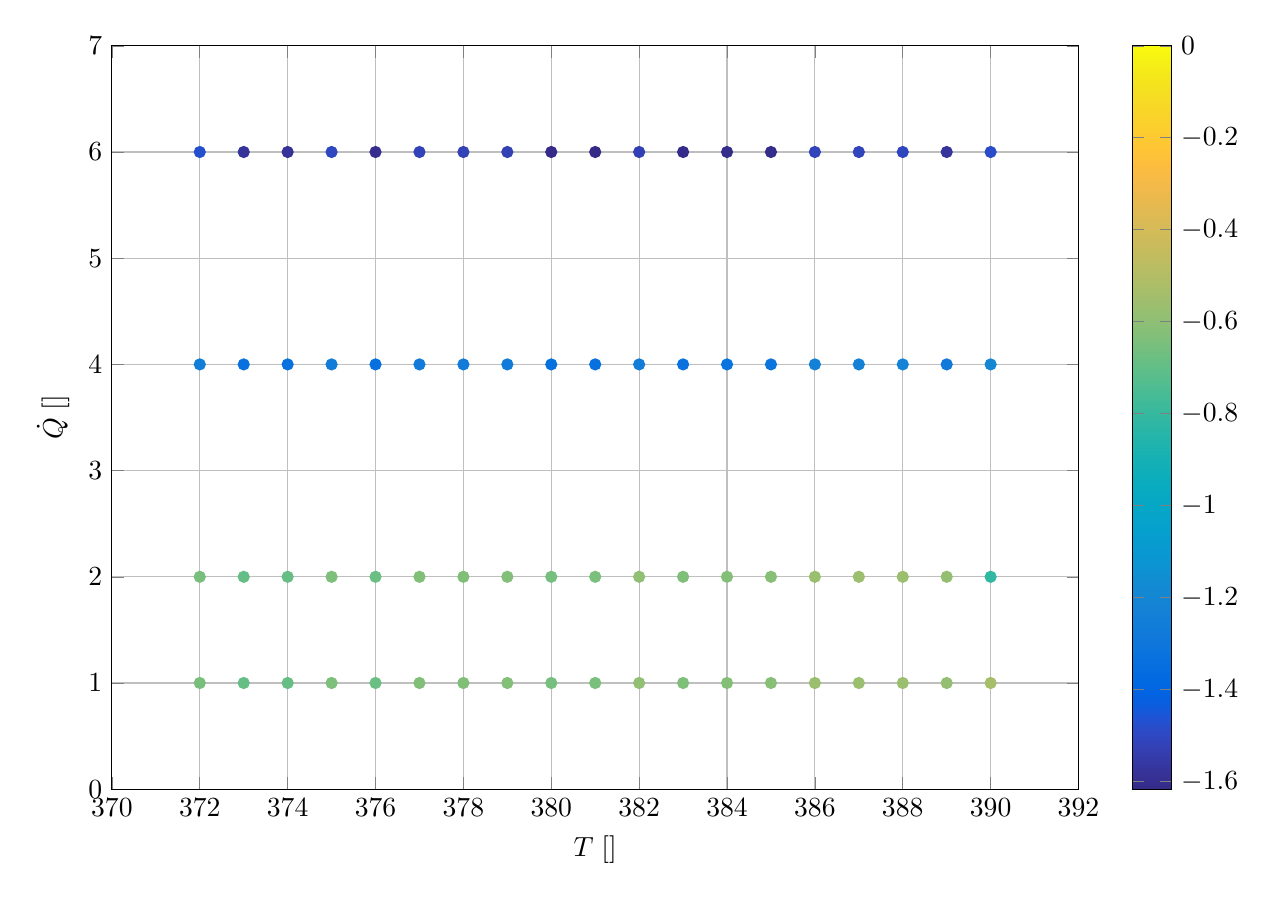
\begin{tikzpicture}

\begin{axis}[%
width=4.833in,
height=3.717in,
at={(0in,0in)},
scale only axis,
point meta min=-1.61662474289174,
point meta max=0,
colormap={mymap}{[1pt] rgb(0pt)=(0.2081,0.1663,0.5292); rgb(1pt)=(0.211624,0.189781,0.577676); rgb(2pt)=(0.212252,0.213771,0.626971); rgb(3pt)=(0.2081,0.2386,0.677086); rgb(4pt)=(0.195905,0.264457,0.7279); rgb(5pt)=(0.170729,0.291938,0.779248); rgb(6pt)=(0.125271,0.324243,0.830271); rgb(7pt)=(0.0591333,0.359833,0.868333); rgb(8pt)=(0.0116952,0.38751,0.881957); rgb(9pt)=(0.00595714,0.408614,0.882843); rgb(10pt)=(0.0165143,0.4266,0.878633); rgb(11pt)=(0.0328524,0.443043,0.871957); rgb(12pt)=(0.0498143,0.458571,0.864057); rgb(13pt)=(0.0629333,0.47369,0.855438); rgb(14pt)=(0.0722667,0.488667,0.8467); rgb(15pt)=(0.0779429,0.503986,0.838371); rgb(16pt)=(0.0793476,0.520024,0.831181); rgb(17pt)=(0.0749429,0.537543,0.826271); rgb(18pt)=(0.0640571,0.556986,0.823957); rgb(19pt)=(0.0487714,0.577224,0.822829); rgb(20pt)=(0.0343429,0.596581,0.819852); rgb(21pt)=(0.0265,0.6137,0.8135); rgb(22pt)=(0.0238905,0.628662,0.803762); rgb(23pt)=(0.0230905,0.641786,0.791267); rgb(24pt)=(0.0227714,0.653486,0.776757); rgb(25pt)=(0.0266619,0.664195,0.760719); rgb(26pt)=(0.0383714,0.674271,0.743552); rgb(27pt)=(0.0589714,0.683757,0.725386); rgb(28pt)=(0.0843,0.692833,0.706167); rgb(29pt)=(0.113295,0.7015,0.685857); rgb(30pt)=(0.145271,0.709757,0.664629); rgb(31pt)=(0.180133,0.717657,0.642433); rgb(32pt)=(0.217829,0.725043,0.619262); rgb(33pt)=(0.258643,0.731714,0.595429); rgb(34pt)=(0.302171,0.737605,0.571186); rgb(35pt)=(0.348167,0.742433,0.547267); rgb(36pt)=(0.395257,0.7459,0.524443); rgb(37pt)=(0.44201,0.748081,0.503314); rgb(38pt)=(0.487124,0.749062,0.483976); rgb(39pt)=(0.530029,0.749114,0.466114); rgb(40pt)=(0.570857,0.748519,0.44939); rgb(41pt)=(0.609852,0.747314,0.433686); rgb(42pt)=(0.6473,0.7456,0.4188); rgb(43pt)=(0.683419,0.743476,0.404433); rgb(44pt)=(0.71841,0.741133,0.390476); rgb(45pt)=(0.752486,0.7384,0.376814); rgb(46pt)=(0.785843,0.735567,0.363271); rgb(47pt)=(0.818505,0.732733,0.34979); rgb(48pt)=(0.850657,0.7299,0.336029); rgb(49pt)=(0.882433,0.727433,0.3217); rgb(50pt)=(0.913933,0.725786,0.306276); rgb(51pt)=(0.944957,0.726114,0.288643); rgb(52pt)=(0.973895,0.731395,0.266648); rgb(53pt)=(0.993771,0.745457,0.240348); rgb(54pt)=(0.999043,0.765314,0.216414); rgb(55pt)=(0.995533,0.786057,0.196652); rgb(56pt)=(0.988,0.8066,0.179367); rgb(57pt)=(0.978857,0.827143,0.163314); rgb(58pt)=(0.9697,0.848138,0.147452); rgb(59pt)=(0.962586,0.870514,0.1309); rgb(60pt)=(0.958871,0.8949,0.113243); rgb(61pt)=(0.959824,0.921833,0.0948381); rgb(62pt)=(0.9661,0.951443,0.0755333); rgb(63pt)=(0.9763,0.9831,0.0538)},
xmin=370,
xmax=392,
xlabel={$T\;[\si{\kelvin}]$},
xmajorgrids,
ymin=0,
ymax=7,
ylabel={$\dot{Q}\;[\si{\kW}]$},
ymajorgrids,
axis background/.style={fill=white},
colorbar
]
\addplot[scatter,only marks,scatter src=explicit,scatter/use mapped color={mark=*,mark options={},draw=mapped color,fill=mapped color}] plot table[row sep=crcr,meta index=2]{%
372	1	-0.651282733331489\\
372	2	-0.651282733331489\\
372	4	-1.24668352086601\\
372	6	-1.47368300371774\\
373	1	-0.691839844081795\\
373	2	-0.691839844081795\\
373	4	-1.33174758141386\\
373	6	-1.57599614247026\\
374	1	-0.68766378682767\\
374	2	-0.68766378682767\\
374	4	-1.33320648059744\\
374	6	-1.58389612940572\\
375	1	-0.63999483746976\\
375	2	-0.63999483746976\\
375	4	-1.26174971472343\\
375	6	-1.50250584807603\\
376	1	-0.678351389377671\\
376	2	-0.678351389377671\\
376	4	-1.34194334299904\\
376	6	-1.60108199193949\\
377	1	-0.630049036879276\\
377	2	-0.630049036879276\\
377	4	-1.26622961250517\\
377	6	-1.51535785522638\\
378	1	-0.6293855686932\\
378	2	-0.6293855686932\\
378	4	-1.26671465422237\\
378	6	-1.51947401938069\\
379	1	-0.62607857702077\\
379	2	-0.62607857702077\\
379	4	-1.26704385895095\\
379	6	-1.52308554709421\\
380	1	-0.654026463821995\\
380	2	-0.654026463821995\\
380	4	-1.34147165280346\\
380	6	-1.61662474289174\\
381	1	-0.646359956582012\\
381	2	-0.646359956582012\\
381	4	-1.33881262395583\\
381	6	-1.61620551976053\\
382	1	-0.59283662508236\\
382	2	-0.59283662508236\\
382	4	-1.25618673295132\\
382	6	-1.52597499593794\\
383	1	-0.631645067425369\\
383	2	-0.631645067425369\\
383	4	-1.32850027151918\\
383	6	-1.61430666054448\\
384	1	-0.62398362821142\\
384	2	-0.62398362821142\\
384	4	-1.32370546613069\\
384	6	-1.61123308383207\\
385	1	-0.61661078842039\\
385	2	-0.61661078842039\\
385	4	-1.31630436585803\\
385	6	-1.60661370936614\\
386	1	-0.567965427159282\\
386	2	-0.567965427159282\\
386	4	-1.23413444148013\\
386	6	-1.51282129998848\\
387	1	-0.567104984403174\\
387	2	-0.567104984403174\\
387	4	-1.23114130659227\\
387	6	-1.51059283137831\\
388	1	-0.564610820212065\\
388	2	-0.564610820212065\\
388	4	-1.22260817738218\\
388	6	-1.50326357144411\\
389	1	-0.583524567021858\\
389	2	-0.583524567021858\\
389	4	-1.28030880314385\\
389	6	-1.57784337046496\\
390	1	-0.536584682787021\\
390	2	-0.812925380625114\\
390	4	-1.19731988028077\\
390	6	-1.48199572485488\\
};
\end{axis}
\end{tikzpicture}%
            }
        \end{figure}
    \end{frame}
    
    
    \subsection*{Conclusions}
    \begin{frame}{Conclusions}
        \begin{itemize}
            \item Test loop is stable under all tested states and phases under the assumptions made.
            \item Pressure and increased heat load are stablizing forces for the system.
        \end{itemize}
    \end{frame}
    
    
    
\section{Future Work}
    \begin{frame}{Future Work}
        \begin{itemize}
            \item \textbf{Modeling:} Explore different, larger, and more complicated geometries with the current toolset.
            \item \textbf{Programming:} Re-write thermodynamics package in a compiled form for increased speed.
            \item \textbf{Numerics:} Improve JFNK solver with built-in fallback routine so full system time-step fallbacks aren't so costly; explore higher-order time stepping algorithms (TR-BDF2).
            \item \textbf{Physics:} Add in more physics to improve on the modeling: boil-off, heat diffusion, true two-phase models.
            \item \textbf{Mathematics:} Examine the non-normal stability matrix using pseudospectra analysis to better assess the effects of short-time transients on the stability of the system.
        \end{itemize}
    \end{frame}
    

    \subsection*{End}
    \begin{frame}[c]{Questions}
        \begin{center}
                ``The key to wisdom is this: constant and frequent questioning. 
                  For by doubting we are led to question, and by questioning we arrive at the truth.''\\
                \hfill --- Peter Abelard
        \end{center}
    \end{frame}







% ======================================================= %
%                       Appendix                          %
% ======================================================= %
\appendix
    
    
    \section{Supplements}
    
    
    % ====================================================================== %
    %                           Stagger/Collocated                           %
    % ====================================================================== %
    \subsection*{Staggered/Collocated}
    \begin{frame}[c,label=Meshes]{Staggered/Collocated}
        \begin{columns}
            \begin{column}[T]{0.4\textwidth}
                Staggered mesh:                
               \begin{center}
                   \includegraphics[height=2.2in]{StaggeredMesh}
               \end{center}
            \end{column}
            \hfill
            \begin{column}[T]{0.4\textwidth}
                Collocated mesh:
                \begin{center}
                    \includegraphics[height=2.2in]{CollocatedMesh}
                \end{center}
            \end{column}
        \end{columns}
    \end{frame}
    
    
    % ====================================================================== %
    %                      Rigorous/Non-rigorous                             %
    % ====================================================================== %
    \subsection*{Rigorous vs. Nonrigorous}
    \begin{frame}[c,label=Nonrigor]{Rigorous vs. Non-Rigorous}\label{Rigorous}
        \begin{columns}
            \begin{column}[T]{0.4\textwidth}
                Rigorous staggered mesh (CFD):                
               \begin{center}
                   \includegraphics[height=2.2in]{StaggeredMesh}
               \end{center}
            \end{column}
            \hfill
            \begin{column}[T]{0.4\textwidth}
                Non-rigorous staggered mesh (System codes):
                \begin{center}
                    \null\vfill
                    \includegraphics[scale=0.325]{NonrigorousMesh}
                    \null\vfill
                \end{center}
                \hfill\textit{\tiny\hyperlink{NonrigorMain}{return}}
            \end{column}
        \end{columns}
    \end{frame}
    
    
    % ====================================================================== %
    %                          Acoustic Speeds                               %
    % ====================================================================== %
    \subsection*{Acoustic Speeds}
    \begin{frame}[c,label=AcousticSpeeds]{Acoustic Speeds}
       \begin{center}
            \includegraphics[height=2.2in]{AcousticSpeedVsMaterialSpeed}
       \end{center}
        \hfill\textit{\tiny\hyperlink{AcousticSpeedsMain}{return}}
    \end{frame}



    % ====================================================================== %
    %                          Non-simple, closed loop                       %
    % ====================================================================== %
    \subsection*{Non-simple, closed loop}
    \begin{frame}[c,label=NonsimpleClosedLoop]{Non-simple, closed loop}
        \begin{center}
            \includegraphics[height=2.2in]{ComputationalGeometry}
        \end{center}
    \end{frame}
    
    
    % ====================================================================== %
    %                          Non-simple, closed loop                       %
    % ====================================================================== %
    \subsection*{i-rho Space}
    \begin{frame}[c,label=irhoSpace]{$i$-\rho Diagram}
        \begin{center}
            \includegraphics[height=2.2in]{InteEnergyVsDensity}
        \end{center}
        \hfill\textit{\tiny\hyperlink{EOS}{return}}
    \end{frame}
    
    
    
    % ====================================================================== %
    %                            Stability Diagrams                          %
    % ====================================================================== %
    \subsection*{Stability Diagrams}
    \begin{frame}[c,label=StabilityDiagrams]{Stability Diagrams}
        \begin{columns}
            \begin{column}[T]{0.4\textwidth}
                Linearly stable, nonlinearly unstable:
                \begin{center}
                    \vspace{0.09in}
                    \includegraphics[height=0.91in]{LinearlyStableNonlinearlyUnstable}
                \end{center}
            \end{column}
            \hfill
            \begin{column}[T]{0.4\textwidth}
                Linearly unstable, nonlinearly stable:
                \begin{center}
                    \null\vfill
                    \includegraphics[height=0.83in]{LinearlyUnstableNonlinearlyStable}
                    \null\vfill
                \end{center}
                \hfill\textit{\tiny\hyperlink{Perturbation}{return}}
            \end{column}
        \end{columns}
    \end{frame} 
    
    
    
    % ====================================================================== %
    %                            Stability Diagrams                          %
    % ====================================================================== %
    \subsection*{System Mass flow: 4 days}
    \begin{frame}[c,label=MassFlow4Days]{System Mass flow: 4 days}
        \begin{center}
            \includegraphics[height=2.4in]{MassRateFor4days}
        \end{center}
        \hfill\textit{\tiny\hyperlink{MassFlowAnnotate}{return}}
    \end{frame}
    
    
    
    % ====================================================================== %
    %                             Multiphase Model                           %
    % ====================================================================== %
    \subsection*{Multiphase Model}
    \begin{frame}[label=Multiphase]{Multiphase Model}
         \begin{equation}
            \renewcommand{\arraystretch}{2.2}
            \pdiff{}{t}\begin{bmatrix}
                           \rhok \\
                           \rhouk \\
                           \rhoik 
                        \end{bmatrix}
            + 
            \pdiff{}{z}\begin{bmatrix}
                            \rhouk                 \\
                            \uk\,    \rhouk  + P(\rho\subs{\phi},\ik)   \\
                            \uk\left[\rhoik  + P(\rho\subs{\phi},\ik)\right]
                        \end{bmatrix}
                     = 
        \end{equation}
        \begin{equation}\renewcommand{\arraystretch}{2.2}
            \begin{bmatrix}
                \mathbb{M}\subs{\phi} \\
                \rhok{g(z)} - \frac{\Keff\subs{,\phi}(\qCon)}{2} \uk\,|\rhouk| + \mathbb{P}\subs{\phi}  \\
                \dot{Q}\subs{add,\phi}(\qCon,z,t) + \mathbb{E}\subs{\phi}
            \end{bmatrix}
            \notag
        \end{equation}
    \end{frame}


\end{document}

